%% This template is based on the work of Ruben De Smet (https://gitlab.com/rubdos/texlive-vub) and altered further to create a more general template for the Master thesis's report submission within the BruFacE-programme.
%% Further alterations implemented by Nick Van Goethem
%% License: LaTeX Project Public License 1.3c

%% According to the BruFacE's Master thesis regulations, the students must hand in a double-sided hard copy version of the Master thesis to each member of the jury + ONE for the secretariat, while also forwarding an electronic version to the faculty Secretariat
%% To save the according PDF's you must type in the following document-classes for the:
%	- electronic version
\documentclass[11pt,notitlepage]{report}
%	- double-sided (to print) version
% \documentclass[11pt,twoside,notitlepage]{report}
%% and save/download each run seperately
\usepackage{brufaceStyle}
%% you can add other languages by changing or adding them to the babel-package between []
%\usepackage[T1]{fontenc}
\usepackage[english,french,dutch]{babel}
\usepackage{helvet} % helvetica font for front page and abstract heading
\usepackage{amsmath,amssymb} % provides the symbols for mathematical expressions
\usepackage{siunitx} % provides the SI units
\usepackage{titlesec} % to adjust the spacing before and after the chapter
\usepackage{graphicx}
\usepackage{wrapfig}
\usepackage{epsfig}
\usepackage{tabularx}
\usepackage{multirow}
\usepackage{tablefootnote}
\usepackage{subcaption}
\usepackage{setspace}
\usepackage{sectsty}
\usepackage[titles]{tocloft}
\setlength{\cftbeforechapskip}{5pt} % reduces the spacing between chapters in the table of content
\usepackage{lipsum}
\usepackage[hidelinks]{hyperref}
\usepackage{cleveref}
\usepackage[acronyms,toc,nonumberlist,nogroupskip,automake,nopostdot]{glossaries}
\usepackage{listings}
\usepackage{fancyhdr}
\usepackage{tikz}
\sisetup{detect-all}

\pagestyle{fancy}
\fancyhf{}
\setlength{\headheight}{14pt}
\fancyhead[RE]{\rightmark}
\fancyhead[LO]{\leftmark}
\fancyhead[LE,RO]{\thepage}
\fancyfoot[RO]{\begin{picture}(0,0) \put(20,755){\vubtriangle} \end{picture}}
\fancyfoot[LE]{\begin{picture}(0,0) \put(-33,766){\ulbtriangle} \end{picture}}

\makeatletter
%%% redefine \eqref to be like the original
\renewcommand{\eqref}[1]{\textup{\eqreftagform@{\ref{#1}}}}
\let\eqreftagform@\tagform@
%%% redefine \tagform@
\def\tagform@#1{%
	\maketag@@@{%
		\if@unit\ensuremath{\left[\thiseq@unit\right]}\quad\fi\global\@unitfalse
		(\ignorespaces#1\unskip\@@italiccorr)%
	}%
}
\newif\if@unit
\def\equnit#1{%
	\gdef\thiseq@unit{#1}%
	\global\@unittrue
}
\makeatother

%% adjusts the spacing above and below the chapter title
\titleformat{\chapter}[display]{\normalfont\LARGE\bfseries}{\chaptertitlename\ \thechapter}{0pt}{\Huge}
\titlespacing*{\chapter}{0pt}{0pt}{10pt}

%% redefines the title of \right) he table of contents
\addto\captionsenglish{% Replace "english" with the language you use
	\renewcommand{\contentsname}%
	{Table of Contents}%
}
%% ---------------------------------------Title Page---------------------------------------
\title{A frequency domain approach to data-driven control}
% \subtitle{Here goes a possible subtitle of the thesis (this extra text is added to see how the title-page would look like with a very long inserted subtitle)}
\author{Marc Berneman}
%% general information about your promotor(s) and academic year (TO BE COMPLETED)
\academicYear{2019 -- 2020}
\promotor{Prof.\ Dr.\ Ir.\ Rik Pintelon}
\coSupervisor{Prof.\ Dr.\ Ir.\ John Lataire}
%% uncomment the Master program (and its major) to display in the document
%\masterAndMajor{Master of Science in Architectural Engineering}{}
%\masterAndMajor{Master of Science in Chemical and Materials Engineering}{major in Materials}
%\masterAndMajor{Master of Science in Chemical and Materials Engineering}{major in Process Technology}
%\masterAndMajor{Master of Science in Civil Engineering}{}
%\masterAndMajor{Master of Science in Electromechanical Engineering}{major in Aeronautics}
%\masterAndMajor{Master of Science in Electromechanical Engineering}{major in Energy}
%\masterAndMajor{Master of Science in Electromechanical Engineering}{major in Mechatronics-Construction}
% \masterAndMajor{Master of Science in Electromechanical Engineering}{major in Vehicle Technology and Transport}
\masterAndMajor{Master of Science in Electrical Engineering}{major in Measuring, Modeling and Control}

%% There are two different defined geometries, one for the electronic version, and one for the double-sided print-version (CHOOSE that one you would like to save)
%	- electronic version
\geometry{top=2.5cm,bottom=2.25cm,left=3cm,right=3cm}
%	- double-sided print version
%\geometry{top=2.5cm,bottom=2.5cm,inner=3.5cm,outer=2.5cm}

%\allsectionsfont{\normalfont\sffamily\bfseries} % applies sans serif font to the headings
%% ----------------- here we make the list of symbols and abbreviations --------------------
\newglossary[slg]{symbols}{sym}{sbl}{List of Symbols} % create add. symbolslist
%% here we define the symbol listing environment, DO NOT ALTER !!!
\glsaddkey{unit}{\glsentrytext{\glslabel}}{\glsentryunit}{\GLsentryunit}{\glsunit}{\Glsunit}{\GLSunit}\glssetnoexpandfield{unit}
\setlength{\glsdescwidth}{15cm} % sets the width of the glossary environment
\newglossarystyle{symbunitlong}{%
	\setglossarystyle{super3col}% base this style on the list style
	\renewenvironment{theglossary}{% Change the table type --> 3 columns
		\begin{supertabular}{p{8mm}p{0.8\glsdescwidth}>{\centering\arraybackslash}p{2cm}}}%
		{\end{supertabular}}%
	%
%	\renewcommand*{\glossaryheader}{%  Change the table header
%		\bfseries Symbol & \bfseries Description & \bfseries Unit \\
%		\endhead}
	\renewcommand*{\glossentry}[2]{%  Change the displayed items
		\glstarget{##1}{\glossentryname{##1}} %
		& \glossentrydesc{##1}% Description
		& \glsunit{##1}  \tabularnewline
	}
}
%%-------Here starts the file in which the actual acronyms and symbols are putted in--------
%--------------------------------------------------------------------------
%% Below, we define all the acronyms we want to use throughout the document
%--------------------------------------------------------------------------
\newacronym{lti}{LTI}{Linear time-invariant}
\newacronym{ct}{CT}{Continuous-time}
\newacronym{dt}{DT}{Discrete-time}
\newacronym{td}{TD}{Time domain}
\newacronym{fd}{FD}{Frequency domain}
\newacronym{dft}{DFT}{Discrete Fourier transform}
\newacronym{idft}{IDFT}{Inverse discrete Fourier transform}
\newacronym{frf}{FRF}{Frequency response function}
\newacronym{zoh}{ZOH}{Zero-order hold}
\newacronym{lpm}{LPM}{Local Polynomial Method}
\newacronym{rms}{RMS}{Root mean square}
\newacronym{mse}{MSE}{Mean squared error}
\newacronym{snr}{SNR}{Signal-to-noise ratio}
\newacronym{nsr}{NSR}{Noise-to-signal ratio}
\newacronym{wnls}{WNLS}{Weighted nonlinear least squares}
\newacronym{hf}{HF}{High-frequency}
\newacronym{dc}{DC}{Direct current}
\newacronym{cl}{CL}{Closed loop}
\newacronym{bla}{BLA}{Best linear approximation}
\newacronym{opamp}{OPAMP}{Operational amplifier}

%--------------------------------------------------------------------------
%% Below, we define all the symbols we want to use throughout the document
%--------------------------------------------------------------------------
\newglossaryentry{symb:G(s)}{name=\ensuremath{G(s)},
	description={Continuous-time transfer function},
	unit={-},
	type=symbols}
	
\newglossaryentry{symb:G(z^-1)}{name=\ensuremath{G(z^{-1})},
	description={Discrete-time transfer function},
	unit={-},
	type=symbols}

\newglossaryentry{symb:u}{name=\ensuremath{u},
	description={Input in the time domain},
	unit={-},
	type=symbols}
	
\newglossaryentry{symb:U}{name=\ensuremath{U},
	description={Input in the frequency domain},
	unit={-},
	type=symbols}
	
\newglossaryentry{symb:y}{name=\ensuremath{y},
	description={Output in the time domain},
	unit={-},
	type=symbols}
	
\newglossaryentry{symb:Y}{name=\ensuremath{Y},
	description={Output in the frequency domain},
	unit={-},
	type=symbols}
	
\newglossaryentry{symb:r}{name=\ensuremath{r},
	description={Reference in the time domain},
	unit={-},
	type=symbols}
	
\newglossaryentry{symb:R}{name=\ensuremath{R},
	description={Reference in the frequency domain},
	unit={-},
	type=symbols}
	
\newglossaryentry{symb:fs}{name=\ensuremath{f_s},
	description={Sampling frequency},
	unit={Hz},
	type=symbols}
	
\newglossaryentry{symb:ts}{name=\ensuremath{T_s},
	description={Sampling period},
	unit={s},
	type=symbols}
	
\newglossaryentry{symb:N}{name=\ensuremath{N},
	description={number of samples used in the DFT},
	unit={-},
	type=symbols}
\makeglossaries
%% -------------------Here starts all the basic code for the document-----------------------


\usepackage{amsmath}
\usepackage{xcolor}
\usepackage{todonotes}
\usepackage{amssymb}
\usepackage{hyperref}
\usepackage{dsfont}
\usepackage{float}
\usepackage{appendix}
\usepackage{chngcntr}
\newcommand{\kexc}{\text{K}_{\text{exc}}}
%\usepackage{multibib}
%\newcites{soft}{Software}

\AtBeginEnvironment{subappendices}{%
\chapter*{Appendix}
\addcontentsline{toc}{chapter}{Appendices}
\counterwithin{figure}{section}
\counterwithin{table}{section}
}

\begin{document}
\maketitle
\pagestyle{empty}
\textcolor{white}{This is done in order to skip the first half of the page}\\
\fontsize{10}{12}

%\vspace{13cm}
\vspace{21cm}% when you would not have a confidentiality claus

%% if you have a confidentiaity claus with the university or a third party, uncomment the text below and fill in the proper embargo date
%\noindent\textsf{Confidential up to and including dd/mm/20xx}\\
%\noindent\textsf{Important}\\
%
%\vspace{5mm}
%
%\noindent\textsf{This master dissertation contains confidential information and/or confidential research results proprietary to the \textit{Vrije Universiteit Brussel}, \textit{Universit\'{e} Libre de Bruxelles} or third parties. It is strictly forbidden to publish, cite or make public in any way this master’s dissertation or any part thereof without the written permission of the author(s), the \textit{Vrije Universiteit Brussel}, the \textit{Universit\'{e} Libre de Bruxelles} and/or the third parties involved.}\\ 
%
%\noindent\textsf{Under no circumstance may this master dissertation be communicated to or put at the disposal of other third parties. Photocopying or duplicating it in any other way is strictly prohibited.
%Disregarding the confidential nature of this master dissertation may cause irremediable damage to the \textit{Vrije Universiteit Brussel}, \textit{Universit\'{e} Libre de Bruxelles} or third parties involved.}\\
%\noindent\textsf{The stipulations mentioned above are in force until the embargo date.}\\
%
%\vspace{5mm}

\noindent\textsf{The author(s) gives (give) permission to make this master dissertation available for consultation and to copy parts of this master dissertation for personal use. In all cases of other use, the copyright terms have to be respected, in particular with regard to the obligation to state explicitly the source when quoting results from this master dissertation.}\\

%if no particular confidentianlity has been used, just use the date of the thesis' deadline
\noindent\textsf{17/08/2020}
\clearpage
%% front matter
\pagenumbering{Roman} % Roman page numbering for the front matter
\pagestyle{plain}
%% here, the files for the abstract are added for the english version (first language) and possible extra native languages (second and third) -- you can comment which ever one is obsolete

\chapter*{Acknowledgements}
\addcontentsline{toc}{chapter}{Acknowledgements}
Over the past 5 years I have been given a very broad education in Electrical Engineering and Engineering in general. Of all the courses I took, the ones about System and Control theory have fascinated me the most. I am therefore very grateful to have been given the opportunity to write my Master thesis about this topic.\\

\noindent
I would like to thank my supervisor Professor Pintelon and co-supervisor Professor Lataire for all their guidance and patience. They have given me the freedom to pursue my research interests, but they guided me when I needed it. \\

\noindent
I also want to express my gratitude to all the professors, assistants and lab personnel at the VUB and ULB who have shaped me into the engineer I am today.\\

\noindent
Finally, I wish to thank my parents for their support and encouragement throughout my study.\\


\noindent
August 2020,

\noindent
Marc Berneman

\addcontentsline{toc}{chapter}{Abstract}
\selectlanguage{english}
\masterTitle{Title}{A frequency domain approach to data-driven control}
\authorThesis{Author}%in this input frame you write "Author" in the language of the abstract
\Master{Master of Science in Electrical Engineering -- major in Measuring, Modeling and Control}% here you have to write the full title of your Master programme
\yearTitle{Academic year}
%% in this environment, you will write your abstract. Keep it limited to a SINGLE PAGE. Max. 500 words should normally do the trick
\begin{abstract}
	\section*{Abstract}\label{sec:abstract}
% 	\addcontentsline{toc}{section}{\nameref{sec:abstract}}
	%% start adjusting the abstract from here on
	{\fontsize{10}{16}
	%\setstretch{1.05}
    
Data-driven model reference control allows for the design of a controller from input and output data when a parametric model of the system is not available. It is already known how to do this for discrete-time systems. 
%By using nonparametric models of the frequency response function of linear time-invariant systems it is possible to generalize model reference control to continuous-time systems. 
In this thesis we propose to generalize model reference control to continuous-time systems.
Moreover, it is demonstrated how the stability of the closed loop system can be guaranteed by using the small-gain theorem. The proposed methods are used to design an analog controller for a continuous-time system.

	\vspace{5mm}
	\noindent\textbf{Keywords:} data-driven controller tuning; model reference control; frequency domain approach; nonparametric; frequency response function
	}
    
\end{abstract}
\newpage
\restoregeometry
%% here comes the preface, if desired -- here you can add personal comments and make acknowledgements (comment if you do not need this inside the thesis)
% \setstretch{1.1}
% \input{text/preface.tex}
%%-----------------------------------table of contents--------------------------------------------
\selectlanguage{english}
{\fontsize{12}{16}
	\tableofcontents
	\addcontentsline{toc}{chapter}{Table of Contents}
	%% you can change the structure of letting the lists together on the same page or start a new page each time, that is up to you
% 	\clearpage
% 	{
% 	\let\clearpage\relax
% 	\listoffigures\addcontentsline{toc}{chapter}{List of Figures}
% 	\listoftables\addcontentsline{toc}{chapter}{List of Tables}
% 	}%
	{
		\glsaddall % adds all the acronyms and symbols to their respective lists
		\printglossary[type=\acronymtype,title={List of Abbreviations},style=long]
		% list of acronyms
% 		\let\clearpage\relax
% 		\printglossary[type=symbols,style=symbunitlong]   % list of symbols
	}
}%
%%--------------------------------------main matter-----------------------------------------------
\newpage
\addcontentsline{toc}{part}{A frequency domain approach to data-driven control}

\pagenumbering{arabic}
\pagestyle{fancy}

\chapter{Introduction}


Systems that react to stimuli are all around us. However, many systems don't behave as we want them to. Control theory is a framework that allows engineers to find ways to manipulate these stimuli in order to get these systems to behave as they want them to. Traditionally, the first step to controlling a system is to model the underlying system. If the system is a linear time-invariant (LTI) system, it can be modelled by a transfer function or state space equations. This transfer function or state space model is a parametric representation of the system. When a parametric model of the system is obtained, a controller can be designed for it. 

A model of an LTI system can be obtained by applying a well-designed input to the system and measuring the corresponding output.

Data-driven control is an attempt to skip the modelling part of this process. Instead of going from data to a parametric model to a controller, a controller is found directly from data. This is illustrated in figure \ref{fig:data-driven_vs_tradition}.

One such data-driven approach is model reference control \cite{Data-driven_model_reference_control}. The idea is to define a reference model and to tune a controller such that the closed loop system is as close as possible to the reference model. However, as will be shown in chapter \ref{chapter:model_reference_control}, the name ``data-driven'' can be a bit misleading. In fact, it will be shown that a nonparametric model is hidden in the maths. A nonparametric model differs from a parametric model in the sense that the parametric model tries to describe the data using a relatively small amount of parameters. A nonparametric model still has parameters, but the amount of parameters can be equal to the number of data points. Concretely, applied to LTI systems, a parametric model could be a transfer function where the parameters are the coefficients of the numerator and denominator. A nonparametric model of an LTI system could be the frequency response function at different frequencies.

Chapter \ref{chapter:preliminaries} gives an introduction to nonparametric models of LTI systems. Chapter \ref{chapter:model_reference_control} explains model reference control and shows that there is an underlying nonparametric model in the maths. Chapter \ref{chapter:guaranteed_stability} shows how stability can be guaranteed in model reference control in the absence of a parametric model and in chapter \ref{chapter:real_experiment} model reference control is used to design a controller for a real system.


\begin{figure}
\centering
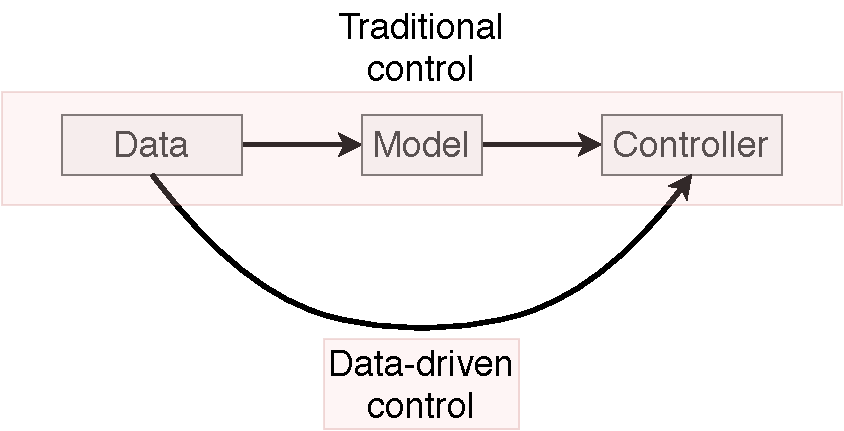
\includegraphics[width = 0.7\textwidth]{figures/data-driven_vs_tradition.pdf}
\caption{Traditional control vs. data-driven control.}
\label{fig:data-driven_vs_tradition}
\end{figure}



\counterwithout{figure}{subsection}
\counterwithout{table}{subsection}
\counterwithout{figure}{section}
\counterwithout{table}{section}
\counterwithin{figure}{chapter}
\counterwithin{table}{chapter}
\chapter{Preliminaries}
\label{chapter:preliminaries}
\section{Introduction}
A refresher about linear time-invariant systems is given here. Afterwards, this section focuses on frequency domain (FD) methods for estimating nonparametrically the frequency response function (FRF). White noise and system transients are analysed in the FD. It is important to understand how white noise manifests itself in the frequency domain as it will increase the variability of the nonparametric estimate of the FRF. System transients not only increase the variability of the FRF estimates but also introduce a bias error. Therefore, it is also important to study its properties so that it can be accounted for during nonparametric estimation of the FRF. Finally, this chapter ends with some advanced methods to suppress transients and noise in FRF estimation.


\section{LTI systems}
Linear time-invariant (LTI) systems can be represented in different ways. In this work, we will use the transfer function (TF) representation for single-input single-output (SISO) systems.
\begin{equation*}
    G(\Omega) = \frac{B(\Omega)}{A(\Omega)}
\end{equation*}
with
\begin{equation*}
    \Omega = \begin{cases}
        s & \text{if working in continuous-time (CT)} \\
        z^{-1} & \text{if working in discrete-time (DT)} 
    \end{cases}
\end{equation*}
and $B(\Omega)$ and $A(\Omega)$ being polynomials of $\Omega$. 
%The order of $B(\Omega)$ should not exceed the order of $A(\Omega)$ in order to preserve causality.
For now, we will keep our focus on CT systems. In CT, the output of this system is given by
\begin{equation*}
    y(t) = \mathcal{F}^{-1}\{Y(j\omega)\} = \mathcal{F}^{-1}\{G(j\omega) U(j\omega)\} = \mathcal{F}^{-1}\{G(j\omega) \mathcal{F}\{u(t)\}\}
\end{equation*}
With $\mathcal{F}$ and $\mathcal{F}^{-1}$ denoting the Fourier transform and inverse Fourier transform respectively.
\begin{align*}
    \mathcal{F}\{x(t)\}\}(j\omega) &= \int_{-\infty}^{+\infty} x(t) e^{-j \omega t} dt \\
    \mathcal{F}^{-1}\{X(j\omega)\}(t) &= \frac{1}{2\pi} \int_{-\infty}^{+\infty} X(j\omega) e^{j \omega t} d \omega 
\end{align*}
Because a convolution in the time domain (TD) becomes a multiplication in the frequency domain, the output in the FD is simply found by performing a multiplication.
\begin{equation}
\boxed{
    Y(j\omega) =G(j\omega) U(j\omega)
    }
    \label{eq:Y=GU}
\end{equation}

\newpage
\section{Single sine excitations}
Assume that the input $u(t)$ of the system is a complex exponential with a single frequency.
\begin{equation*}
    u(t) = e^{j (\omega_u t + \phi)}
\end{equation*}
In the FD this becomes
\begin{equation*}
    U(j\omega) = 2\pi e^{j\phi} \delta(\omega-\omega_u)
\end{equation*}
With $\delta$ denoting the Dirac delta function. Using (\ref{eq:Y=GU}) gives the output in the FD is
\begin{equation*}
    Y(j\omega) = 2\pi |G(j\omega_u)| e^{j(\phi+\angle{G(j\omega_u)})} \delta(\omega-\omega_u)
\end{equation*}
Transforming back to the TD we find
\begin{equation*}
    y(t) = |G(j\omega_u)| e^{j \angle{G(j\omega_u)}} e^{j (\omega_u t + \phi)} = |G(j\omega_u)| e^{j \angle{G(j\omega_u)}} u(t)
\end{equation*}
Since the system is linear and real, this result can be used to calculate the output of the system if the input is a cosine wave.
\begin{equation*}
    u(t) = \cos{(\omega_u t + \phi)} = \frac{e^{j(\omega_u t + \phi)}+e^{-j(\omega_u t + \phi)}}{2}
\end{equation*}
After a brief calculation, the output is found to be given by
\begin{equation*}
\boxed{
    y(t) = |G(j\omega_u)| \cos{(\omega_u t + \angle{G(j\omega_u)} + \phi)}
    }
\end{equation*}

To summarize, if the input of a system is a sine wave, then the output will be a sine wave with the same frequency, but with a different phase and amplitude determined by the value of the transfer function at that frequency.

\section{Discrete Fourier transform}
Using the Fourier transform is not practical as it requires an infinite amount of data and an infinite time resolution to compute. The discrete Fourier transform (DFT) solves both of these problems.

The DFT of a sequence $x(n)$, $n = 0,1,\ldots,N-1$ is defined as
\begin{equation*}
    X(k) = \text{DFT}\{x(n)\} = \frac{1}{N}\sum_{n=0}^{N-1} x(n) e^{-j 2\pi k n/N} \,,\quad k \in \mathds{Z}
\end{equation*}
$X(k)$ is periodic with period $N$, so $k$ is usually confined to $k = 0,1 \ldots, N-1$. Usually, the DFT is defined without the factor $\frac{1}{N}$. However, this will simplify the notation in this work. The inverse DFT (IDFT) is defined in a similar way.
\begin{equation*}
    x(n) = \text{IDFT}\{X(k)\} = \sum_{k=0}^{N-1} X(k) e^{j 2\pi k n/N} \,,\quad n \in \mathds{Z}
\end{equation*}

\newpage
\section{Perfect reconstruction}
The question now is: under which conditions can we perfectly reconstruct a CT signal $x(t)$ from a DT measurement?
\begin{equation*}
    x_d(n) = x(n T_s) \,,\quad n = 0,\ldots,N-1
\end{equation*}
It is simpler to see when this is the case by working in the FD. The question then becomes: under which conditions does the DFT of $x_d(n)$ contain the same information as the Fourier transform of $x(t)$?

\paragraph{Periodicity}
First, as the DFT has a limited spectral resolution, the Fourier spectrum of the continuous signal must also be discrete. This is the case when the CT signal is periodic. If the CT signal has a period $T$
\begin{equation*}
    x(t) = x(t+T) \quad \forall t
\end{equation*}
then the Fourier spectrum of $x(t)$ will consist of Dirac delta functions with a fixed spacing between the Dirac pulses.
\begin{equation*}
    X(\omega) = \mathcal{F}\{x(t)\} = \sum_{n=-\infty}^{+\infty} c_n \delta(\omega - n \omega_0) \,,\quad \omega_0 = \frac{2\pi}{T}
\end{equation*}

\paragraph{Leakage}
Next, the DFT frequencies should coincide with the Dirac pulses to avoid leakage. The DFT bins $k$ correspond to certain frequencies depending on the sampling frequency $f_s$ and the number of samples $N$.
\begin{equation*}
    \omega_k = 2 \pi k \frac{f_s}{N} = 2 \pi k \frac{1}{N T_s} = 2 \pi k \frac{1}{T_{\mathrm{meas}}}
\end{equation*}
$T_{\mathrm{meas}} = N T_s$ is the measurement time. The lowest frequency of the CT signal $\omega_{\mathrm{signal}}$ needs to correspond to one of the DFT frequencies in order to avoid leakage.
\begin{equation*}
    \omega_{\mathrm{signal}} = \omega_k \Rightarrow \boxed{T_{\mathrm{meas}} = k T_{\mathrm{signal}}}
\end{equation*}
In simple words: the measurement time must contain an integer number of periods of the CT signal.

\paragraph{Aliasing}
Finally, the famous Nyquist-Shannon sampling theorem states that the CT signal $x(t)$ must not contain frequency components higher than half the sampling frequency.
\begin{equation*}
    f_{\mathrm{max}} < \frac{f_s}{2}
\end{equation*}

To summarize, a CT signal is perfectly reconstructable from a sampled version of it in a limited time window if the DFT contains the same information as the CT Fourier transform. This is the case when the following conditions are met:

\begin{itemize}
    \item The CT signal is periodic.
    \item The measurement time contains an integer number of periods.
    \item The bandwidth of the signal does not exceed half the sampling frequency.
\end{itemize}

\newpage
\section{Frequency response function estimation}
If the input and output of an LTI system satisfy the conditions of perfect reconstructability, then the transfer function can be calculated at the excited frequencies. Taking the input to be a periodic single sine as before results in a sine in the output with the same frequency.
\begin{equation*}
    u(t) = \cos{(\omega_u t + \phi)} \Rightarrow y(t) = |G(j\omega_u)| \cos{(\omega_u t + \angle{G(j\omega_u)} + \phi)}
\end{equation*}
In the FD this becomes
\begin{equation*}
    Y(j\omega_u) = G(j\omega_u) U(j\omega_u)
\end{equation*}
Assuming that the excited frequency corresponds to one of the DFT frequencies $\omega_u = \omega_k = 2 \pi k f_s/N$  and $|\omega_k| < \pi f_s$ fulfils the last 2 conditions of perfect reconstructability respectively.
% \begin{equation*}
%     U(k) = N U(j \omega_k) \,,\quad Y(k) = N Y(j \omega_k) \,,\quad \omega_k = 2 \pi k f_s/N \,,\quad  0 \leq k < N
% \end{equation*}
\begin{equation*}
     U(j\omega_k) = 2\pi U(k)  \delta(\omega-\omega_k) \,,\quad Y(j\omega_k) = 2\pi Y(k)  \delta(\omega-\omega_k)
\end{equation*}
With $U(k)$ and $Y(k)$ being the $k$-th DFT bin of $u_d(n)$ and $y_d(n)$ respectively. Note that the factor $2\pi$ is just a consequence of how the Fourier transform and the DFT are defined. In the end, we are interested in ratios, so this won't matter. This means that
\begin{equation}
    Y(k) = G(j\omega_k) U(k)
    \label{eq:Y=GU_DFT}
\end{equation}
Finally, the value of the frequency response function at $s = j\omega_k$ can be calculated as
\begin{equation*}
    \boxed{
    G(j\omega_k) = \frac{Y(k)}{U(k)}
    }
\end{equation*}

\section{Multisine excitations}
Using a single sine excitations allows to calculate the value of the FRF at one single frequency. We can make use of the linearity of LTI systems to calculate the FRF at multiple frequencies at once. This is where a multisine excitation can be useful.
\begin{equation*}
    u(t) =  \sum_{k \in \kexc} A_k \sin(\omega_k t + \phi_k) \,,\quad \omega_k = 2 \pi k \frac{f_s}{N} \,,\quad \kexc \subseteq \{n \in \mathds{Z} | 0 \leq n < N/2 \}
\end{equation*}
In the FD this gives
\begin{equation*}
    U(k) = \frac{A_k}{2j} e^{j \phi_k} \,,\quad k \in \kexc
\end{equation*}
By using (\ref{eq:Y=GU_DFT}) the output is
\begin{equation*}
    Y(k) = G(j \omega_k) \frac{A_k}{2j} e^{j \phi_k} \,,\quad k \in \kexc
\end{equation*}
Thus, the FRF can be calculated for all $k \in \kexc$.
\begin{equation}
    G(j\omega_k) = \frac{Y(k)}{U(k)} \,,\quad k \in \kexc
    \label{eq:G=Y/U_MS}
\end{equation}

\paragraph{Magnitude choice}
The magnitude of the sine components $A_k$ can be chosen by the user. This can be useful when noise occurs in a certain frequency band. More power can be attributed to this frequency band to get a better signal-to-noise ratio at those frequencies.

\paragraph{Phase choice}
The phases of the sine components $\phi_k$ can also be chosen by the user. A concise example is given to see what the consequences are of choosing a different phase. Two possibilities are shown here.

A linear phase multisine is the simplest case: all the sine components have the same phase 
\begin{equation*}
    \phi_k=0
\end{equation*}

In a random phase multisine the phases of the sine components have random phases drawn from a uniform distribution between $0$ and $2 \pi$.
\begin{equation*}
    \phi_k \sim \mathcal{U}(0,2\pi)
\end{equation*}

Two multisines with the same RMS values are shown in figure \ref{fig:linear_random_MS_compare}. One has a linear phase, while the other has a random phase. The magnitude spectrum of both are the same. However, the linear phase multisine peaks at $t=0$, while the power of the random phase multisine is more evenly distributed over time. This can be useful when the generator has a limited range due to saturation. Even though both signals contain the same power, the random phase multisine is less likely to saturate.

\begin{figure}[H]
    \centering
    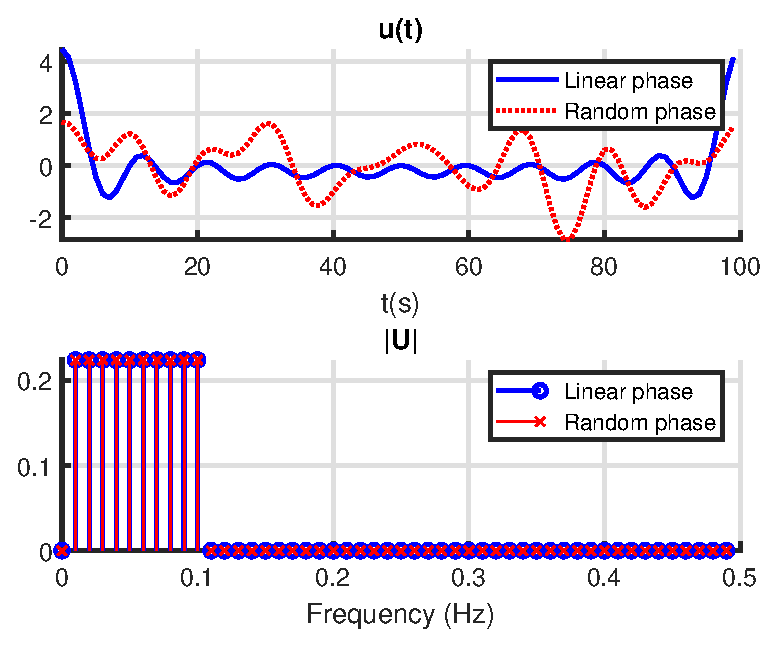
\includegraphics[width = 0.65\textwidth]{figures/MS_u0_u.eps}
    \caption{Comparison between a linear phase multisine and a random phase multisine with the same RMS value.}
    \label{fig:linear_random_MS_compare}
\end{figure}

\newpage
\paragraph{Example}
Consider a DT system.
\begin{equation}
    G(z^{-1}) = \frac{0.4097 z^{-1} + 0.407 z^{-2}}{1 - 1.165 z^{-1} + 0.9813 z^{-2}}
    \label{eq:Gz_example}
\end{equation}
This system is excited by the random phase multisine shown in figure \ref{fig:MS_u}. The normalized frequency is the frequency divided by the sampling frequency. 0.5 represents the Nyquist frequency $f_s/2$. The steady state output of this system is shown in figure \ref{fig:MS_y}. Then the FRF can be calculated by using (\ref{eq:G=Y/U_MS}) at the excited frequencies. The actual FRF and calculated FRF are plotted in figure \ref{fig:MS_G}.

\begin{figure}[H]
    \centering
    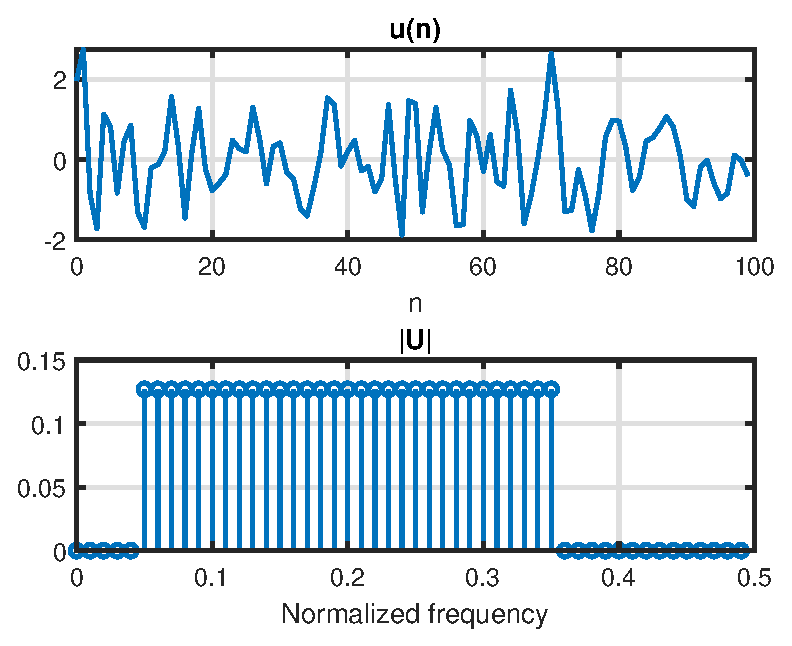
\includegraphics[width=0.65\textwidth]{figures/MS_u.eps}
    \caption{Input of the second-order system. Random phase multisine.}
    \label{fig:MS_u}
\end{figure}

\begin{figure}[H]
    \centering
    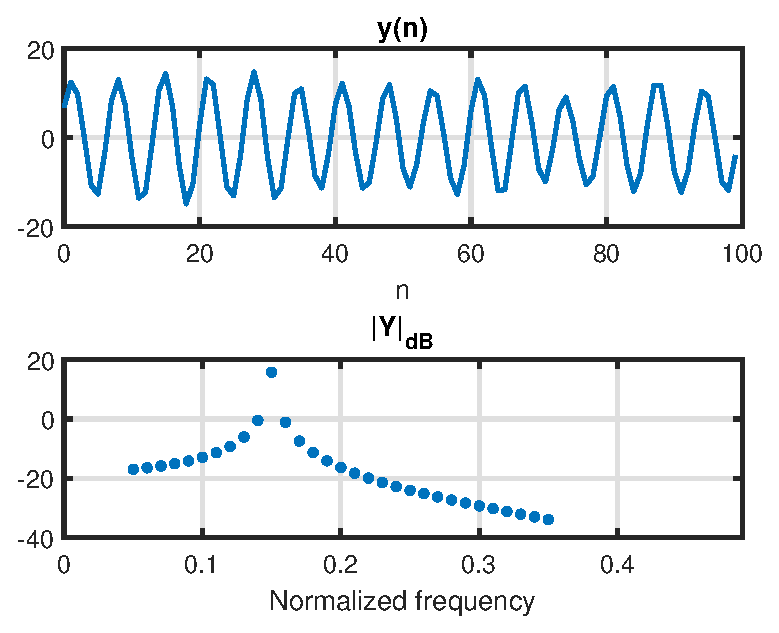
\includegraphics[width=0.65\textwidth]{figures/MS_y.eps}
    \caption{Output of the second-order system.}
    \label{fig:MS_y}
\end{figure}

\begin{figure}[H]
    \centering
    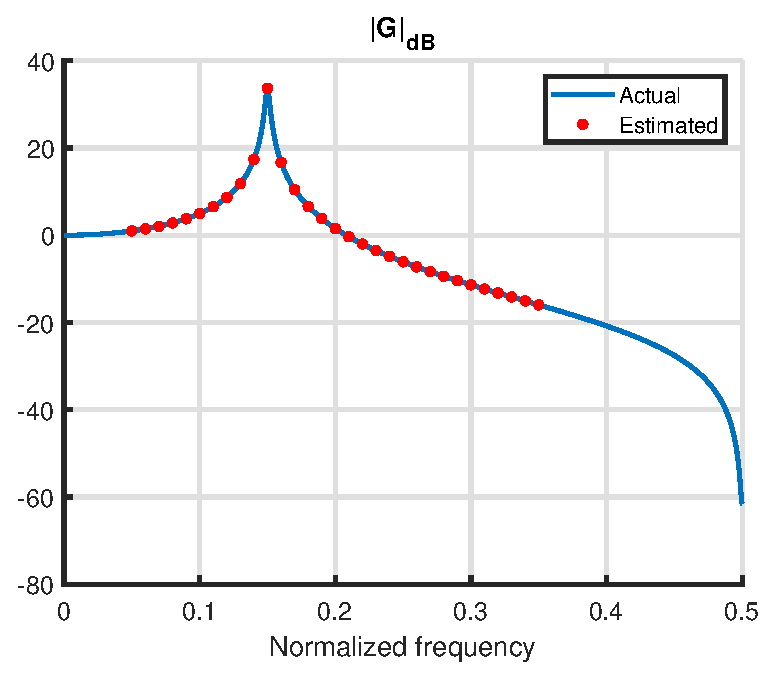
\includegraphics[width=0.65\textwidth]{figures/MS_G.eps}
    \caption{Magnitude FRF of the second-order system and the estimated FRF at the excited frequencies using (\ref{eq:G=Y/U_MS}).}
    \label{fig:MS_G}
\end{figure}

\newpage
\section{Measurement set-ups}
\subsection{Zero-order hold set-up}
In a lot of measurement set-ups, the input signal is generated digitally with a Zero-order hold (ZOH). This means that the signal is kept constant for a whole sampling period. At the sampling instants, a CT system $G(s)$ preceded by a ZOH can be modelled exactly as a DT system. \cite[eq. (34)]{ZOH_reference}
\begin{equation}
    G_{\mathrm{ZOH}}(z) = (1-z^{-1})  \mathcal{Z}\Big\{\mathcal{L}^{-1}\big\{\frac{G(s)}{s} \big\}\rvert_{t=n T_s}\Big\}
    \label{eq:ZOH_transform}
\end{equation}

The ZOH measurement set-up is shown in figure \ref{fig:zoh_setup}. In this case, the actuator $G_\mathrm{act}(s)$ is part of the FRF that is measured. The dynamics of the measurement device $G_y(s)$ must be calibrated perfectly ($G_y(s)=1)$ if one wants to measure the FRF from generator to output. Note that, in theory, the ZOH set-up is not allowed to contain anti-alias filters.
\begin{figure}[H]
    \centering
    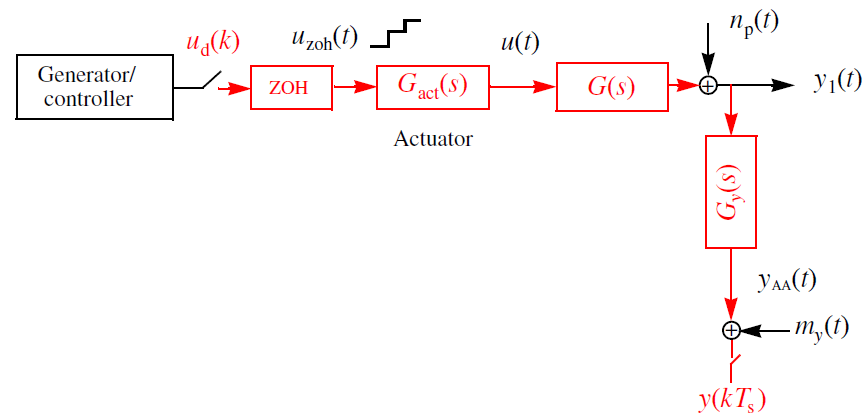
\includegraphics[width =0.65\textwidth]{figures/ZOH_setup.png}
    \caption{Zero-order hold measurement set-up. \textcolor{red}{Red} indicates which parts are modelled. Taken from \cite{identification_of_dynamical_sytems_slides}.}
    \label{fig:zoh_setup}
\end{figure}
Thus, if no anti-alias filter is used at the output and assuming that the actuator is perfect $G_{\textrm{act}}(s)=1$, when a CT system is excited with a ZOH and is sampled, we are actually measuring the ZOH version of the FRF and not the CT FRF directly. This is bad news if we want to measure the CT FRF $G(s)$. However, this can be circumvented. When $|f| \ll f_s/2$, there isn't a big difference between the CT FRF $G(s)$ and the ZOH version of $G(s)$.
\begin{equation}
    G(j 2 \pi f) \approx G_{\mathrm{ZOH}}(e^{j 2 \pi f T_s})
    \label{eq:Gzohapprox}
\end{equation}

So, when the goal is to measure a CT FRF with a ZOH set-up, care must be taken to stay within the region where this approximation holds. This can be accomplished by making sure that the highest excited frequency in the input signal is well below the sampling frequency of the measurement set-up.
\begin{equation*}
    f_{\text{max}} \ll f_s/2
\end{equation*}

\paragraph{Example}
Consider a second order system.
\begin{equation*}
    G(s) = \frac{\omega_0^2}{s^2 + 2 \zeta \omega_0 s + \omega_0^2} \text{ with } \omega_0 = 2 \pi 0.3 [\text{rad}/s] \text{ and } \zeta = 0.01
\end{equation*}
Applying the ZOH transformation (\ref{eq:ZOH_transform}) to this system with $f_s = 2 \text{Hz}$ results in the DT system that was used in previous examples (\ref{eq:Gz_example}). The magnitude FRF of both the CT system and the ZOH version of it are plotted in figure \ref{fig:Gzoh_example}. Notice that the DT system has a periodic FRF while the CT system does not. Moreover, at the low frequencies, both FRFs overlap. The approximation (\ref{eq:Gzohapprox}) is worse once the frequency gets close to $f_s/2$.

\begin{figure}[H]
    \centering
    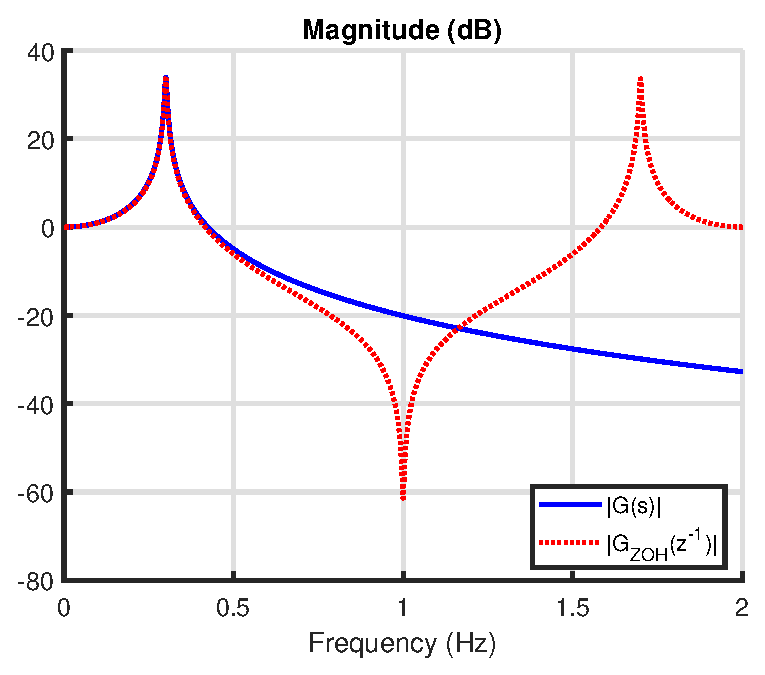
\includegraphics[width=0.65\textwidth]{figures/ZOH.eps}
    \caption{Magnitude FRF of the second-order system and the magnitude FRF of the ZOH version of it with $f_s = 2 \text{Hz}$.}
    \label{fig:Gzoh_example}
\end{figure}

\subsection{Band-limited set-up}
\label{sec:band-limited}
Even if one uses a high sampling frequency $f_s$, the actuator dynamics will still influence the measurement of the FRF when using a ZOH set-up. This is not an issue when a band-limited set-up is used. The band-limited set-up is shown in figure \ref{fig:BL_setup}. In a band-limited set-up, the input to the system can still be generated by a ZOH. But the input to the system must be measured and an anti-alias filter must be used to avoid aliasing. By measuring the input to the system, the dynamics of the actuator won't be part of the FRF estimate. The output of the system must also go through an anti-alias filter before being measured. A relative calibration is needed if one wants to measure the FRF from the input to the output. Concretely this means that the ratio of the anti-alias filters $G_y(s)/G_u(s)$ must be taken into account when processing the measurements.

\begin{figure}[H]
    \centering
    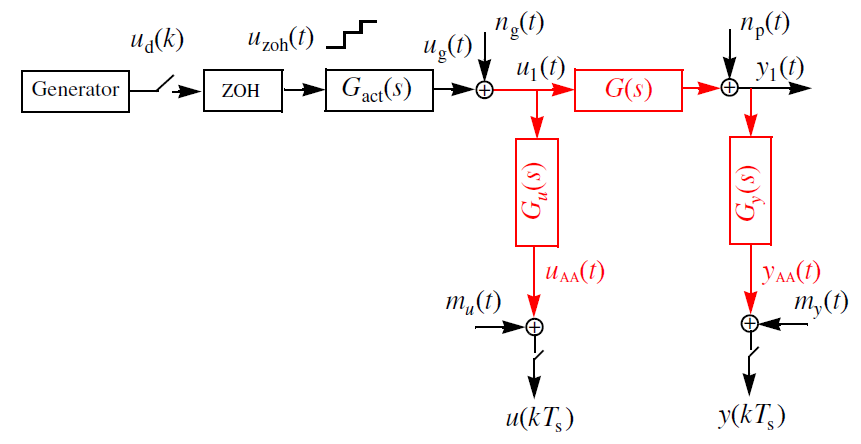
\includegraphics[width =0.65\textwidth]{figures/BL_setup.png}
    \caption{Band-limited measurement set-up. \textcolor{red}{Red} indicates which parts are modelled. Taken from \cite{identification_of_dynamical_sytems_slides}.}
    \label{fig:BL_setup}
\end{figure}


\section{System transients}
\label{sec:system_transients}
The first condition of perfect reconstructability (periodicity) implies that the signal has been repeating forever until now and will repeat forever in the future. This is not realistic; when a system is excited, the excitation must have started at some time in the past and must end at some point in the future. In the example of the previous section we had briefly mentioned that the measurements were taken in steady state. Concretely, the input was applied to the system for 20 periods and only the last period was used for the analysis, thereby ensuring that the system transients have faded away. This can be quantified by calculating the RMS of the difference between the output of the $p$-th period and the output of the last period. This is plotted in figure \ref{fig:MS_transients_RMS_error}. The RMS of the difference decreases exponentially. If the measurements were noisy, the RMS of the difference would decrease until the transients are below noise level, at which point the transients can be said to have faded away. In this case, the RMS of the difference reaches approximately $10^{-7}$ by the 20-th period, which is negligible for our purposes.

\begin{figure}[H]
    \centering
    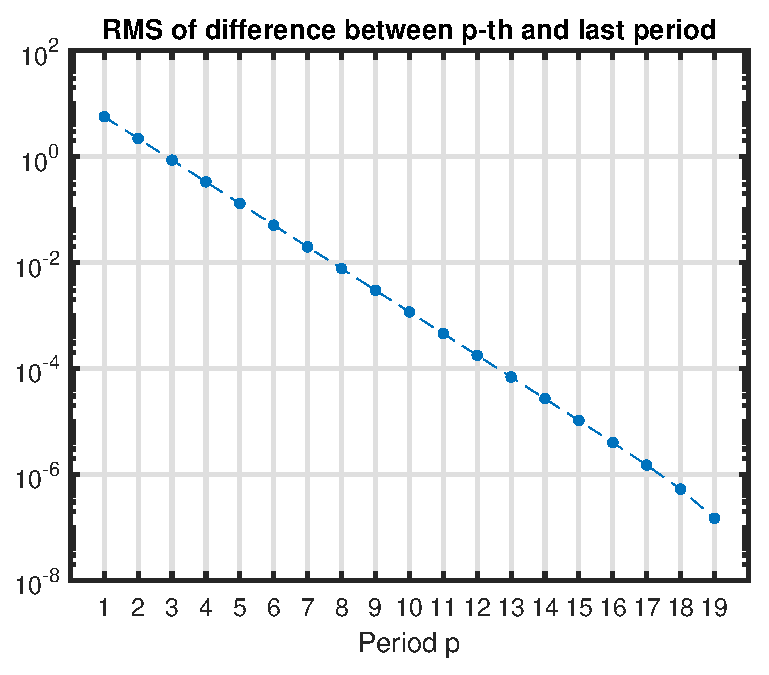
\includegraphics[width=0.65\textwidth]{figures/MS_transients_RMS_error.eps}
    \caption{RMS of the difference between the output of every period and the output of the last period.}
    \label{fig:MS_transients_RMS_error}
\end{figure}

It turns out that the transient term is just a rational function added on top of the steady state output spectrum.
\begin{equation}
\boxed{
    Y(k) = G(e^{-j 2 \pi k/N}) U(k) + T(k)
    }
    \label{eq:Y=GU+T}
\end{equation}
with
\begin{equation*}
    T(k) = \frac{I(e^{-j 2 \pi k/N})}{A(e^{-j 2 \pi k/N})}
\end{equation*}

$I(e^{-j 2 \pi k/N})$ is a polynomial in $e^{-j 2 \pi k/N}$ whose coefficients depend on the difference between samples from the previous period and samples from the current period. This is proven for DT systems in appendix \ref{appendix:transient_term}. The transient term for CT systems will be discussed afterwards.


If $u(n)$ and $y(n)$ are periodic, then $T(k)=0$, because $I(e^{-j 2 \pi k/N})$ only depends on the difference between the in- and output at the end of the current period and the in- and output at the end of the previous period. In this case (\ref{eq:Y=GU+T}) simplifies to what we had before.
\begin{equation*}
    Y(k) = G(e^{-j 2 \pi k/N}) U(k)
\end{equation*}

A key property of the transient term $T(k)$ is that it is a ``smooth'' function of the frequency $k$. This is due to the fact that it is a rational form of $e^{-j2\pi k/N}$. This property can be used to suppress the transient, as will be explained later. Another property of $T(k)$ is that its denominator is the same as the denominator of $G(e^{-j 2 \pi k/N})$. Therefore, the transient term will ``resemble'' the shape of the FRF.

\paragraph{CT transients}
Similar results can be derived for CT systems \cite{pintelon_book}.
\begin{equation*}
\boxed{
    Y(k) = G(j\omega)U(k) + T(k) + \delta(k)
    }
\end{equation*}
In this case, the numerator of $T(k)$ depends on the difference in initial conditions at $t=0$ and $t=T=n T_s$:
\begin{equation*}
    \Big[\frac{d^p y}{{dt}^p}(T) - \frac{d^p y}{{dt}^p}(0)\Big] \text{ and } \Big[\frac{d^p u}{{dt}^p}(T) - \frac{d^p u}{{dt}^p}(0)\Big]
\end{equation*}
with $p \in \mathds{N}$ and $p < \max{(n_a,n_b)}$, $n_a$ and $n_b$ being the order of the denominator and numerator of $G(s)$ respectively. An additional term $\delta(k)$ pops up. This is the alias error and it can be generated when the transient $T(j\omega)$ overextends into the aliasing frequencies  $f > f_s/2$. It is present even if the signals have been low-pass filtered. Because the alias error $\delta(k)$ is also smooth, it can be grouped together with the transient term $T(k)$.


\newpage
\paragraph{Example}
Again, the same second-order system (\ref{eq:Gz_example}) of the previous section is used. This time we will take a look at the estimation error.
\begin{align*}
    G_{\mathrm{est}}(e^{-j 2 \pi k/N}) - G(e^{-j 2 \pi k/N}) &= \frac{Y(k)}{U(k)} - G(e^{-j 2 \pi k/N}) \\ &=  \frac{G(e^{-j 2 \pi k/N}) U(k) + T(k)}{U(k)} - G(e^{-j 2 \pi k/N}) \\ &=  \frac{T(k)}{U(k)}
\end{align*}
As the magnitude spectrum of $u(n)$ is flat, the magnitude of the estimation error will be proportional to the magnitude of the transient term.

The estimation error for the FRF estimated from the first and 20th period is shown in figure \ref{fig:MS_G_transients}. The error of the FRF calculated from the last period is around $-150 \text{dB}$, which is negligible. In other words, there is no transient term as the system is in steady state. The error for the first period is a smooth function of the frequency and ``resembles'' the shape of the transfer function as expected.

\begin{figure}[H]
    \centering
    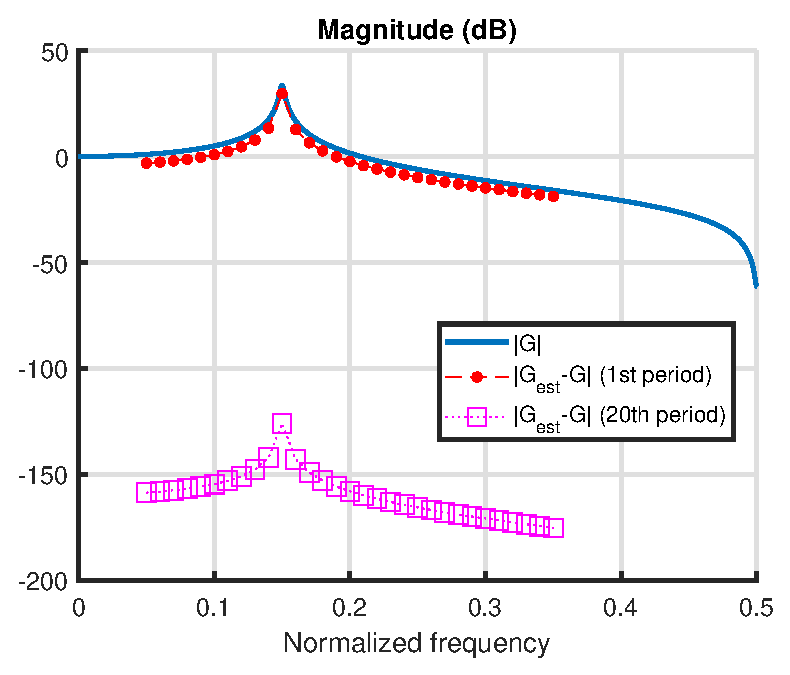
\includegraphics[width=0.65\textwidth]{figures/MS_G_transients.eps}
    \caption{Magnitude FRF of the second-order system and the estimation errors of the FRF at the excited frequencies using (\ref{eq:G=Y/U_MS}) for the data from the first period and the 20th period.}
    \label{fig:MS_G_transients}
\end{figure}

\section{Frequency domain methods}
Till now we have been treating CT and DT systems as separate cases. However, FD methods can be generalized to both CT and DT systems. There is no reason why a FD method should only work for one and not the other. To generalize these methods it is useful to define $\Omega$ to encompass both CT and DT models. $\Omega$ can either be $s$ or $z^{-1}$.
\begin{equation*}
    \Omega = \begin{cases}
        s & \text{if working in continuous-time (CT)} \\
        z^{-1} & \text{if working in discrete-time (DT)} 
    \end{cases}
\end{equation*}
Thus, denoting an LTI system as $G(\Omega)$ is not specific to CT or DT systems. When the FRF is evaluated in the DFT frequencies $\omega_k = 2 \pi k f_s/N$ it, is denoted $\Omega_k$.
\begin{equation*}
    \Omega_k = \begin{cases}
        j \omega_k = j 2 \pi k f_s/N& \text{if working in continuous-time (CT)} \\
        e^{-j \omega_k T_s} = e^{-j 2 \pi k/N} & \text{if working in discrete-time (DT)} 
    \end{cases}
\end{equation*}

\section{White noise}
\label{sec:white_noise}
White noise is a random signal with a flat power spectrum. A zero-mean Gaussian sequence is white noise.
\begin{equation*}
    v(n) \sim \mathcal{N}(0,\sigma^2)
\end{equation*}
Let's assume that a measurement is perturbed by this white noise.
\begin{equation*}
    x(n) = x_0(n) + v(n)
\end{equation*}
Due to the linearity of the DFT one obtains
\begin{equation*}
    X(k) = X_0(k) + V(k)
\end{equation*}
Thus it is interesting to understand the properties of the DFT of this white noise sequence.
\begin{equation*}
    V(k) = \frac{1}{N}\sum_{n=0}^{N-1} v(n) e^{-j 2\pi k n/N}
\end{equation*}
It turns out that (see appendix \ref{appendix:white_noise})
\begin{align*}
    &\mathbb{E}\{V(k)\} = 0\\
    &\mathbb{E}\{|V(k)|^2\} = \frac{1}{N} \sigma^2 \\
    &\mathbb{E}\{V^2(k)\} = 0 \text{ if mod}(2k,N) \neq 0
\end{align*}

\section{Periodic signals}
What happens to the DFT spectrum when we apply a signal periodically? Let's assume that we have a sequence $\tilde{x}(n)$ of length $N$ with corresponding DFT
\begin{equation*}
    \tilde{X}(k) = \sum_{n=0}^{N-1} \tilde{x}(n) e^{-j 2\pi k n/N}
\end{equation*}
Now, the sequence $\tilde{x}(n)$ will be repeated one more time to obtain a sequence of length $2N$.
\begin{equation*}
    x(n) = \begin{cases}
        \tilde{x}(n) &\text{ if } 0 \leq n < N - 1\\
        \tilde{x}(n-N) &\text{ if } N \leq n < 2N - 1
    \end{cases}
\end{equation*}
The DFT of $x(n)$ is then given by
\begin{align*}
    X(k) &= \frac{1}{2N}\sum_{n=0}^{2 N-1} \tilde{x}(n) e^{-j 2\pi k n/(2N)} = \frac{1}{2N}\sum_{n=0}^{N-1} \tilde{x}(n) e^{-j 2\pi k n/(2N)} + \frac{1}{2N}\sum_{n=N}^{2N-1} \tilde{x}(n-N) e^{-j 2\pi k n/(2N)} \\
    &= \frac{1}{2N}\sum_{n=0}^{N-1} \tilde{x}(n) e^{-j 2\pi k n/(2N)} + \frac{1}{2N}\sum_{n=0}^{N-1} \tilde{x}(n) e^{-j 2\pi k n/(2N)}  e^{-j 2\pi k/2} \\
    &= \frac{1}{N}\sum_{n=0}^{N-1} \tilde{x}(n) e^{-j 2\pi k n/(2N)} \frac{1+e^{-j 2\pi k/2}}{2}
    \end{align*}
Evaluating this in $2k$ and $2k+1$ gives
\begin{align*}
    &X(2k) = \tilde{X}(k)\\
    &X(2k+1) = 0
\end{align*}
Thus, the even DFT lines will contain the information of $X(k)$ and the odd DFT lines will be zero.

This result can be generalized to a signal that is repeated $P$ times.
\begin{equation*}
\boxed{
    %x(n) = \tilde{x}(\text{mod}(n,P)) \Rightarrow 
    X(kP+r) =
    \begin{cases}
        \tilde{X}(k) &\text{ if } r = 0\\
        0 & \text{ if } r = 1,\ldots,P-1\\
    \end{cases}
}
\end{equation*}

\newpage
\paragraph{Example}
A random phase multisine ($N=40$) is created where the 3 lowest DFT bins are excited with an RMS value of 1. This signal is repeated $P=3$ times. The repeated signal is plotted in the TD and the FD in figure \ref{fig:periodic_MS}. It can be seen that in the periodic signal there are $P-1 = 2$ non-excited lines in between the excited lines.

\begin{figure}[H]
    \centering
    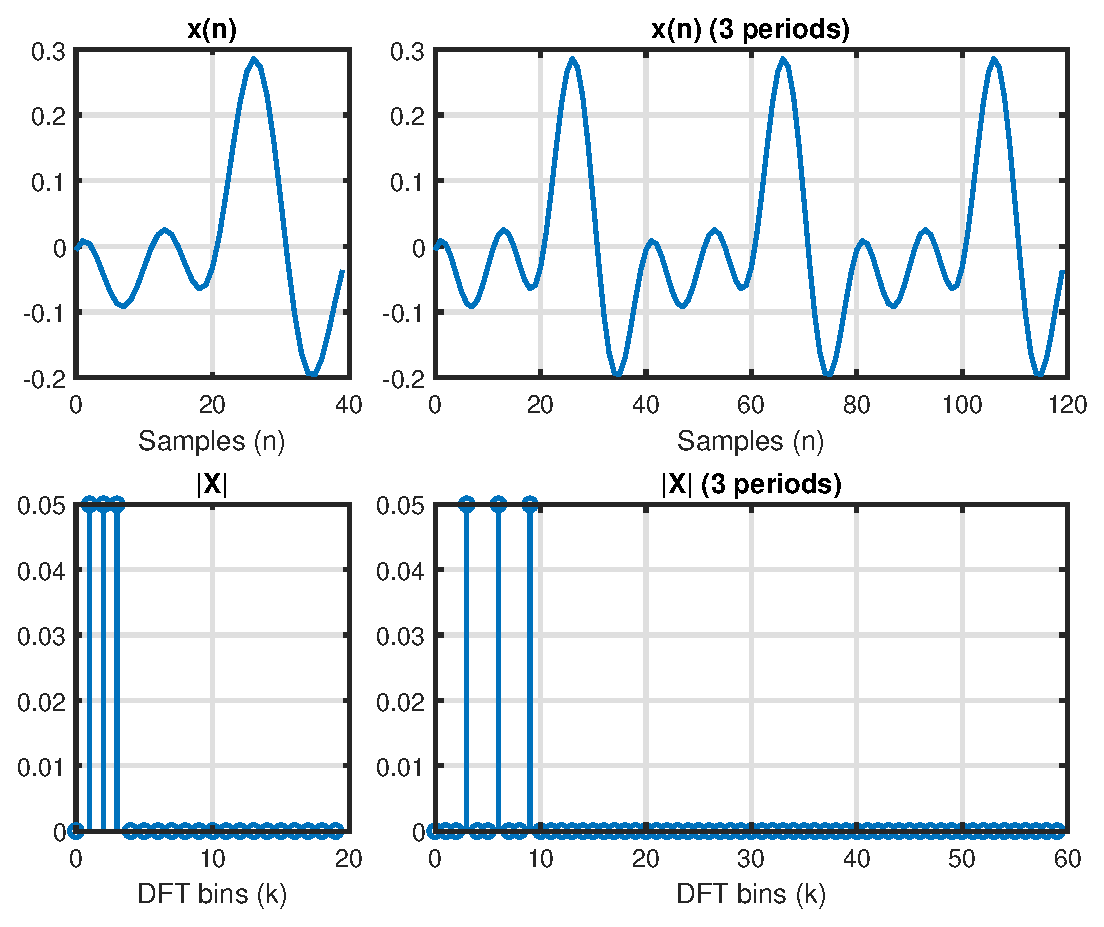
\includegraphics[width = 0.65\textwidth]{figures/periodic.eps}
    \caption{A multisine is repeated 3 times.}
    \label{fig:periodic_MS}
\end{figure}


\section{Transient suppression}
In section \ref{sec:system_transients} it was shown that transients in the output will negatively impact the quality of the FRF estimate. However, there are multiple ways to suppress these transients. The most obvious way is to wait for the system to enter steady state and to only start measuring once the transients have faded away. This is exactly what was done in the example of section \ref{sec:system_transients} (see figure \ref{fig:MS_G_transients}). There are also ways to suppress the transient without throwing away the measurements that are not in steady state. 3 of them will be discussed:
\begin{itemize}
    \item Windowing
    \item Parametric estimation
    \item The local polynomial method
\end{itemize}

\newpage
\subsection{Windowing}
There are many possible windows that one can choose from. The Hann window is a popular one.
\begin{equation}
    w(n) = \frac{1}{2} [1 - \cos(\frac{2\pi n}{N})] \,,\quad n = 0,\ldots,N-1
\end{equation}
The windowed input and output are then given by
\begin{equation*}
    u_w(n) = w(n) u(n) \text{ and } y_w(n) = w(n) y(n)
\end{equation*}
A multiplication in the TD becomes a convolution in the FD.
\begin{equation*}
    U_W(k) = W(k) * U(k) \text{ and } Y_W(k) = W(k) * Y(k) 
\end{equation*}
with $W(k) = \frac{1}{2} \delta(k) - \frac{1}{4} \delta(k+1) - \frac{1}{4} \delta(k-1)$.
The windowed estimate of the FRF is then given by
\begin{equation}
    G_W(\Omega_k) = \frac{Y_W(k)}{U_W(k)}
    \label{eq:G_W}
\end{equation}

Let's now see why windowing will reduce the effect of the transient.
\begin{equation*}
    Y_W(k) = W(k) * (G(\Omega_k) U(k) + T(k))
\end{equation*}
For the first term the following approximation can be made:
\begin{equation*}
    W(k) * [G(\Omega_k) U(k)] \approx G(\omega_k) [W(k) * U(k)] = G(\omega_k) U_W(k)
\end{equation*}
Hereby it is assumed that $G(\Omega_{k-1}) \approx G(\Omega_{k}) \approx G(\Omega_{k+1})$. In other words, $G(\Omega)$ is flat around $\Omega_k$. (\ref{eq:G_W}) then becomes
\begin{equation*}
    G_W(\Omega_k) \approx G(\Omega_k) + \frac{T_W(k)}{U_W(k)}
\end{equation*}
The trick now is to use the property that $T(k)$ is a smooth function of the frequency. Let's assume that $T(k)$ can be captured locally by a second order polynomial.
\begin{equation*}
    T(k) = a k^2 + b k + c
\end{equation*}
Windowing $T(k)$ gives
\begin{equation*}
    T_W(k) \propto 2 T(k) - T(k+1) - T(k-1) = - 2 a
\end{equation*}
This is a bit like taking the second order derivative, which suppresses the transient.

\newpage
\paragraph{Example}
The DT system (\ref{eq:Gz_example}) is taken again. The same input as in figure \ref{fig:MS_u} is used. The estimation error of the FRF with and without windowing is shown in figure \ref{fig:hann_window_FRF}. Windowing gives better results, except near the resonance frequency. This is because the approximation that $G(\Omega)$ is flat does not hold in this region.
\begin{figure}[H]
    \centering
    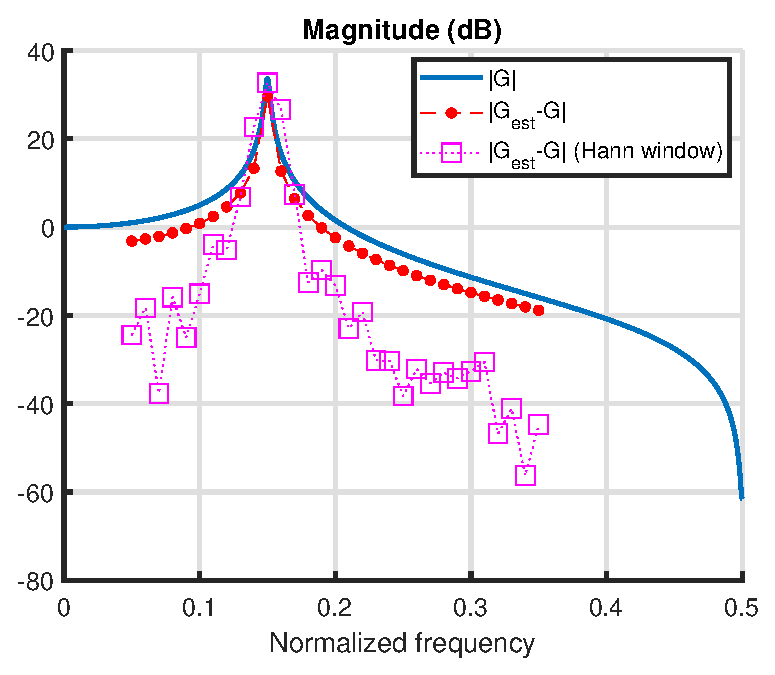
\includegraphics[width =0.65 \textwidth]{figures/hann_window.eps}
    \caption{Comparison of FRF estimation error without and with Hann windowing.}
    \label{fig:hann_window_FRF}
\end{figure}


\subsection{Parametric estimation}
Till now, only nonparametric estimates of the FRF were discussed. Unlike line-fitting, where one is interested in the slope and offset of the line, the nonparametric estimate does no such thing. The result of the nonparametric estimate is the FRF estimate at every excited frequency. However, in a sense there are still parameters: these are the FRF estimates at every frequency bin $k \in \kexc$.

The TF of the system is however still given by a rational function. The coefficients of this rational function can be estimated. The transient term is also a rational function and the parameters describing it can also be included in the estimation.
\begin{equation*}
    Y(k) = G(\Omega_k) U(k) + T(k)
\end{equation*}
Using $G(\Omega_k) = \frac{B(\Omega_k)}{A(\Omega_k)}$ and $T(k) = \frac{I(\Omega_k)}{A(\Omega_k)}$ the expression above can be rewritten as
\begin{equation}
    A(\Omega_k) Y(k) - B(\Omega_k) U(k) - I(\Omega_k) = 0
    \label{eq:AY-BU-I=0}
\end{equation}
$A(\Omega_k)$ is a polynomial of order $n_a$ and $B(\Omega_k)$ is a polynomial of order $n_b$. (\ref{eq:I_explicit}) in appendix \ref{appendix:transient_term} is an explicit formula for $I(\Omega_k)$. From this formula, it can be verified that $I(\Omega_k)$ is a polynomial of order $n_I$ with
\begin{equation*}
    n_I = \max{(n_a,n_b)}-1
\end{equation*}
For CT systems, there is also an alias error on top of the transient term. These errors can also be captured well by a polynomial. Grouping the alias error together with the $I(\Omega_k)$ results in \cite[Section 6.3.2.3]{pintelon_book}
\begin{equation*}
    n_I \geq \max{(n_a,n_b)}
\end{equation*}
After a bit of calculations, (\ref{eq:AY-BU-I=0}) can be turned into
\begin{equation*}
    \begin{bmatrix}
    \vdots & & \vdots & \vdots & & \vdots & \vdots & & \vdots \\
    Y(k) & \hdots & Y(k) \Omega_k^{n_a} & 
    U(k) & \hdots & U(k) \Omega_k^{n_b} & 
    1    & \hdots &      \Omega_k^{n_I} \\
    \vdots & & \vdots & \vdots & & \vdots & \vdots &  & \vdots
    \end{bmatrix}
    \begin{bmatrix}
    a_0 \\ \vdots \\ a_{n_a} \\ 
    -b_0 \\ \vdots \\ -b_{n_b} \\
    -i_0 \\ \vdots \\ -i_{n_I}
    \end{bmatrix} = 0
\end{equation*}
This can be solved by calculating the right null-space of the first matrix. The coefficients $i_p$ will capture the transient. Note that the null space is empty if the measurements are noisy. We won't go into these details in this work, so the interested reader is referred to \cite{markovsky_book}.

\paragraph{Example}
Again, the DT system (\ref{eq:Gz_example}) is used with the same input shown in figure \ref{fig:MS_u}. The parameters are determined as described above. The resulting FRF estimation error is plotted in figure \ref{fig:transient_parametric}. Note that as a parametric representation is obtained, the FRF can be calculated at all frequencies. The error is around $-300 \text{dB}$, which is MATLAB's precision. This means that the error is negligible and that the transient has been fully suppressed.

\begin{figure}[H]
    \centering
    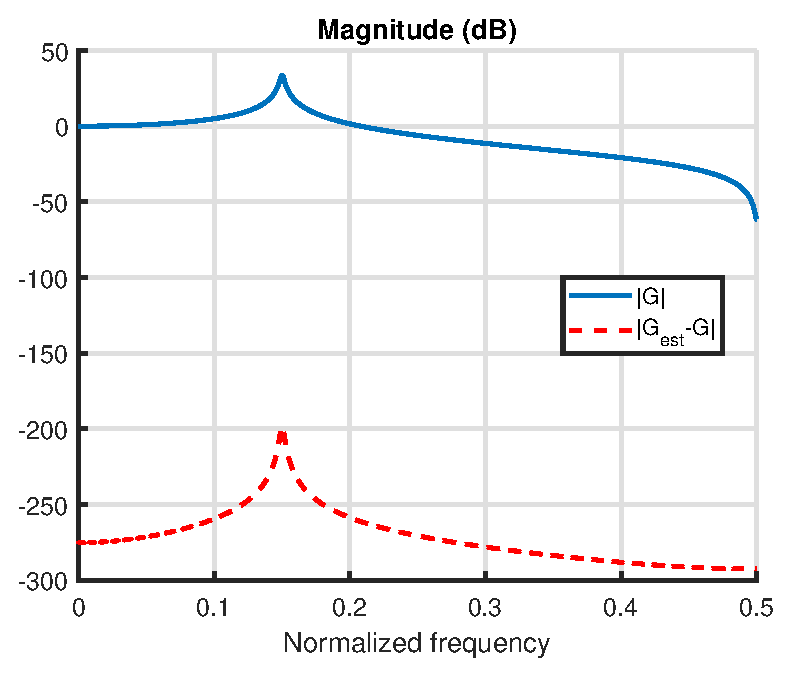
\includegraphics[width=0.65\textwidth]{figures/parametric_transient.eps}
    \caption{FRF estimation error for the parametric estimation of the TF with transient terms.}
    \label{fig:transient_parametric}
\end{figure}


\section{Local polynomial method}
\label{sec:LPM}
The idea of the local polynomial method (LPM) is quite simple. There are multiple variants of the LPM, but here we will focus on the robust LPM for periodic excitations. More information about all the variants of the LPM can be found in \cite[Chapter 7]{pintelon_book}.

\subsection{Response of a system excited by a periodic input}
For the robust LPM for periodic signals to work, at least $P=2$ periods must be measured. Let's assume for the sake of simplicity that the input $\tilde{u}(n)$ is noiseless and in steady state. $\tilde{u}(n)$ is applied $P$ consecutive times to the system.
%\begin{equation*}
%    u(n) = \tilde{u}(\text{mod}(n,P)) \,,\quad n = 0,1,\ldots,N P-1
%\end{equation*}
The spectrum of the input $u(n)$ is
\begin{equation}
    U(kP+r) =  
    \begin{cases}
        \tilde{U}(k) &\text{ if } r = 0\\
        0 & \text{ if } r = 1,\ldots,P-1
    \end{cases}
    \label{eq:U(kP+r)}
\end{equation}
It will resemble the spectrum shown in figure \ref{fig:periodic_MS}. Assuming that the output is perturbed by additive noise, the output spectrum is given by
\begin{equation*}
    Y(kP+r) = G(kP+r)U(kP+r) + T(kP+r) + N_y(kP+r)
\end{equation*}
$T(kP+r)$ is the transient term that arises from the fact that the system might not be in steady state. $N_y(kP+r)$ is additive noise that is added to the output. It can either be white noise (see section \ref{sec:white_noise}) or filtered white noise. Using (\ref{eq:U(kP+r)}), we can be more specific about the output spectrum.
\begin{equation*}
\boxed{
    Y(kP+r) =
    \begin{cases}
     G(kP)U(kP) + T(kP) + N_Y(kP) &\text{ if } r = 0\\
     T(kP+r) + N_Y(kP+r) &\text{ if } r = 1,\ldots,P-1
     \end{cases}
     }
\end{equation*}

\paragraph{Example}
The system (\ref{eq:Gz_example}) is excited with the signal shown in figure \ref{fig:periodic_MS}. The output is perturbed by Gaussian white noise with a standard deviation of 0.005. The input and output spectra are plotted in figure \ref{fig:periodic_output}. The output spectrum at the DFT lines 3, 6 and 9 are dominated by the $G(kP)U(kP)$ term. There is a peak around the 18-th DFT line that corresponds to the transient term $T$. The 18-th DFT line corresponds to the normalized frequency $18/(NP) = 18/120 = 0.15$, which corresponds to the normalized resonance frequency of the system (see figure \ref{fig:transient_parametric} for example). This is to be expected as the transient resembles the shape of the transfer function. Finally, after the 30-th DFT bin, the noise terms $N_Y$ dominate the output.

\begin{figure}[H]
    \centering
    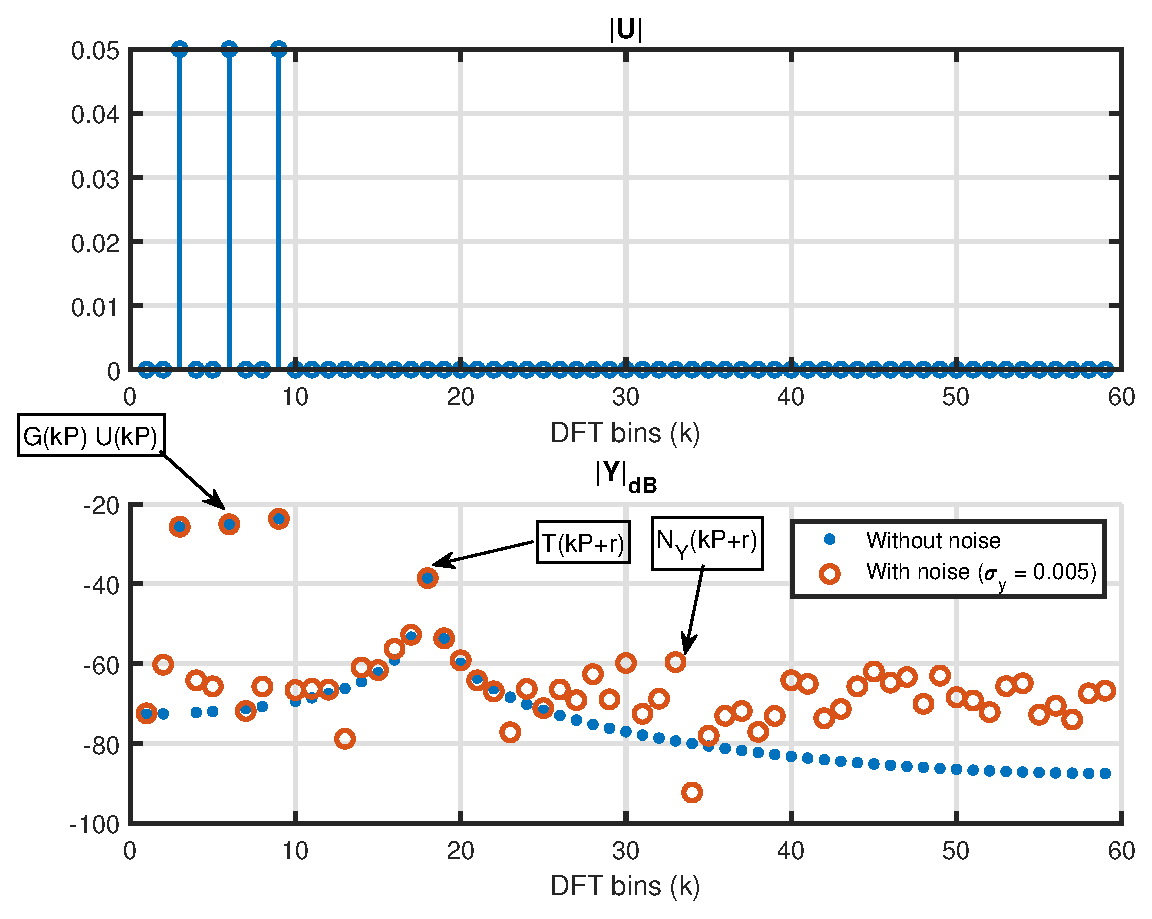
\includegraphics[width = 0.65\textwidth]{figures/periodic_output.eps}
    \caption{Input and output of the DT system (\ref{eq:Gz_example})}
    \label{fig:periodic_output}
\end{figure}

\subsection{Algorithm} Now we can finally discuss the algorithm of the robust LPM. The idea is to estimate the contribution of the transient term at the excited frequencies using the data at the non-excited frequencies. To this end, we will work in a window around every excited DFT bin. In the case of the previous example, the excited bins are k = 1, 2 and 3. Two parameters must be chosen by the user. The first one is the window size $2n$. We must use $n$ unexcited bins before and after $kP$. 

\paragraph{Example}
$k = 3$, $P=3$, $n=4$. We are working in a window around $Y(kP) = Y(9)$. We must use 4 unexcited bins before and after 9.
\begin{equation*}
    Y(9+r_i) \text{ with } r_i = -5,-4,-2,-1,1,2,4,5
\end{equation*}
For every one of the unexcited lines the following holds
\begin{equation*}
    Y(kP+r_i) = T(kP+r_i) + N_Y(kP+r_i)
\end{equation*}
The transient term can be modelled as a polynomial of $r$. This is because the transient is a smooth function of the frequency. The order of the polynomial $R$ is the second parameter that the user can choose.
\begin{equation*}
    T(kP+r) \approx T(kP) + \sum_{s=1}^R t_s(k) r^s
\end{equation*}
We can then find the polynomial of best fit through the points $Y(kP+r_i)$

\paragraph{Example continued}
Putting all the $Y(9+r_i)$ into a vector and choosing $R=2$ gives
\begin{equation*}
    \begin{bmatrix}
    Y(4)\\Y(5)\\Y(7)\\Y(8)\\Y(10)\\Y(11)\\Y(13)\\Y(14)
    \end{bmatrix} = 
    \begin{bmatrix}
    1 & (-5) & (-5)^2 \\
    1 & (-4) & (-4)^2 \\
    1 & (-2) & (-2)^2 \\
    1 & (-1) & (-1)^2 \\
    1 & 1 & 1^2 \\
    1 & 2 & 2^2 \\
    1 & 4 & 4^2 \\
    1 & 5 & 5^2 \\
    \end{bmatrix}
    \begin{bmatrix}
    T(9) \\ t_1(3) \\ t_2(3)
    \end{bmatrix} + 
    \begin{bmatrix}
    N_Y(4)\\N_Y(5)\\N_Y(7)\\N_Y(8)\\N_Y(10)\\N_Y(11)\\N_Y(13)\\N_Y(14)
    \end{bmatrix}
    \longrightarrow
    Y_n = K_n \Theta + V_n
\end{equation*}
The least squares solution is given by\footnote{Note that calculating the solution like this results in an ill-conditioned problem. The \textbackslash \ operator in MATLAB solves this problem using QR-factorisation, which is better conditioned. ($\theta = K_n \backslash Y_n$)}
\begin{equation*}
    \hat{\Theta} = (K_n^H K_n)^{-1}K_n^H Y_n
\end{equation*}
This results in an estimation of the transient term at the excited DFT bin $\hat{T}(9)$. The other terms $t_1(3)$ and $t_2(3)$ are not important.

Finally, the estimated transient term can be removed from the output spectrum at the excited DFT line.
\begin{equation*}
\boxed{
    \hat{Y}(kP) = Y(kP) - \hat{T}(kP)
}
\end{equation*}
Thus, the transient has been suppressed. The FRF can then be calculated simply as
\begin{equation*}
    \hat G(\Omega_k) = \frac{\hat{Y}(kP)}{U(kP)}
\end{equation*}
The entire procedure outlined here must be repeated for all $k \in \kexc$.

\subsection{Variance estimate}
Having a variance estimate of the output spectrum is useful for providing uncertainty bounds. It can also be used as a nonparametric weighting in parametric identification of the system transfer function. %\cite[Introduction]{nonparametric_periodic}

The residual is defined as the difference between the measured output spectrum and the predicted output spectrum.
\begin{equation*}
    \hat{V}_n = Y_n - K_n \hat{\Theta}
\end{equation*}
Assuming that the variance of the noise is white (flat) in the window $2n$, it can be used to estimate the variance at every $k \in \kexc$.
\begin{equation*}
    \hat\sigma^2_{\hat Y}(kP) = \frac{1}{q^{\text{noise}}} V_n^H V_n \,,\quad \text{ with } q^{\text{noise}} = 2 n - (R + 1) \text{ (degrees of freedom)}
\end{equation*}
A proof of this is given in appendix \ref{appendix:cov_est} and is based on \cite[Appendix 7.B]{pintelon_book}. The reason why we must divide by the degrees of freedom $q^{\text{noise}}$ and not by $2n$ is because $R+1$ parameters are estimated. This is analogous to the reason why the unbiased sample variance is calculated by dividing by the number of observations minus 1 when the population mean is also estimated. 

As $\hat G(\Omega_k) = \hat{Y}(kP)/U(kP)$, the variance of the FRF can be calculated as
\begin{equation}
    \hat\sigma^2_{\hat G}(\Omega_k) = \frac{\hat\sigma^2_Y(kP)}{|U(kP)|^2}
    \label{eq:variance_estimate_no_input_noise}
\end{equation}

\newpage
\subsection{Example}
The robust LPM is applied to measurements from the system (\ref{eq:Gz_example}). This time $N = 16384$ and $P=2$. The first $F=5000$ frequencies are excited with a random phase multisine with an RMS value 1. White Gaussian noise is added to the output with $\sigma_y = 0.2$. This corresponds to a signal-to-noise ratio (SNR) of $29.5 \mathrm{dB}$. This number is calculated as follows.
\begin{equation*}
    \mathrm{SNR}_{\mathrm{dB}} = 10 \log_{10} \Big ( \frac{\frac{1}{NP}\sum_{t=0}^{NP-1}y_0(t)^2}{\sigma_y^2} \Big ) = 29.5 \mathrm{dB}
\end{equation*}
The numerator is the mean of the squares of the noiseless output $y_0$ and the denominator is the power of the noise. The SNR is quite high as a consequence of the resonance that is present in the transfer function. 100 noise realizations are simulated while keeping the same random phase multisine as an input and the root-mean square (RMS) error is calculated to get an idea of the effectiveness of the estimator.
\begin{equation*}
    \text{RMS}[|\hat G - G|](\Omega_k) = \sqrt{\frac{1}{100}\sum_{i=1}^{100}|\hat G^{(i)}(\Omega_k)-G(\Omega_k)|^2} 
\end{equation*}
with $\hat G^{(i)}(\Omega_k)$ being the nonparametric estimate of $G(\Omega_k)$ for the $i$-th noise realization. The parameters used for the LPM are $R=2$, $n = 6$ which results in $q^{\text{noise}} = 9$ degrees of freedom. To make the results more presentable, the data points are taken together in windows of size 50 and are averaged. The results are shown in figure \ref{fig:LPM_example}. Not taking the transient into account is significantly worse around the resonance frequency of the system. The transient resembles the FRF of the system, which is why the error is most pronounced around the resonance frequency. However, far away from the resonance frequency, not taking the transient into account is approximately 1 dB better than using the Robust LPM. This is because the transient term is below the random noise contribution. LPM uses a noisy estimate of the transient and this estimate is subtracted from the output spectrum, leading to an increased variance. Finally, the robust LPM seems to be slightly better than windowing in this simulation.


\begin{figure}[H]
    \centering
    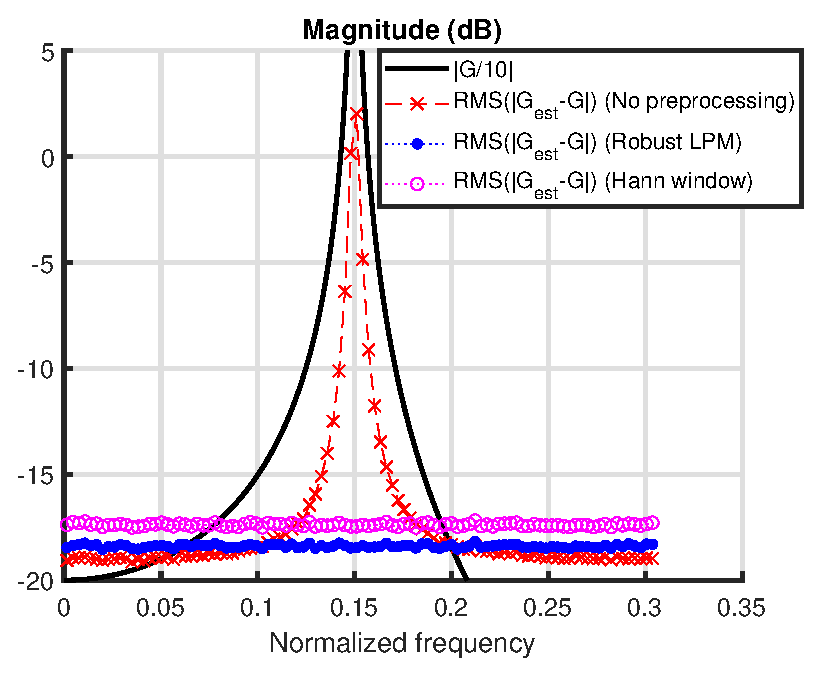
\includegraphics[width = 0.65\textwidth]{figures/LPM_example.eps}
    \caption{Comparison of the RMS error for the nonparametric estimate acquired without preprocessing, with windowing and with the robust LPM. $R=2$, $n = 6$, $q^{\text{noise}} = 9$.}
    \label{fig:LPM_example}
\end{figure}

\subsection{Choice of the order and degrees of freedom}
\label{sec:choice_order_dof}
Two parameters can be chosen by the user when performing the robust LPM analysis: the order of the polynomial approximation and the degrees of freedom used to estimate the noise variance.

\paragraph{Order}
A good way to choose the order is to start at $R=2$ and increment it in steps of two until the estimate of the variance $\hat \sigma^2_{\hat G}$ stops decreasing.

\paragraph{Degrees of freedom}
Increasing the degrees of freedom $q^{\text{noise}}$ will increase the window size $2n$. This gives a better estimation of the variance. There is a trade-off however: it was assumed that the noise variance is white (flat) in the window $2n$. Thus, making the window size too big will result in a loss of frequency resolution. Additionally, making the window size $2n$ bigger means that the transient is approximated by a polynomial over a larger window. At that point it might be necessary to increase the order $R$ of the polynomial.

\section{Generalization}
Many things were simplified until now. A few of the assumptions that were made are:
\begin{itemize}
    \item The input is noiseless.
    \item White Gaussian noise noise was simulated in the example, but what if the noise is filtered white noise?
    \item There is no feedback from output to input.
    \item The input is a multisine. What about random excitations?
\end{itemize}
Each of these points will be discussed briefly.

\subsection{Noisy input}
Of course, the measurement of the input can be noisy. Thankfully, the robust LPM is also able to estimate the input noise variance for periodic excitations. Given that the input is not known perfectly, the estimate of the FRF variance (\ref{eq:variance_estimate_no_input_noise}) is not correct any more. In general, the variance of an FRF estimate $\hat G(\Omega_k)$ can be approximated by
\begin{equation*}
    \hat \sigma_{\hat G}^2(k) = |\hat G(\Omega_k)|^2 \Bigg(\frac{\hat{\sigma}_{Y}^2(k)}{|\hat{Y}(k)|} + \frac{\hat{\sigma}_{U}^2(k)}{|\hat{U}(k)|}
-2\mathrm{Re}\left(\frac{\hat{\sigma}^2_{YU}(k)}{Y(k)\overline{U(k)}}\right) \Bigg)
\end{equation*}

The equation above is only applicable when the excitation is periodic and when the FRF is estimated by dividing the output spectrum $Y(k)$ by the input spectrum $U(k)$. It is also possible to estimate the variance of the noise for arbitrary excitations, but different formulas must be used \cite[Section 2.6]{pintelon_book}.

\subsection{Filtered white noise}
For simplicity sake, filtered white noise at the sampling instants is defined as
\begin{equation*}
    v(n) = S(z^{-1}) e(n) \,,\quad \text{ with } e(n) \sim \mathcal{N}(0,\sigma^2)
\end{equation*}
The power spectrum of this noise is not flat. This also means that the noise samples can be correlated over time.
\begin{equation*}
    \exists n,m \text{ with } n \neq m \text{ such that } \mathbb{E}\{v(n) v(m)\} \neq 0 
\end{equation*}
An important consequence of filtered white noise is that there will also be noise transients in the measurements.
\begin{equation*}
    V(k) = S(\Omega_k) E(k) + T_S(\Omega_k)
\end{equation*}
As the input of the noise filter is random, the noise transients will never fade away. This means that when one waits long enough for the system $G(\Omega)$ to enter steady state, there will still be noise transients in the measurements. This is where the LPM can also be useful.

\subsection{Feedback}
\label{sec:feedback}
Consider the measurement set-up shown in figure \ref{fig:neg_feedback_system}. An LTI system $G(z^{-1})$ is in negative feedback and the output is perturbed by process noise.

\begin{figure}[H]
    \centering
    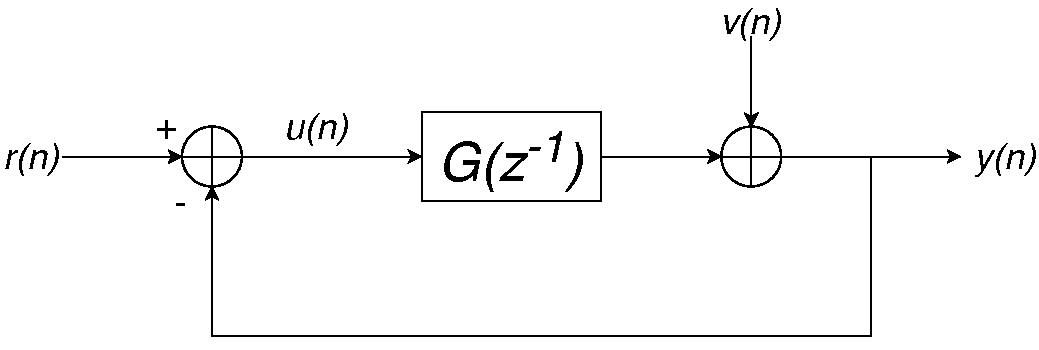
\includegraphics[width = 0.65\textwidth]{figures/system.pdf}
    \caption{LTI system in negative feedback with additive process noise.}
    \label{fig:neg_feedback_system}
\end{figure}

The Z-transform of the output and input are given by
\begin{align*}
    &Y(z) = \frac{G}{1+G} R(z) + \frac{1}{1+G} V(z)\\
    &U(z) = \frac{1}{1+G} R(z) - \frac{1}{1+G} V(z)
\end{align*}
Noise that affects the output also affects the input due to the feedback. Two possibilities will be considered: $r(n)$ is a multisine and $r(n)$ is a random signal. Assuming that the process noise $v(n)$ is a Gaussian white noise sequence with variance $\sigma_v^2$ we get
\begin{equation*}
    \mathbb{E}\{V(k)\} = 0 \text{ and } \mathbb{E}\{|V(k)|^2\} = \sigma_v^2(k)/N
\end{equation*}

\paragraph{$\boldsymbol{r(n)}$ is a multisine}
In this case we can apply multiple periods $P$ to the system. It is assumed that enough time has passed for the system transient to fade away and the noise transients will be neglected.
\begin{align*}
    &Y^{(p)}(k) = \frac{G(\Omega_k)}{1+G(\Omega_k)} R^{(p)}(k) + \frac{1}{1+G(\Omega_k)} V^{(p)}(k)\\
    &U^{(p)}(k) = \frac{1}{1+G(\Omega_k)} R^{(p)}(k) - \frac{1}{1+G(\Omega_k)} V^{(p)}(k)
\end{align*}
The superscript $(p)$ denotes the period of the measurement. The nonparametric FRF can then be estimated with
\begin{equation}
    \hat G(\Omega_k) = \frac{ \frac{1}{P}\sum_{p=0}^P Y^{(p)}(k) } { \frac{1}{P}\sum_{p=0}^P U^{(p)}(k) }
    \label{eq:G_estimator_for_MS}
\end{equation}
Taking the limit for $P \rightarrow \infty$ will allow us to establish whether this estimator is consistent.
\begin{equation*}
    \lim_{P\rightarrow\infty} \hat G(\Omega_k) = \frac{ \mathbb{E}\{ Y^{(p)}(k) \}} { \mathbb{E}\{ U^{(p)}(k) \}} = G(\Omega_k)
\end{equation*}
The first equality applies the law of large numbers for independent experiments. And so this estimator is indeed consistent.

\paragraph{$\boldsymbol{r(n)}$ is an arbitrary signal}
For arbitrary signals it is not advised to use the estimator (\ref{eq:G_estimator_for_MS}) because a division by a small number is possible, resulting in an estimator that won't converge. Another thing that must be considered when working with arbitrary signals is that arbitrary signals are aperiodic. If we want to get a better estimate of the FRF we will need to cut the measurement into $M$ pieces of $N$ samples. If the total number of samples $N\!M$ is constant, this will results in a trade-off between the frequency resolution $f_s/N$ and noise suppression. An estimator that is used for arbitrary signals is
\begin{equation}
    \hat G(\Omega_k) = \frac{ \frac{1}{M}\sum_{m=0}^M Y^{(m)}(k) \overline{U^{(m)}(k)} } { \frac{1}{M}\sum_{m=0}^M U^{(m)}(k) \overline{U^{(m)}(k)} }
    \label{eq:G_estimator_for_random}
\end{equation}
Here there is no danger for the denominator to become small. This estimator is consistent when only the output is perturbed by noise. However, in our case the input is also perturbed. Taking the limit as $M \rightarrow \infty$ gives
\begin{equation*}
    \lim_{M\rightarrow\infty} \hat G(\Omega_k) = \frac{ \mathbb{E}\{ Y^{(m)}(k) \overline{U^{(m)}(k)}\}} { \mathbb{E}\{ U^{(m)}(k) \overline{U^{(m)}(k)} \}} = \frac{ S_{YU}(k)} { S_{UU}(k)}
\end{equation*}
with $S_{YU}$ being the cross-power spectrum between the output and input and $S_{UU}$ being the auto-power spectrum of the input. Assuming that the reference is zero-mean Gaussian white noise with variance $\sigma_r^2$ we get
\begin{equation*}
    \mathbb{E}\{R(k)\} = 0 \text{ and } \mathbb{E}\{|R(k)|^2\} = \sigma_r^2(k)/N
\end{equation*}
and the using fact that $R(k)$ and $V(k)$ are uncorrelated we get the following result
\begin{equation*}
    \lim_{P\rightarrow\infty} \hat G(\Omega_k) = \frac{G(\Omega_k) \sigma_r^2(k) - \sigma_v^2(k)}{\sigma_r^2(k) + \sigma_v^2(k)} \neq G(\Omega_k)
\end{equation*}
Thus, the estimator (\ref{eq:G_estimator_for_random}) is inconsistent.

\paragraph{Indirect method}
It is possible to get around the problem of the estimator (\ref{eq:G_estimator_for_random}) by also using the reference signal $r(n)$. Instead of modelling the transfer function from input $(u)$ to output $(y)$, we will model the transfer function from reference $(r)$ to output $(y)$ and from reference $(r)$ to input $(u)$.
\begin{equation}
    \hat G(\Omega_k) = \frac{ \frac{1}{P}\sum_{m=0}^P Y^{(m)}(k) \overline{R^{(m)}(k)} } { \frac{1}{P}\sum_{m=0}^P U^{(m)}(k) \overline{R^{(m)}(k)} }
    \label{eq:G_estimator_for_random_indirect}
\end{equation}
Doing some calculations brings us to
\begin{equation*}
    \lim_{M\rightarrow\infty} \hat G(\Omega_k) = \frac{ \mathbb{E}\{ Y^{(m)}(k) \overline{R^{(m)}(k)}\}} { \mathbb{E}\{ U^{(m)}(k) \overline{R^{(m)}(k)} \}} = \frac{ S_{Y\!R}(k)} { S_{U\!R}(k)} = G(\Omega_k)
\end{equation*}
Thus, by keeping the reference signal and using it, it is possible to get a consistent estimate when using arbitrary excitations.

\newpage
\section{Conclusion}
Multisines can be used to estimate the FRF nonparametrically. The robust LPM allows for the transients to be suppressed. Even if the system is in steady state, the noise transients can still deteriorate the quality of the FRF estimate. This is a reason why the robust LPM can be quite effective.

It is useful to keep the reference signal that is applied to the system. When the system is excited by an arbitrary excitation, this information can be used to get a consistent estimate of the FRF even if both the input and the output are perturbed by noise.

Finally, the authors of \cite{pintelon_book} offer MATLAB code that can perform the robust LPM for periodic and arbitrary excitations. These MATLAB function can also identify the best linear approximation of a nonlinear system. These functions can also handle MIMO systems.



\begin{subappendices}
\section{Transient term}
\label{appendix:transient_term}
Suppose that a DT LTI system is of the following form.
\begin{equation}
    a_0 y(n) + a_1 y(n-1) + a_2 y(n-2) = b_0 u(n) + b_1 u(n-1)
    \label{eq:DT_LTI_sys_example}
\end{equation}
The DFT of a sequence is actually just a windowed version of the Z-transform. To see this, the window is defined as
\begin{equation*}
    w(n) = \begin{cases}
        1/N , & 0 \leq n < N\\
        0 , & \text{otherwise}
    \end{cases}
\end{equation*}
The windowed Z-transform of a sequence $x(n)$ is then given by
\begin{equation*}
    \mathcal{Z}\{w(n) x(n)\} = \sum_{n=-\infty}^{+\infty} w(n) x(n) z^{-n} = \frac{1}{N} \sum_{n=0}^{N-1} x(n) z^{-n}
\end{equation*}
The expression above evaluated in $z = e^{j 2 \pi k/N}$ is equal to the DFT of $x(n)$.
\begin{equation*}
     \mathcal{Z}\{w(n) x(n)\}\rvert_{z=e^{j 2 \pi k/N}} = \frac{1}{N}\sum_{n=0}^{N-1} x(n) e^{-j 2 \pi k n/N} = \text{DFT}\{x(n)\}
\end{equation*}
Thus, taking the windowed Z-transform of both sides of (\ref{eq:DT_LTI_sys_example}) and evaluating it in $z = e^{j 2 \pi k/N}$ is the same as taking the DFT of both sides.

For simplicity, let's only consider one of the terms.
\begin{equation*}
    a_p w(n) y(n-p)
\end{equation*}
$a_p$ is just a constant, so that can also be left out in the analysis.
\begin{equation*}
    \mathcal{Z}\{w(n) y(n-p)\} = \frac{1}{N}\sum_{n=0}^{N-1} y(n-p) z^{-n}
\end{equation*}
After some manipulations:
\begin{equation*}
    N \mathcal{Z}\{w(n) y(n-p)\} = z^{-p} \sum_{n=0}^{N-1} y(n) z^{-n} + \sum_{n=0}^{p-1} [y(n-p) - y(n-p+N) z^{-N}] z^{-n}
\end{equation*}
Evaluating this expression in $z = e^{j 2 \pi k /N}$ gives
\begin{align*}
	N \mathcal{Z}\{w(n) y(n-p)\}\rvert_{z=e^{j 2 \pi k/N}} =& (e^{-j 2 \pi k/N})^p \sum_{n=0}^{N-1} y(n) e^{-j 2 \pi k n/N}\\  + & \sum_{n=0}^{p-1} [y(n-p) - y(n-p+N)] (e^{-j 2 \pi k/N})^n
\end{align*}
Note that $z^{-N}$ disappears because $e^{-j 2 \pi N n/N} = 1$. The first term contains the DFT of $y(n)$. The second term is a polynomial in $e^{-j 2 \pi k/N}$ that depends on $y(n-p)-y(n-p+N)$. In other words, it depends on the difference between samples from the previous period and samples from the current period.
\begin{equation*}
     \mathcal{Z}\{w(n) y(n-p)\}\rvert_{z=e^{j 2 \pi k/N}} = (e^{-j 2 \pi k/N})^p Y(k)  + I_{y,p}(e^{-j 2 \pi k/N})
\end{equation*}
Applying this to (\ref{eq:DT_LTI_sys_example}) gives
\begin{equation}
    Y(k) (\sum_{p=0}^2 a_p (e^{-j 2 \pi k/N})^p) = U(k) (\sum_{p=0}^1 b_p (e^{-j 2 \pi k/N})^p) + I(e^{-j 2 \pi k/N})
    \label{eq:Y(k)sum_blabla}
\end{equation}
with
\begin{equation}
    I(e^{-j 2 \pi k/N}) = \sum_{p=0}^1 b_p I_{u,p}(e^{-j 2 \pi k/N}) - \sum_{p=0}^2 a_p I_{y,p}(e^{-j 2 \pi k/N})
    \label{eq:I_explicit}
\end{equation}
Notice that
\begin{equation*}
    G(z^{-1})\rvert_{z=e^{j 2 \pi k/N}} = G(e^{-j 2 \pi k/N}) = \frac{B(e^{-j 2 \pi k/N})}{A(e^{-j 2 \pi k/N})} =  \frac{\sum_{p=0}^1 b_p (e^{-j 2 \pi k/N})^p}{\sum_{p=0}^2 a_p (e^{-j 2 \pi k/N})^p}
\end{equation*}
Dividing (\ref{eq:Y(k)sum_blabla}) by $A(e^{-j 2 \pi k/N})$ then gives the final form
\begin{equation}
\boxed{
    Y(k) = G(e^{-j 2 \pi k/N}) U(k) + T(k)
    }
\end{equation}
with
\begin{equation*}
    T(k) = \frac{I(e^{-j 2 \pi k/N})}{A(e^{-j 2 \pi k/N})}
\end{equation*}

\newpage
\section{DFT of white noise}
\label{appendix:white_noise}

A white noise sequence $v(n)$ has the following properties
\begin{align*}
    &\mathbb{E}\{v(n)\} = 0\\
    &\mathbb{E}\{v(n)v(m)\} = \sigma^2 \delta(n-m)
\end{align*}
The DFT of this white noise sequence is
\begin{equation*}
    V(k) = \frac{1}{N}\sum_{n=0}^{N-1} v(n) e^{-j 2\pi k n/N}
\end{equation*}

\paragraph{$\boldsymbol{\mathbb{E}\{V(k)\}}$} 
The expected value of $V(k)$ is
\begin{equation*}
    \mathbb{E}\{V(k)\} = \frac{1}{N}\sum_{n=0}^{N-1} \mathbb{E}\{v(n)\} e^{-j 2\pi k n/N} = \frac{1}{N}\sum_{n=0}^{N-1} 0 \, e^{-j 2\pi k n/N} = 0
\end{equation*}

\paragraph{$\boldsymbol{\mathbb{E}\{V(k)\overline{V(l)}\}}$}
The expected value of $V(k)\overline{V(l)}$ is
\begin{align*}
    \mathbb{E}\{V(k)\overline{V(l)}\} &= \frac{1}{N^2}\mathbb{E}\{\sum_{n=0}^{N-1} v(n) e^{-j 2\pi k n/N} \sum_{m=0}^{N-1} v(m) e^{j 2\pi l m/N}\}\\
    &= \frac{1}{N^2}\sum_{n=0}^{N-1}\sum_{m=0}^{N-1} \mathbb{E}\{v(n)v(m)\}  e^{-j 2\pi k n/N} e^{j 2\pi l m/N}\\
    &=\frac{\sigma^2}{N^2}\sum_{n=0}^{N-1}\sum_{m=0}^{N-1}\delta(n-m)  e^{-j 2\pi k n/N} e^{j 2\pi l m/N}\\
    &=\frac{\sigma^2}{N^2}\sum_{n=0}^{N-1}e^{-j 2\pi (k-l) n/N} =
    \begin{cases} 
        \frac{\sigma^2}{N} \text{ if } \text{mod}(k-l,N) = 0\\
        0 \text{ otherwise}
    \end{cases}
\end{align*}
When $k = l$, this result becomes
\begin{equation*}
    \mathbb{E}\{|V(k)|^2\} = \frac{\sigma^2}{N}
\end{equation*}

\paragraph{$\boldsymbol{\mathbb{E}\{V(k)V(l)\}}$}
The expected value of $V(k)V(l)$ is
\begin{align*}
    \mathbb{E}\{V(k)V(l)\} &= \frac{1}{N^2} \mathbb{E}\{\sum_{n=0}^{N-1} v(n) e^{-j 2\pi k n/N} \sum_{m=0}^{N-1} v(m) e^{-j 2\pi l m/N}\}\\
    &= \frac{1}{N^2} \sum_{n=0}^{N-1}\sum_{m=0}^{N-1} \mathbb{E}\{v(n)v(m)\}  e^{-j 2\pi k n/N} e^{-j 2\pi l m/N}\\
    %&=\frac{\sigma^2}{N^2}\sum_{n=0}^{N-1}\sum_{m=0}^{N-1}\delta(n-m)  e^{-j 2\pi k n/N} e^{-j 2\pi l m/N}\\
    &=\frac{\sigma^2}{N^2}\sum_{n=0}^{N-1}e^{-j 2\pi (k+l) n/N} =
    \begin{cases} 
        \frac{\sigma^2}{N} \text{ if } \text{mod}(k+l,N) = 0\\
        0 \text{ otherwise}
    \end{cases}
\end{align*}
When $k = l$ and $\text{mod}(2k,N) \neq 0$, this result becomes
\begin{equation*}
    \mathbb{E}\{V^2(k)\} = 0
\end{equation*}

\newpage
\section{Covariance estimation}
\label{appendix:cov_est}
The output spectrum in a window of size $2n$ around an excited frequency line is given by
\begin{equation*}
    Y_n = K_n \Theta + V_n
\end{equation*}
The least squares solution is given by
\begin{equation*}
    \hat{\Theta} = (K_n^H K_n)^{-1}K_n^H Y_n
\end{equation*}
A key assumption used to estimate the covariance $C_Y(kP)$ is that $V_n$ is assumed to have a flat power spectrum in the window $2n$.

The residual is the difference between the measured spectrum and the predicted spectrum.
\begin{equation*}
    \hat{V}_n = Y_n - K_n \hat\Theta = (I_{2n}-K_n(K_n^H K_n)^{-1}K_n^H) Y_n = P_n Y_n
\end{equation*}
Using the fact that $P_n K_n = K_n - K_n = 0$ we get
\begin{equation*}
    \hat{V}_n = P_n V_n
\end{equation*}
Next up, we want to to see how $\hat V_n^H \hat V_n$ relates to $V_n^H V_n$.
\begin{equation*}
    \hat V_n^H \hat V_n = V_n^H P_n^H P_n V_n
\end{equation*}
First, it is easy to see that $P_n^H = P_n$. Next, it turns out that $P_n$ is an idempotent matrix.
\begin{align*}
    P_n P_n &= (I_{2n}-K_n(K_n^H K_n)^{-1}K_n^H)(I_{2n}-K_n(K_n^H K_n)^{-1}K_n^H) \\
    &= I_{2n} - 2 K_n(K_n^H K_n)^{-1}K_n^H + K_n(K_n^H K_n)^{-1}K_n^H = P_n
\end{align*}
Thus, we get
\begin{equation}
    \hat V_n^H \hat V_n = V_n^H P_n V_n = \text{trace}(V_n^H P_n V_n) = \text{trace}(P_n V_n V_n^H)
    \label{eq:hatVnHhatVn}
\end{equation}
In this step we used the fact that the trace of a scalar is a scalar and the fact that matrices in a trace can be circularly permuted ($\text{trace}(A B C) = \text{trace}(B C A)$).
It is assumed that $V_n$ has a flat power spectrum in the window $2n$, i.e. $\sigma_Y^2(kP+r_i) = \sigma_Y^2(kP)$. This means that
\begin{equation*}
    \mathbb{E}\{V_n V_n^H\} = \sigma_Y^2(kP) I_{2n}
\end{equation*}
Plugging this into (\ref{eq:hatVnHhatVn}) and taking the expected value gives
\begin{equation}
    \mathbb{E}\{\hat V_n^H \hat V_n\} = \sigma_Y^2(kP)\text{trace}(P_n)
\end{equation}
$P_n$ is an idempotent matrix, meaning that its eigenvalues can only be 0 or 1. Additionally, because $P_n$ and $K_n$ are each other's orthogonal complement, the rank of $P_n$ is related to the rank of $K_n$. 
\begin{equation*}
    P_n K_n  = 0 \Rightarrow \text{rank}(P_n) = 2n - \text{rank}(K_n)
\end{equation*}
If $K_n$ is full column rank and if $K_n$ has more rows than columns, then the rank of $K_n$ is equal to the number of columns in $K_n$.
\begin{equation*}
    \text{rank}(K_n) = R + 1
\end{equation*}
The trace of a matrix is the sum of the eigenvalues of a matrix. The sum of the eigenvalues of $P_n$ is exactly equal to the rank of $P_n$, because the rank of $P_n$ is equal to the number of nonzero eigenvalues and because the eigenvalues can only be 0 or 1.
\begin{equation*}
    \text{trace}(P_n) = \text{rank}(P_n) = 2n - (R + 1) = q^{\text{noise}}
\end{equation*}
Finally, this explains why $\hat V_n^H \hat V_n$ must be divided by $q^{\text{noise}}$ to get an unbiased estimate of the covariance.
\begin{equation*}
\boxed{
     \sigma_Y^2(kP) = \frac{\mathbb{E}\{\hat V_n^H \hat V_n\}}{q^{\text{noise}}}
     }
\end{equation*}





\end{subappendices}


\counterwithout{figure}{subsection}
\counterwithout{table}{subsection}
\counterwithout{figure}{section}
\counterwithout{table}{section}
\counterwithin{figure}{chapter}
\counterwithin{table}{chapter}
\chapter{Model reference control}
\label{chapter:model_reference_control}
\section{Introduction}
The first part of this chapter is a summary of the work presented in \cite{Data-driven_model_reference_control}. From section \ref{sec:freq_domain_translate} and on, improvements are made to the existing methods.

\section{Problem statement}
The goal of model reference control is to design a controller for a single-input single-output system $G(\Omega)$. Traditionally, the first step in the design of a controller is to estimate a parametric representation of $G(\Omega)$. In this chapter the modelling step will be skipped. We will go directly from input-output data to the controller. It is assumed that input-output measurements ($u(n)$ and $y(n)$ respectively) of the system operating in open loop are available to the user. It is also assumed that $G(\Omega)$ is stable and minimum-phase. It is also possible to extend this theory to unstable nonminimum-phase systems. This is done in appendix \ref{appendix:unstable}.

The system is controlled by an unknown controller $K(\Omega,\rho)$ in closed loop (CL). This is shown graphically in figure \ref{fig:closed_loop_system}.

\begin{figure}[H]
    \centering
    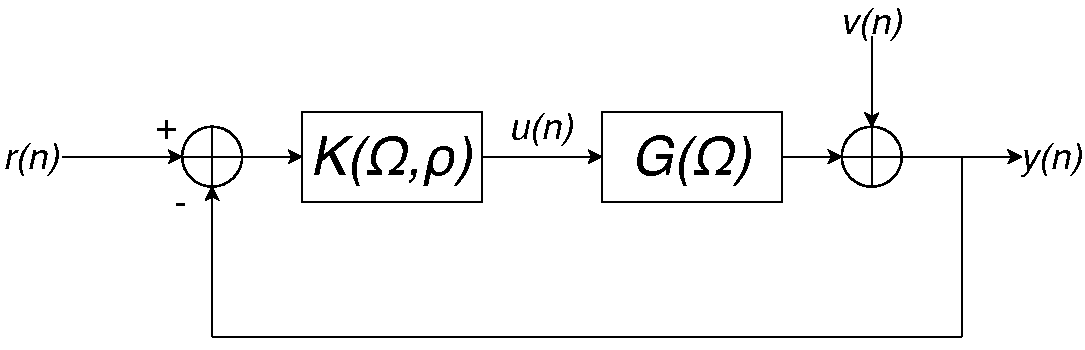
\includegraphics[width = 0.65\textwidth]{figures/closed_loop_system.pdf}
    \caption{Closed loop system.}
    \label{fig:closed_loop_system}
\end{figure}

The transfer function from the reference $r$ to the output $y$ is given by
\begin{equation*}
    \text{CL}(\Omega) = \frac{K(\Omega,\rho) G(\Omega)}{1 + K(\Omega,\rho) G(\Omega)}
\end{equation*}
$\rho = \begin{bmatrix}
        \rho_1 & \ldots & \rho_{n_{\rho}}
\end{bmatrix}^T$ is a vector containing the controller parameters that should be optimized. In this work $K(\Omega,\rho)$ is linear in the parameters.
\begin{equation}
    K(\Omega,\rho) = \beta(\Omega) \rho
    \label{eq:linear_in_the_parameters}
\end{equation}
with $\beta(\Omega)$ being a row vector with $n_\rho$ elements.
The idea of model reference control, is to get the closed loop system ``as close'' as possible to a user-defined reference system $M(\Omega)$.
\begin{equation*}
    \frac{K(\Omega,\rho) G(\Omega)}{1 + K(\Omega,\rho) G(\Omega)} \approx M(\Omega)
\end{equation*}
$M(\Omega)$ needs to be chosen such that it is a stable causal LTI system. Moreover, $M(\Omega)$ may not be chosen equal to 1. The reason for this is explained further on. This ``closeness'' criterion can be quantified by using the 2-norm of a transfer function.
\begin{equation}
    J_{mr}(\rho) =  \Big|\Big|F(\Omega) \Big[M(\Omega)-\frac{K(\Omega,\rho) G(\Omega)}{1 + K(\Omega,\rho) G(\Omega)}\Big]  \Big|\Big|_2^2 
    \label{eq:Jmr}
\end{equation}
$F(\Omega)$ is a user-defined weighing filter that can be chosen to highlight specific frequencies. The 2-norm of a SISO system is defined differently for CT and DT systems. For CT systems it is
\begin{equation*}
    ||H(s)||_2^2 = \frac{1}{2\pi} \int_{-\infty}^{+\infty} |H(j\omega)|^2 d\omega
\end{equation*}
and for DT systems it is
\begin{equation*}
    ||H(z^{-1})||_2^2 = \frac{1}{2\pi} \int_{-\pi}^{\pi} |H(e^{j\omega})|^2 d\omega
\end{equation*}

 \section{Convex cost}
A key problem with the use of (\ref{eq:Jmr}) as a cost function is that it is not convex.
In order to solve this, we must first define the ideal controller $K^*(\Omega)$ as
\begin{equation}
    K^*(\Omega) = \frac{M(\Omega)}{G(\Omega)(1-M(\Omega))}
    \label{eq:Kstar_def}
\end{equation}
This definition ensures that the closed loop system is equal to the reference system by construction.
\begin{equation*}
    \frac{K^*(\Omega) G(\Omega)}{1 + K^*(\Omega) G(\Omega)} = M(\Omega)
\end{equation*}
Note that it is possible that $K^*$ is not realizable i.e. 
\begin{equation*}
    \nexists \rho \text{ such that } K(\Omega,\rho) = K^*(\Omega)
\end{equation*}
For example, if $K^*(\Omega)$ is a polynomial of $\Omega$ of degree 4, then $K(\Omega,\rho) = \rho_0 + \rho_1\Omega + \rho_2\Omega^2$ will not be able to realize $K^*(\Omega)$ perfectly.

Next, both terms in (\ref{eq:Jmr}) can be put on the same denominator.
\begin{equation*}
    M(\Omega)-\frac{K(\Omega,\rho) G(\Omega)}{1 + K(\Omega,\rho) G(\Omega)} = \frac{M(\Omega)-(1-M(\Omega))K(\Omega,\rho) G(\Omega)}{1 + K(\Omega,\rho) G(\Omega)}
\end{equation*}
The sensitivity function is approximated by the ideal sensitivity function.
\begin{equation}
    \frac{1}{1 + K(\Omega,\rho) G(\Omega)} \approx \frac{1}{1 + K^*(\Omega) G(\Omega)} = \frac{1}{1+\frac{M(\Omega)}{1-M(\Omega)}} = 1-M(\Omega)
    \label{eq:approximation}
\end{equation}
The validity of this approximation should be verified afterwards. The sensitivity function is the transfer function from the disturbance $v(n)$ to the output $y(n)$. It quantifies how sensitive the output is to disturbances.

This approximation leads to the definition of the convex cost function.
\begin{equation}
\boxed{
    J(\rho) =  \Big|\Big|F(\Omega)(1-M(\Omega)) \Big[M(\Omega)-(1-M(\Omega))K(\Omega,\rho) G(\Omega)\Big]  \Big|\Big|_2^2 
    \label{eq:J}
}
\end{equation}
Of course, not all forms of $K(\Omega,\rho)$ will make this cost function convex. However, it is convex when $K(\Omega,\rho)$ is linear in the parameters (\ref{eq:linear_in_the_parameters}). Note that the cost is minimized for the ideal controller if the ideal controller is realizable.
\begin{equation*}
    K(\rho^*,\Omega) = K^*(\Omega) \Longrightarrow J(\rho^*) = 0
\end{equation*}
Note that (\ref{eq:J}) contains the factor $1-M(\Omega)$ as result of the approximation (\ref{eq:approximation}). If $M(\Omega)$ is chosen as 1, (\ref{eq:J}) would be equal to 0, which is the reason why $M(\Omega) = 1$ may not be used.
\section{Other cost functions}
We can devise many other cost functions that solve this problem. An example is the following.
\begin{equation}
    J_K(\rho) = ||K^*(\Omega)-K(\Omega,\rho)||_2^2
    \label{eq:JK}
\end{equation}
This cost function minimizes the square of the difference between the actual controller $K(\Omega,\rho)$ and the ideal controller $K^*(\Omega)$. If $K(\Omega,\rho)$ is linear in the parameters, then this is just a simple linear least squares regression. However, this is not the same as optimizing $\rho$ to the cost function (\ref{eq:J}) and will result in a different outcome. In fact, it can be shown that (\ref{eq:J}) is a weighted linear least squares regression version of (\ref{eq:JK}). By using (\ref{eq:Kstar_def}) we get
\begin{equation*}
    M(\Omega) = G(\Omega) (1-M(\Omega)) K^*(\Omega)
\end{equation*}
Using this expression in (\ref{eq:J}) results in
\begin{align*}
    J(\rho) & =  \Big|\Big|F(\Omega)(1-M(\Omega)) \Big[G(\Omega) (1-M(\Omega)) K^*(\Omega)-(1-M(\Omega))K(\Omega,\rho) G(\Omega)\Big]  \Big|\Big|_2^2 \\
    &= \Big|\Big|F(\Omega)(1-M(\Omega))^2 G(\Omega) \Big[ K^*(\Omega)-K(\Omega,\rho) \Big]  \Big|\Big|_2^2 
\end{align*}
Note that that $J(\rho)$ depends on $G(\Omega)$ both directly and indirectly as $K^*$ also depends on $G(\Omega)$. No expression for $G(\Omega)$ is known in the data-driven approach and it will therefore have to be estimated.
This shows that the choice of the cost function is an important part of the optimization and must be done with care.

\section{Correlation-based approach}
\label{sec:corr_based_approach}
As $G(\Omega)$ is not known in (\ref{eq:J}), the authors of \cite{Data-driven_model_reference_control} propose the correlation-based approach. They give algorithms for periodic and arbitrary excitations. Here we will focus on their equations concerning periodic excitations. We will also restrict this section to DT systems ($\Omega = z^{-1}$), as they have done in their paper.

One thing to note, is that all the equations in \cite{Data-driven_model_reference_control} are written in the TD. These will be translated to the FD in section \ref{sec:freq_domain_translate}. The reader is recommended to not spend too much time trying to understand the definitions in this section as they will make more sense in the next section.

\paragraph{Model}
First it is assumed that the output of the DT system is perturbed by some noise $v(n)$.
\begin{equation}
    y(n) = G(q^{-1}) u(n) + v(n)
    \label{eq:model_TD}
\end{equation}
with $q^{-1}$ being the backshift operator: $q^{-1} x(n) = x(n-1)$. $N$ denotes the period of the input.
\begin{equation}
    u(n) = u(n+N)
    \label{eq:periodicity_u}
\end{equation}
The additive noise is modelled as DT filtered white noise.
\begin{equation*}
    v(n) = S_v(q^{-1}) e_v(n) \,, \text{ with } \mathbb{E}\{e_v(n)\} = 0 \text{ and } \mathbb{E}\{e_v(n)^2\} = \sigma^2
\end{equation*}

\paragraph{Error signal}
Then a new quantity $\epsilon(n,\rho)$ is defined \cite[eq. (15)]{Data-driven_model_reference_control}.
\begin{align*}
    \epsilon(n,\rho) &= M(q^{-1}) u(n) - K(q^{-1},\rho) (1-M(q^{-1})) y(n) & \text{(computational form)} \\
    &= [M-K(\rho) (1-M) G ] u(n) - K(\rho) (1-M) v(n) & \text{(analytic form)} 
\end{align*}
In the second equality the operators $q^{-1}$ are left out for clarity. The computational form is used in practice because measurements $u(n)$ and $y(n)$ are available. The analytic form is used to develop the theory further.

Notice that when $K(\rho) = K^*$, the first term in the analytic form is zero.
\begin{equation*}
	\epsilon^*(n) = -K^*(1-M)v(n)
\end{equation*}
Thus $\epsilon(n,\rho)$ is uncorrelated with $u(n)$ when $\rho = \rho^*$. The main idea behind the correlation-based approach is to tune the parameters $\rho$ such that $\epsilon(n,\rho)$ becomes uncorrelated with $u(n)$. However, note that this reasoning only holds if $K^*$ is realizable with the proposed controller scheme $K(\rho)$. If $K^*$ is not realizable, then the first term $[M-K(\rho) (1-M) G ]$ will not be zero when replacing $K(\rho)$ with the ideal controller $K^*$ and $\epsilon(n,\rho)$ will still be correlated with $u(n)$.


\paragraph{Input filtering}
Additionally, the filter $W$ is defined \cite[eq. (41)]{Data-driven_model_reference_control}
\begin{align*}
    W(e^{-j\omega_k}) &= \frac{F(e^{-j\omega_k})(1-M(e^{-j\omega_k}))}{S_{UU}(e^{-j \omega_k})} \\
    \omega_k &= \frac{2\pi k}{N} \,,\quad k=0,\ldots,N-1
\end{align*}
$S_{UU}(e^{-j \omega_k})$ is the DFT of the autocorrelation of $u(n)$ \cite[eqs. (38) and (39)]{Data-driven_model_reference_control}.
\begin{align}
    R_{uu}(\tau) &= \frac{1}{N}\sum_{n=0}^{N-1} u(n-\tau) u(n) \label{eq:Rutau}\\
    S_{UU}(e^{-j \omega_k}) &=  \sum_{\tau=0}^{N-1} R_{uu}(\tau) e^{-j \tau \omega_k}\label{eq:Suu}
\end{align}
If the system is in steady state, $u(n-\tau)$ is known for negative time indices by using (\ref{eq:periodicity_u}). If the experiment starts with zero initial conditions, then $u(n-\tau) = 0$ for $n-\tau < 0$.

The filter $W$ is applied to the input $u(n)$. As is remarked at the end of \cite[Sec. 4.4]{Data-driven_model_reference_control}, if a parametric representation of $S_{UU}(q^{-1})$ is known, this filter can be applied in the TD.
\begin{equation*}
    u_W(n) = W(q^{-1}) u(n)
\end{equation*}
Note that this can be problematic if $S_{UU}(q^{-1})$ has zeros that are not on the unit circle, as the filter $W(q^{-1})$ will then be unstable. More information concerning this is given in appendix \ref{appendix:W_filtering}.

\paragraph{Correlation criterion}
Then, the cross-correlation between between $u_W(n)$ and $\epsilon(n,\rho)$ is calculated.
\begin{equation}
    R_{u_W \epsilon}(\tau,\rho) = \frac{1}{N\!P} \sum_{n=0}^{N\!P-1} u_W(n-\tau) \epsilon(n,\rho)
    \label{eq:RuWepstau}
\end{equation}
with $P$ being the number of periods measured. Note that as in (\ref{eq:Rutau}), $u_W(n-\tau)$ can be found by using (\ref{eq:periodicity_u}) if the system is in steady state. If the system starts off in zero initial conditions, $u_W(n-\tau) = 0$ for $n-\tau < 0$.

The correlation criterion $J_{N\!P,l_1}(\rho)$ can then be defined.
\begin{equation}
\boxed{
    J_{N\!P,l_1}(\rho) = \sum_{\tau=-l_1}^{l_1} R_{u_W \epsilon}^2(\tau,\rho)
}
\label{eq:JNl1}
\end{equation}
with $l_1 \leq N/2$ being a parameter that can be chosen by the user. The idea behind this parameter $l_1$ is discussed in detail in section \ref{sec:parseval}. It is then proven in \cite[Appendix II]{Data-driven_model_reference_control} that (\ref{eq:JNl1}) converges to (\ref{eq:J}) for $N,P \rightarrow \infty$ with probability 1 under certain conditions.
\begin{equation*}
    \lim_{N,P\rightarrow \infty} J_{N\!P,l_1}(\rho) = J(\rho) \,,\, \text{w.p. } 1
\end{equation*}
However, for finite data, it is proven that the estimator is biased \cite[eq. (37)]{Data-driven_model_reference_control}. The bias is discussed further in section \ref{sec:bias}.

\section{Translation to the frequency domain}
\label{sec:freq_domain_translate}
In this section the results from the previous section will be translated to the FD. Here we will show that a nonparametric estimate of the system $G(\Omega)$ is actually hidden in the mathematics. Thus, even though the parametric modelling step is skipped, there is still a nonparametric model.

\subsection{Disadvantages of TD}
There are some disadvantages of working in the TD. Here are some that are relevant to this subject.
\begin{itemize}
    \item TD filtering can only be done easily if the underlying system is a DT system.
    \item The filtering of $u(n)$ with $W(q^{-1})$ can only be performed in the TD if a parametric representation of $S_{UU}(q^{-1})$ is known and if $S_{UU}(q^{-1})$ only has zeros on the unit circle. (see appendix \ref{appendix:W_filtering}).
    \item If the system starts with zero initial conditions or in steady state, then the transient response can be taken into account, as knowledge of the input and output signals are known before they are applied. This makes it possible to calculate (\ref{eq:Rutau}) and (\ref{eq:RuWepstau}) for $n-\tau < 0$. However, if the system does not start with zero initial conditions or in steady state, this approach will not work and the transient term will not be suppressed.
\end{itemize}
These problems can be solved by working in the FD. To address the first point: FD methods can also handle CT systems. For the second point: a convolution in the TD will explode when the system is unstable. However, this is not a problem in the FD as a convolution in the TD becomes a simple multiplication in the FD. Finally, for the third point: the robust LPM (see section \ref{sec:LPM}) is able to estimate nonparametrically the frequency response function (FRF) from noisy input-output data, while suppressing the transient term.


% For the remainder of this section, a simplified approach to estimating the FRF is used to illustrate how the TD algorithm outlined in the beginning of this section can be translated to the FD.

% First, the DFT of the input u(n) and output y(n) is defined. As before, I assume that $u(n)$ is periodic with a period of $N$ samples. $n_p$ periods of $y(n)$ are measured.

% \begin{align*}
%     U^{(m)}(k) &= \text{DFT}\{ u^{(m)}(n) \}(k) \,,\, k = 0,\ldots,N-1\\
%     Y^{(m)}(k) &= \text{DFT}\{ y^{(m)}(n) \}(k)  \,,\, k = 0,\ldots,N-1
% \end{align*}
% with the superscript $(m)$ denoting the period ($m = 1,\ldots,n_p$). Working with periodic data allows for taking the mean of the spectra over the DFT bins.
% \begin{align*}
%     U(k) &= \frac{1}{P} \sum_{m=1}^{P} U^{(m)}(k) \\
%     Y(k) &= \frac{1}{P} \sum_{m=1}^{P} Y^{(m)}(k)
% \end{align*}
% The auto power spectrum of $u(n)$ is simply 
% \begin{equation*}
%     S_{UU}(\Omega_k) = U(k) \overline{U(k)}
% \end{equation*}
% with $\overline{\bullet}$ denoting the complex conjugate operator. FD methods are not restricted to DT systems. So $\Omega_k$ is defined as:

% \begin{equation*}
%     \Omega_k = \begin{cases}
%         j 2 \pi k F_s/N & \text{if working in continuous-time (CT)} \\
%         e^{j 2 \pi k/N}& \text{if working in discrete-time (DT)} 
%     \end{cases}
% \end{equation*}
% $F_s$ is the sampling frequency.
\subsection{Nonparametric estimate}
By translating the formulas of section \ref{sec:corr_based_approach} to the FD, it will become immediately apparent that a nonparametric estimate of the FRF is being calculated. The first step in translating the problem from the TD to the FD is to use Parseval's theorem. According to Parseval's theorem, the sum of squares in the TD is equivalent to the sum of the norms squared in the FD. The cost function (\ref{eq:JNl1}) represents a sum of squares in the TD. Parseval's theorem will be discussed in greater detail in section \ref{sec:parseval}.

Now, instead of calculating $\epsilon(n,\rho)$ in the TD, it can be calculated in the FD. Note that this also makes the computations less intensive, as a convolution in the TD becomes a multiplication in the FD. As the input to the system is assumed to be periodic  with period $P$, the frequencies $\Omega_k$ will correspond to the DFT bins $kP$.
\begin{equation*}
    E(kP,\rho) = M(\Omega_k) U(kP) - K(\Omega_k,\rho) (1-M(\Omega_k)) Y(kP)
\end{equation*}
Applying the filter $W$ to $u(n)$ can also be done in the FD.
\begin{equation*}
    U_W(kP) = W(\Omega_k) U(kP)
\end{equation*}
with
\begin{equation*}
    W(\Omega_k) = \frac{F(\Omega_k)(1-M(\Omega_k))}{S_{UU}(e^{-j \omega_k})}
\end{equation*}
The denominator $S_{UU}(e^{-j \omega_k})$ is proportional to $U(kP)\overline{U(kP)}$.
\begin{equation}
S_{UU}(e^{-j \omega_k}) = N U(kP)\overline{U(kP)}
\label{eq:Suu=NUU}
\end{equation}
This equivalence is proven in appendix \ref{appendix:DFT_cross}. Then, the cross-power spectrum between $\epsilon(n,\rho)$ and $u_W(n)$ is also calculated in the FD by doing a simple multiplication.
\begin{equation}
    S_{U_W\!E}(\Omega_k,\rho) = N U_W(kP) \overline{E(kP,\rho)}
    \label{eq:RWE_FD}
\end{equation}
Expanding (\ref{eq:RWE_FD}) makes the link to the cost function (\ref{eq:J}) immediately apparent.
\begin{align}
    S_{U_W\!E}(\Omega_k,\rho) &= U(kP) \frac{F(1-M)}{U(kP)\overline{U(kP)}}  \overline{ \big(M U(kP) - K(\rho) (1-M) Y(kP) \big)} \label{eq:PhiUwepsilon_FD}\\
    &= F (1-M) \overline{\big( M - K(\rho) (1-M)\hat{G}(\Omega_k) \big)}
    \label{eq:cross-power_in_FD}
\end{align}
with 
\begin{equation}
    \hat{G}(\Omega_k) = \frac{Y(kP) \overline{U(kP)}}{U(kP) \overline{U(kP)}} = \frac{Y(kP)}{U(kP)}
    \label{eq:Ghat=YU/UU}
\end{equation}
The index $\Omega_k$ was left out in $F$, $M$ and $K$ for clarity.
$\hat{G}(\Omega_k)$ is a nonparametric estimate of the system. If $\hat{G}$ is replaced by the actual system $G$, then $S_{U_W\!E}(\Omega_k,\rho)$ is exactly the quantity being integrated over in (\ref{eq:J}).

\newpage
Thus, a nonparametric estimate of the system $\hat{G}$ can be found, followed by calculating the cost function in the FD.
\begin{equation}
\boxed{
    J_N(\rho) = \frac{1}{|\kexc|}\sum_{k \in \kexc} \Big|H(\Omega_k,\rho)\Big|^2
\label{eq:JFD}
}
\end{equation} 
with $\kexc$ being the set of excited DFT bins, $|\kexc|$ being the cardinality of this set and
\begin{equation}
    H(\Omega_k,\rho) = F(\Omega_k)(1-M(\Omega_k)) \Big[M(\Omega_k)-(1-M(\Omega_k))K(\Omega_k,\rho) \hat{G}(\Omega_k)\Big]
\end{equation}
Proceeding in this way, we can be much more flexible with the manner in which we estimate the FRF nonparametrically. Let's take a closer look at the nonparametric estimator that is hidden inside the formulas of the TD.
\begin{equation*}
    \hat G(\Omega_k) = \frac{Y(kP)}{U(kP)}
\end{equation*}
Now, let's separate $y(n)$ into its $P$ periods $y^{(p)}(n)$.
\begin{equation*}
    y^{(p)}(n) = y(n+pP) \,,\quad p = 0,\ldots,P-1
\end{equation*}
We can also define the DFT for each of the periods.
\begin{equation*}
    Y^{(p)}(k) = \frac{1}{N}\sum_{n=0}^{N-1} y^{(p)}(n) e^{-j2\pi kn/N} \,,\quad p = 0,\ldots,P-1
\end{equation*}
With these definitions we can get a better understanding of what $Y(kP)$ represents.
\begin{align*}
    Y(kP) &= \frac{1}{N P}\sum_{n=0}^{N\!P-1} y(n) e^{-j2\pi (kP) n/(N\!P)}\\
    &= \frac{1}{N P} \sum_{p=0}^{P-1}  \sum_{n=0}^{N-1} y(n+pP) e^{-j2\pi kn/N} = \frac{1}{P} \sum_{p=0}^{P-1} Y^{(p)}(k)
\end{align*}
Thus, the nonparametric estimate becomes
\begin{equation}
    \hat G(\Omega_k) = \frac{\frac{1}{P}\sum_{p=0}^{P-1}  Y^{(p)}(k)}{\frac{1}{P}\sum_{p=0}^{P-1}  U^{(p)}(k)}
    \label{eq:nonparametric_simple}
\end{equation}
This is a consistent estimator for the model (\ref{eq:model_TD}). Indeed, if we translate (\ref{eq:model_TD}) to the FD we obtain
\begin{equation*}
    Y^{(p)}(k) = G(\Omega_k) U^{(p)}(k) + V^{(p)}(k) \,,\quad p = 0,\ldots,P-1
\end{equation*}
Given that the input is periodic $U^{(p)}(k) = U_0(k)$, we get
\begin{equation*}
    \hat G(\Omega_k) = \frac{\frac{1}{P}\sum_{p=0}^{P-1} \Big [ G(\Omega_k) U_0(k) + V^{(p)}(k) \Big ]}{U_0(k)} = G(\Omega_k) + \frac{1}{U_0(k)} \frac{1}{P}\sum_{p=0}^{P-1} V^{(p)}(k)
\end{equation*}
The output noise is assumed to be Gaussian white noise, which means that $\mathbb{E}\{V(k)\}=0$. Taking the limit for $P \rightarrow \infty$ gives
\begin{equation*}
    \lim_{P \rightarrow \infty} \hat G(\Omega_k) = G(\Omega_k) + \frac{1}{U_0(k)} \mathbb{E}\{V(k)\} = G(\Omega_k) \,,\, \text{w.p. } 1
\end{equation*}
The law of large numbers for independent experiments is used in the first equation. Following the same lines, it can easily be verified that the estimator is also consistent if the measurement of the input is noisy.
\begin{equation*}
    U^{(p)} = U_0(k) + N_U^{(p)}(k)
\end{equation*}

\newpage
\section{Parseval's theorem}
\label{sec:parseval}
Parseval's theorem is very simple: the energy of the signal in the TD is the same as the energy of the signal in the FD.
\begin{equation}
    \sum_{n=0}^{N-1} x(n)^2 = N \sum_{k=0}^{N-1} |X(k)|^2
    \label{eq:parseval_theorem}
\end{equation}
with $X(k) = \text{DFT}\{x(n)\}$. The factor $N$ is specific to the definition of the DFT that is used in this work and will be different if another definition is used.

The cost function in the FD (\ref{eq:JFD}) is also the sum of squares.
\begin{equation*}
    J_N(\rho) = \frac{1}{N} \sum_{k=0}^{N-1} |H(\Omega_k,\rho)|^2
\end{equation*}
According to Parseval's theorem, the above sum is equivalent to a sum of squares in the TD.
\begin{equation}
    J_N(\rho) = \frac{1}{N^2}\sum_{n=0}^{N-1} h(n,\rho)^2
    \label{eq:JN_TD}
\end{equation}
with $h(n,\rho)$ being the IDFT of $H(\Omega_k,\rho)$. If $N \rightarrow \infty$, $h(n,\rho)$ is the impulse response of the system $H(\Omega,\rho)$. The trick that the authors use in \cite{Data-driven_model_reference_control} is the fact that the impulse response of a stable system will fade away after some time.
\begin{equation*}
    \exists l_1 \text{ such that } h(n) \approx 0 \text{ for } n > l_1
\end{equation*}
Applying this approximation to the cost function (\ref{eq:JN_TD}), gives
\begin{equation}
    J_N(\rho) \approx  \frac{1}{N^2} \sum_{n=0}^{l_1} h(n,\rho)^2
    \label{eq:Japprox_impulse_response}
\end{equation}


\paragraph{Example}
Let's take a very simple first order system.
\begin{equation}
    H(z^{-1}) = \frac{0.2 z^{-1}}{1 - 0.8 z^{-1}}
    \label{eq:parseval_example_H}
\end{equation}
The first 51 samples of the impulse response of (\ref{eq:parseval_example_H}) are plotted in figure \ref{fig:parseval_signal}. Additionally, the red dotted line shows the impulse response with a bit of additive Gaussian white noise.

\begin{figure}[H]
    \centering
    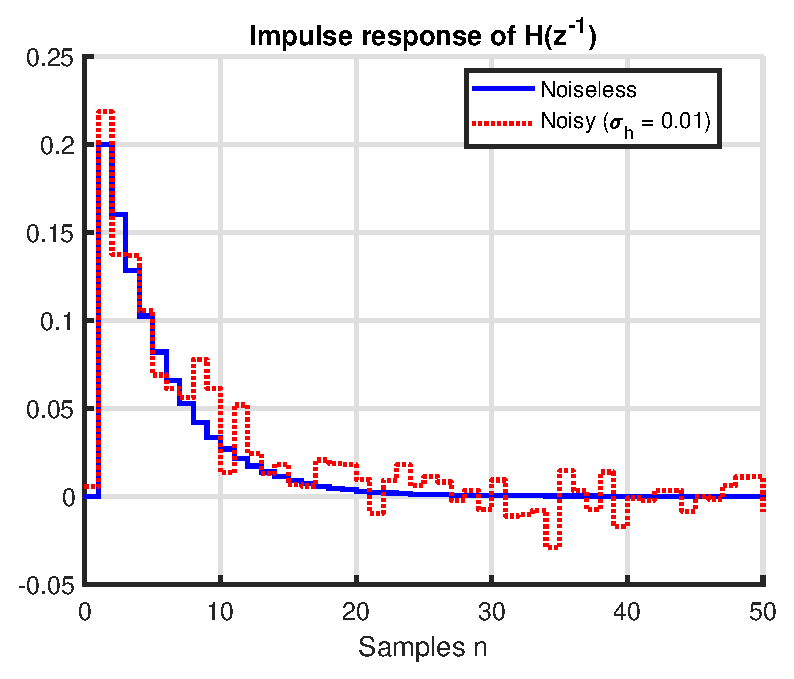
\includegraphics[width = 0.65 \textwidth]{figures/parseval_signal.eps}
    \caption{Impulse response of (\ref{eq:parseval_example_H}) with and without additive Gaussian white noise.}
    \label{fig:parseval_signal}
\end{figure}

The approximate cost function of the signal in the TD $\frac{1}{51^2}\sum_{n=0}^{l_1} h(n,\rho)^2$ is plotted in figure \ref{fig:parseval_energy} (blue full line). It quickly converges to the cost function of the signal in the FD $\frac{1}{51} \sum_{k=0}^{50} |H(k)|^2$. This is also the case for the noisy signal (dotted red line); it converges to its cost in the FD. Ideally however, we would like the cost in the noisy case to be as close to the actual, noiseless cost. This is not the case; there is a certain bias. In this case, taking $l_1 = 10$, would result in less bias, while still keeping the information that is needed. This can also be seen in figure \ref{fig:parseval_signal}: the impulse response after $n = 10$ is at or below noise level. Thus the impulse response after $n = 10$ does not contain much useful information and will only contribute to a biased cost.

\begin{figure}[H]
    \centering
    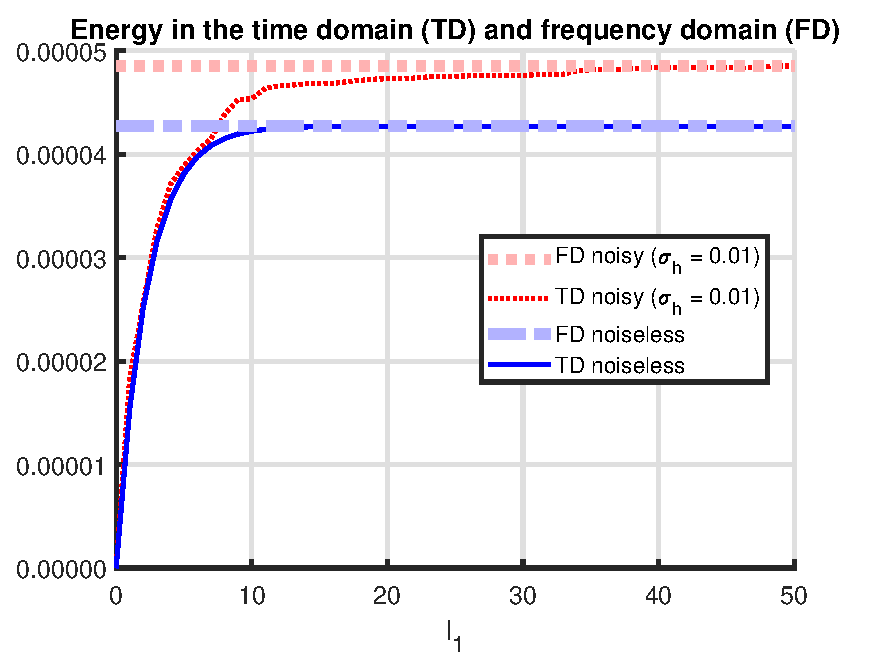
\includegraphics[width = 0.65 \textwidth]{figures/parseval_energy.eps}
    \caption{Energy of the signal in the TD and the FD (divided by $N$).}
    \label{fig:parseval_energy}
\end{figure}

In \cite{Data-driven_model_reference_control}, $l_1$ has a slightly different interpretation. As it can be seen in (\ref{eq:JNl1}), the sum goes from $-l_1$ to $l_1$. This is because the sum is taken over the cross-correlation of $u_W$ and $\epsilon$. The cross-correlation is meaningful for both positive and negative indices, which is why the sum also extends into negative values of $\tau$. The impulse response for negative indices is zero for causal systems, which is why the sum starts at $n = 0$ in (\ref{eq:Japprox_impulse_response}).

\newpage
\section{Bias}
\label{sec:bias}
Let's quantify the bias that was mentioned in the previous section. Let's assume that the input is a periodic signal that excites all the DFT frequencies. The output is perturbed by filtered white noise.
\begin{equation*}
    Y^{(p)}(k) = G(\Omega_k)U_0(k) + S_v(\Omega_k) V^{(p)}(k)
\end{equation*}
with $\mathbb{E}\{V^{(p)}(k)\} = 0$ and $\mathbb{E}\{|V^{(p)}(k)|^2\} = \sigma^2/N$. The nonparametric estimate of the FRF is
\begin{equation*}
    \hat G(\Omega_k) = \frac{\frac{1}{P}\sum_{p=0}^{P-1}  Y^{(p)}(k)}{\frac{1}{P}\sum_{p=0}^{P-1}  U^{(p)}(k)} = G(\Omega_k) + \frac{1}{U_0(k)} \frac{1}{P}\sum_{p=0}^{P-1} S_v(\Omega_k) V^{(p)}(k)
\end{equation*}
The statistical properties of this estimator are
\begin{align*}
    \mathbb{E}\{\hat G(\Omega_k)\} &= G(\Omega_k)\\
    \mathrm{Var}\{|\hat G(\Omega_k)|\} &= \frac{1}{N\!P}\frac{|S_v(\Omega_k)|^2 \sigma^2}{|U_0(k)|^2}
\end{align*}
$|S_v(\Omega_k)|^2 \sigma^2$ quantifies the power of the noise at the $k$-th DFT bin and $|U_0(k)|^2$ quantifies the energy of the signal at the $k$-th bin. This becomes evident when the RMS of the signals is calculated.
\begin{equation*}
    \text{RMS} = \sqrt{\frac{1}{N}\sum_{n=0}^{N-1} x(n)^2} = \sqrt{\sum_{k=0}^{N-1} |X(k)|^2}
\end{equation*}
Thus, $\frac{|S_v(\Omega_k)|^2 \sigma^2}{|U_0(k)|^2}$ is the noise-to-signal ratio at the $k$-th DFT bin.

Now we have the information we need to calculate the expected value of the cost function.
\begin{equation*}
    J_N(\rho) = \frac{1}{N}\sum_{k=0}^{N-1} |H(\Omega_k,\rho)|^2 = \frac{1}{N} \sum_{k=0}^{N-1} \Bigg|F(\Omega_k)(1-M(\Omega_k)) \Big[M(\Omega_k)-(1-M(\Omega_k))K(\Omega_k,\rho) \hat{G}(\Omega_k)\Big]\Bigg|^2
\end{equation*}
Taking the expected value gives
\begin{align*}
    \mathbb{E}\{J_N(\rho)\} &= \frac{1}{N}\sum_{k=0}^{N-1} \Bigg|F(\Omega_k)(1-M(\Omega_k)) \Big[M(\Omega_k)-(1-M(\Omega_k))K(\Omega_k,\rho) G(\Omega_k)\Big]\Bigg|^2 \\
    &+ \frac{1}{N} \sum_{k=0}^{N-1} \frac{1}{N\!P} \frac{|S_v(\Omega_k)|^2 \sigma^2}{|U_0(k)|^2} \Bigg|F(\Omega_k)(1-M(\Omega_k))^2 K(\Omega_k,\rho) \Bigg|^2  \\
    &= \Tilde{J}_N(\rho) + \frac{\sigma^2}{N^2 P} \sum_{k=0}^{N-1} \frac{|F(\Omega_k)|^2|1-M(\Omega_k)|^4 |K(\Omega_k,\rho)|^2}{\text{SNR}(k)}
\end{align*}
with $\Tilde{J}_N(\rho)$ being the cost function in the noiseless case and $\text{SNR}(k) = \frac{|U_0(k)|^2}{|S_v(\Omega_k)|^2 \sigma^2}$. So, it has been shown that the expected value of the cost function in the noisy case is not equal to the noiseless cost function. This is not a problem if the second term does not depend on $\rho$, as the optimization parameters that minimize $\mathbb{E}\{J_N(\rho)\}$ would also minimize $\Tilde{J}_N(\rho)$. However, in this case the second term does depend on $\rho$, which is the cause of the noise induced bias.

What if we now transform $H(\Omega_k,\rho)$ to the TD using the IDFT and approximate the cost function by only summing till $l_1$?
\begin{equation*}
    J_N(\rho) = \frac{1}{N} \sum_{k=0}^{N-1} |H(\Omega_k,\rho)|^2 = \frac{1}{N^2}\sum_{n=0}^{N-1} h(n,\rho)^2 \approx  \frac{1}{N^2}\sum_{n=0}^{l_1} h(n,\rho)^2 = J_{N,l_1}(\rho)
\end{equation*}
Because the sum only contains $(l_1+1)$ noisy terms, the bias will be smaller compared with the full sum. To be more specific, the bias will be a factor $(l_1+1)/N$ smaller. Thus the expected value of the approximate cost function becomes
\begin{equation}
\boxed{
    \mathbb{E}\{J_{N,l_1}(\rho)\} \approx \Tilde{J}_N(\rho) +  \frac{\sigma^2}{N^2 P} \frac{l_1+1}{N} \sum_{k=0}^{N-1} \frac{|F(\Omega_k)|^2|1-M(\Omega_k)|^4 |K(\Omega_k,\rho)|^2}{\text{SNR}(k)}
    }
    \label{eq:EJl1_FD}
\end{equation}
Thus, the bias can be decreased by only taking the first $l_1+1$  terms in the TD. However, making $l_1$ too small will invalidate the approximation $J_N(\rho) \approx J_{N,l_1}(\rho)$. Additionally, the bias can also be decreased by increasing the number of periods $P$, increasing the number of samples per period $N$ or by increasing the signal-to-noise ratio $\textrm{SNR}(k)$.

\section{Weighted nonlinear least squares}
\label{sec:WNLS}
It is possible to reduce the variability by using a weighted cost function. The weights will be based on the variance of the FRF estimate.
\begin{align*}
    \sigma^2_{\hat G}(\Omega_k) = \mathbb{E}\big\{|\hat G(\Omega_k)- \mathbb{E}\{\hat G(\Omega_k)\}|^2\big\} 
\end{align*}
The robust LPM can estimate the variance of the FRF estimate $\hat\sigma^2_{\hat G}$ for systems excited by periodic inputs. The weighted nonlinear least squares cost function is
\begin{equation}
\boxed{
    J_\mathrm{WNLS}(\rho) = \frac{1}{|\kexc|}\sum_{k \in \kexc} \frac{|H(\Omega_k,\rho)|^2}{\hat\sigma^2_{H}(\Omega_k,\rho)}}
    \label{eq:JWNLS}
\end{equation}
with $\kexc$ being the set of excited DFT bins and
\begin{equation*}
    H(\Omega_k,\rho) = F(\Omega_k)(1-M(\Omega_k)) \Big[M(\Omega_k)-(1-M(\Omega_k))K(\Omega_k,\rho) \hat{G}(\Omega_k)\Big]
\end{equation*}
and
\begin{equation*}
\hat\sigma^2_{H}(\Omega_k,\rho) = \hat\sigma^2_{\hat G}(\Omega_k) \Big| F(\Omega_k) (1-M(\Omega_k))^2K(\Omega_k,\rho) \Big|^2
\end{equation*}


The expected value of (\ref{eq:JWNLS}) is
\begin{align*}
\mathbb{E}\{J_\mathrm{WNLS}(\rho)\} &=
 \frac{1}{|\kexc|} \sum_{k \in \kexc} \frac{|F(1-M)|^2 |M-(1-M)K(\rho)G|^2}{|F(1-M)^2 K(\rho)|^2 \hat\sigma^2_{\hat G}}\\ 
 &+ \frac{1}{|\kexc|} \sum_{k \in \kexc} \frac{|F(1-M)^2 K(\rho)|^2 \sigma^2_{\hat G}}{|F(1-M)^2 K(\rho)|^2 \hat\sigma^2_{\hat G}} \\
&=  \Tilde{J}_\mathrm{WNLS}(\rho) + \frac{1}{|\kexc|} \sum_{k \in \kexc} \frac{\sigma^2_{\hat G}(\Omega_k)}{\hat\sigma^2_{\hat G}(\Omega_k)} 
\end{align*}
with $\Tilde{J}_\mathrm{WNLS}(\rho)$ being the cost function when $G(\Omega_k)$ is known exactly. The frequencies $\Omega_k$ are left out in the first equation for simplicity. The second term does not depend on $\rho$, which means that the optimization parameters $\rho$ that minimize $\mathbb{E}\{J_\mathrm{WNLS}(\rho)\}$ will also minimize $\Tilde{J}_\mathrm{WNLS}(\rho)$. After all, the second term is just a constant independent of $\rho$.


\paragraph{Realizable ideal controller}
If the ideal controller is realizable, then
\begin{equation*}
\Tilde{J}_\mathrm{WNLS}(\rho^*) = 0
\end{equation*}
The convex cost function (\ref{eq:JFD}) is also zero in $\rho = \rho^*$ in the noiseless case. This means that the original cost function (\ref{eq:Jmr}), the convex cost function (\ref{eq:J}) and the WNLS cost function (\ref{eq:JWNLS}) are all minimal in $\rho = \rho^*$. Therefore, if the ideal controller is realizable, then the WNLS optimization has the potential to give a better estimate of the ideal controller as the WNLS cost function also takes the noise variance into account.


\paragraph{Non realizable ideal controller}
On the other, what happens if the ideal controller is not realizable? In this case, the minimum of any of the costs will be greater than 0, even in the noiseless case. Thus, the optimization parameters $\rho$ that minimize the original cost function, the convex cost function and the WNLS cost function will be different in general.


\paragraph{Optimization strategy}
The cost function (\ref{eq:JWNLS}) is not convex any more as the denominator also depends on the optimization parameters $\rho$. Thus, the minimization of this cost function cannot be solved with convex optimization. It can be solved with the Gauss-Newton algorithm. An initial estimate of $\rho$ can be found by minimizing the convex cost function (\ref{eq:JFD}). The danger however, is that this optimization might not converge to the global minimum.


\section{Summary}
The steps that must be taken in order to find a controller using model reference control are summarized in figure \ref{fig:flowchart}. Measurements of the (noisy) SISO system are given. These are necessary for the optimization.
%Note that the output is assumed to be perturbed by filtered white noise with noise model $S_y(q^{-1})$. However, the input can also be noisy and the different optimization strategies also work when this is the case. Moreover, no system is LTI in the real world. Nevertheless, it is still useful to assume that they are.

%Measurements of the system input and output are necessary for the optimization. 

The user must then also define the reference model $M(\Omega)$ and the controller structure $K(\Omega,\rho)$. Then, the user can choose one of the optimization criteria that were discussed in the previous sections. This results in the optimal parameters $\rho_{\mathrm{opt}}$, from which the optimal controller $K(\Omega,\rho_{\mathrm{opt}})$ can be determined.

\begin{figure}[H]
\centering
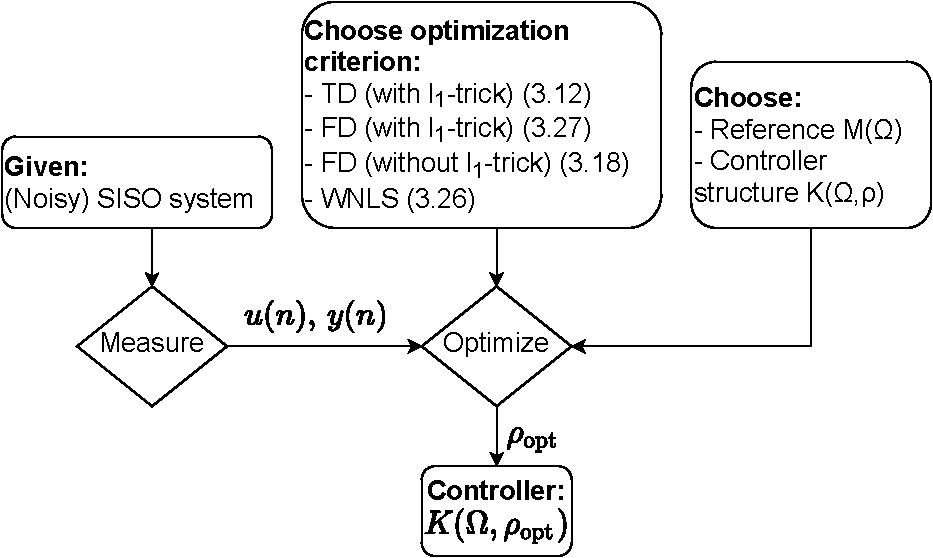
\includegraphics[width = 0.75\textwidth]{figures/flowchart.pdf}
\caption{Flowchart of the steps taken in model reference control.}
\label{fig:flowchart}
\end{figure}


\newpage
\section{Discrete-time simulations}
\label{sec:DT_simulations}

\subsection{Introduction}
\label{sec:DT_simulations_introduction}
First, an important approximation was made in the previous sections. Initially, it was assumed that the sensitivity function can be approximated by the ideal sensitivity function.
\begin{equation*}
\frac{1}{1 + K(\Omega,\rho) G(\Omega)} \approx \frac{1}{1 + K^{*}(\Omega) G(\Omega)}
\end{equation*}
This was done in order to make the cost function convex. Thus we should verify after optimization that the original cost function (\ref{eq:Jmr}) can be approximated by the convex cost function (\ref{eq:J}).
\begin{equation*}
	J_{mr}(\rho) \approx J(\rho)
\end{equation*}

\paragraph{System models}
In order to compare the FD methods to the TD methods, we will initially work with DT systems. 3 DT systems $G(q^{-1})$ will be simulated. The first 2 systems will have a reference model $M(q^{-1})$ that will be realizable by the proposed control structure $K(q^{-1},\rho)$. The third system will have a reference model that cannot be realized by the proposed control structure. The systems, the reference models and the proposed controller structures are given in table \ref{tab:simulated_systems}. These are also shown in figure \ref{fig:G_and_M_all}. The systems will start with zero initial conditions.

\begin{table}[H]
\centering
\begin{tabular}{|ccc|}
\hline
Name & Simple system & Long transient system\\
\hline
&&\\[-2.5ex]
$G(q^{-1})$ & $\dfrac{0.25 q^{-1}}{1 - 0.75 q^{-1}}$ & $\dfrac{1.785 q^{-1} + 1.701 q^{-2}}{1 + 1.558 q^{-1} + 0.9274 q^{-2}}$ \\
\hline
&&\\[-2.5ex]
$M(q^{-1})$ & $\dfrac{0.15 q^{-1} - 0.075 q^{-2}}{1 - 1.6 q^{-1} + 0.675 q^{-2}}$ & $\dfrac{0.1785 q^{-1} + 0.3486 q^{-2} + 0.1701 q^{-3}}{1 + 0.7369 q^{-1} - 0.2824 q^{-2} - 0.7573 q^{-3}}$ \\
\hline
&&\\[-2.5ex]
$K(\rho,q^{-1})$ & $\dfrac{\rho_0 + \rho_1 q^{-1}}{1-q^{-1}}$ & $\dfrac{\rho_0 + \rho_1 q^{-1}}{1-q^{-1}}$ \\
\hline
Realizable & Yes & Yes \\
\hline
\hline
Name & \multicolumn{2}{c|}{System with non realizable controller} \\
\hline
&&\\[-2.5ex]
$G(q^{-1})$ & \multicolumn{2}{c|}{$\dfrac{0.7893 q^{-3}}{1 - 1.418 q^{-1} + 1.59 q^{-2} - 1.316 q{^-3} + 0.886 q^{-4}}$}\\
\hline
&&\\[-2.5ex]
$M(q^{-1})$ & \multicolumn{2}{c|}{$\dfrac{0.1552 q^{-3}}{1 - 1.212 q^{-1} + 0.3672 q^{-2}}$} \\
\hline
&&\\[-2.5ex]
$K(\rho,q^{-1})$ & \multicolumn{2}{c|}{$\dfrac{\rho_0 + \rho_1 q^{-1} + \rho_2 q^{-2} + \rho_3 q^{-3} + \rho_4 q^{-4}}{1-q^{-1}}$} \\
\hline
Realizable & \multicolumn{2}{c|}{No} \\
\hline
\end{tabular}
\caption{Simulated system and the reference models.}
\label{tab:simulated_systems}
\end{table}


\begin{figure}[H]
\centering
\begin{subfigure}{.33\textwidth}
	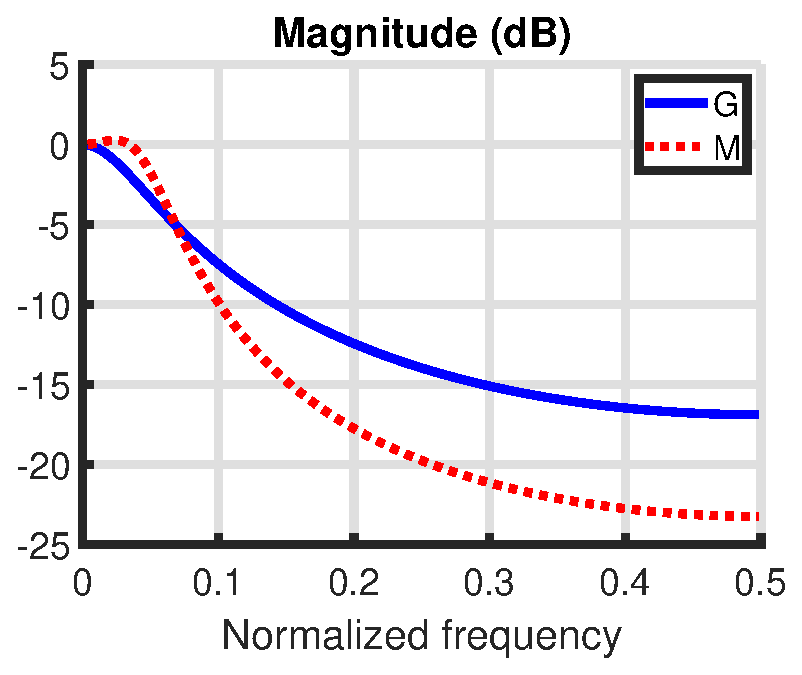
\includegraphics[width=\linewidth]{figures/G_and_M_simple.eps}
	\caption{Simple system}
\end{subfigure}%
\begin{subfigure}{.33\textwidth}
	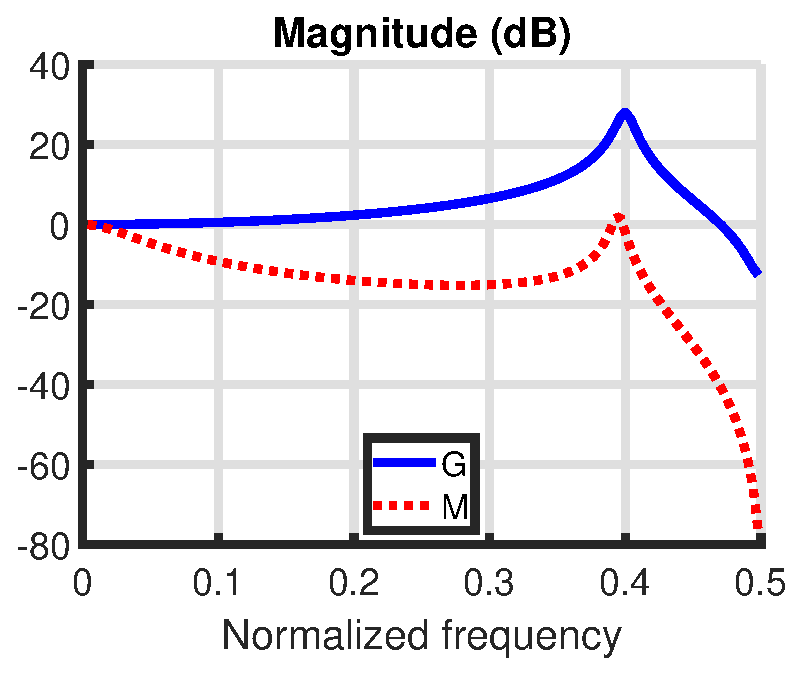
\includegraphics[width=\linewidth]{figures/G_and_M_long_transient.eps}
	\caption{Long transient system}
\end{subfigure}%
\begin{subfigure}{.33\textwidth}
	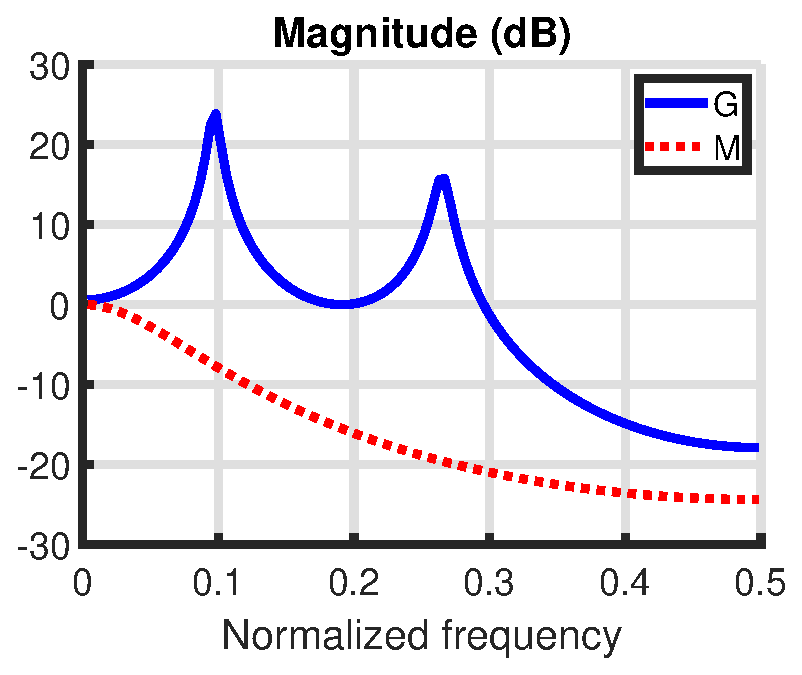
\includegraphics[width=\linewidth]{figures/G_and_M_undermodeled.eps}
	\caption{System with non realizable controller}
\end{subfigure}
\caption{Magnitude bode plots of the system and the reference models.}
\label{fig:G_and_M_all}
\end{figure}

\paragraph{Noise models}
The output of the systems will be perturbed by DT filtered Gaussian white noise.
\begin{equation*}
	y(n) = G(q^{-1}) u(n) + S_y(q^{-1}) e(n) \text{ with } e(n) \sim \mathcal{N}(0,\sigma^2)
\end{equation*}

2 different noise models will be used:
\begin{itemize}
\item $S_y(q^{-1}) = 1$, i.e white noise 
\item $S_y(q^{-1}) = \dfrac{0.1105 q^{-1} - 0.06831 q^{-2} + 0.04222 q^{-3} + 0.04222 q^{-3} - 0.06831 q^{-4} + 0.1105 q^{-5}}{1 - 0.3337 q^{-1} - 0.3872 q^{-2} - 0.1103 q^{-3}}$
\end{itemize}
The magnitude bode plots of the noise models are shown in figure \ref{fig:noise_models}. For every simulation the noise standard deviation is set to $\sigma = 0.2$.

\begin{figure}[H]
\centering
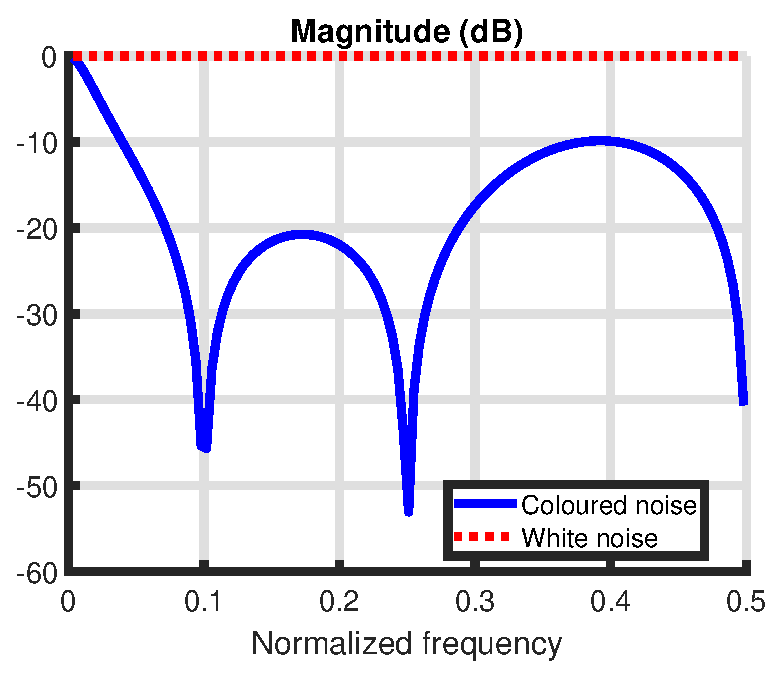
\includegraphics[width=0.6\linewidth]{figures/noise_models.eps}
\caption{Magnitude bode plots of the noise models.}
\label{fig:noise_models}
\end{figure}

\paragraph{Optimization strategies}
As explained in the previous sections, there are multiple ways to find the optimal controller. 

First, the optimal $\rho$ for a certain frequency resolution $f_s/N$ can be found by minimizing $(\ref{eq:JFD})$ and by replacing $\hat{G}(\Omega_k)$ with the actual system $G(\Omega_k)$. This can be done because we are working in a simulation. Note however, that we are optimizing the convex cost function. If the reference model $M$ is realizable, then $J_{mr}(\rho^*) = J(\rho^*) = 0$, which means that, in the noiseless case, the parameters $\rho$ that minimize the convex cost function will also minimize the original cost function. This is not the case any more if the reference model is not realizable.

The TD method consists of minimizing (\ref{eq:JNl1}) w.r.t. $\rho$. However, the parameter $l_1$ must be chosen by the user. The maximum value that can be chosen for $l_1$ is $N/2$. 

The FD method consists of minimizing (\ref{eq:JFD}) w.r.t. $\rho$. The $l_1$-trick can also be used here by minimizing 
\begin{equation}
\boxed{
J_{N,l_1}(\rho) = \frac{1}{N^2}\sum_{n=0}^{l_1} h(n,\rho)^2}
\label{eq:JNl1_FD}
\end{equation}
with $h(n,\rho)$ being the IDFT of $H(\Omega_k,\rho)$. Notice that when $l_1 = N - 1$, $J_{N,l_1}(\rho) = J_N(\rho)$ in the FD.

Finally, the WNLS method will also be used by minimizing (\ref{eq:JWNLS}). This cost function will be minimized by using the Gauss-Newton algorithm. The maximum number of iterations is set to 100 and the algorithm is stopped if the relative difference between the previous and the next estimate is smaller than $10^{-10}$ for all $\rho_i$ in $\rho$. An initial estimate for $\rho$ is found by using the FD method with $l_1 = N-1$. As there is no guarantee that this optimization will converge to the global minimum, the optimization will also be started at the optimal $\rho$ for comparison. Of course, this can only be done because we are working in a simulation.


\paragraph{Input}
The input will be a random phase multisine where all harmonics are excited. The RMS of this multisine is 1 and it is repeated for $P=4$ periods. None of the periods are discarded. The number of samples per period is $N=255$. 

\paragraph{Nonparametric estimate}
The FD methods require a nonparametric estimate. Two different nonparametric estimates are used. The first one is without any removal of system and noise transients by using (\ref{eq:nonparametric_simple}). The second way of obtaining a nonparametric estimate is by using the robust LPM with order $R=2$ and degrees of freedom $q^{\mathrm{noise}}=1$. These values were obtained by using the heuristics mentioned in section \ref{sec:choice_order_dof}. Finally, the WNLS method needs the variance of the FRF estimate. This is also obtained via the robust LPM.

\paragraph{Evaluation}
100 noise realizations are simulated. The resulting controllers are compared by evaluating the cost function with the real system $G(\Omega)$. Both the original cost function and the convex cost function are calculated.
\begin{align*}
J_{mr}(\rho) &= \frac{1}{127} \sum_{k=1}^{127} \Big|M(\Omega_k) - \frac{K(\Omega_k,\rho)G(\Omega_k)}{1+K(\Omega_k,\rho)G(\Omega_k)}\Big|^2\\
J(\rho) &= \frac{1}{127} \sum_{k=1}^{127} \Big|(1-M(\Omega_k))\big[M(\Omega_k) - (1-M(\Omega_k))K(\Omega_k,\rho)G(\Omega_k)\big]\Big|^2
\end{align*}
where $\rho$ is obtained by optimization for one noise realization with any of the methods. Note that $F(\Omega_k)=1$ in the above equations. The sum starts at 1 because DC is not excited by the input. The sum ends at 127 because there are 127 excited harmonics in the input. Then the cost of the controllers obtained from the different noise realizations can be averaged.
\begin{align*}
\Bar{J}_{mr} &= \frac{1}{100} \sum_{i=1}^{100} J_{mr}(\rho^{(i)})\\
\Bar{J} &= \frac{1}{100} \sum_{i=1}^{100} J(\rho^{(i)})
\end{align*}
where $\rho^{(i)}$ are the parameters obtained by optimizing the cost corresponding to the \mbox{$i$-th} noise realization with one of the optimization methods. Note that TD methods with different values of $l_1$ are considered different and shouldn't be mixed up when taking the mean. Finally, the mean cost function can be expressed in decibels.
\begin{align*}
\Bar{J}_{mr}|_{dB} &= 10 \log_{10}(\Bar{J}_{mr}) \\
\Bar{J}|_{dB} &= 10 \log_{10}(\Bar{J})
\end{align*}

\newpage

\subsection{Simple system}
\paragraph{Influence of $\mathbf{l_1}$}
Let's start by seeing how the choice of $l_1$ influences the performance of the resulting controller. The simple system is simulated with disturbing white output noise as explained above. For the TD method, all values of $l_1$  between 1 and $\lfloor N/2 \rfloor = 127$ are tried for each noise realization. For the FD method, all values of $l_1$ between 1 and $N-1 = 254$ are tried for each noise realization. 
The resulting closed loop systems that are obtained by applying the FD method with $l_1 = 1,17  \text{ and } 254$ are shown in figure \ref{fig:CL_FD_simple_flat}. The closed loop system resulting from $l_1=1$ performs poorly and doesn't get close to the reference model $M$. The result is better when $l_1 = 254$, but is best when $l_1 = 17$.

\begin{figure}[H]
\centering
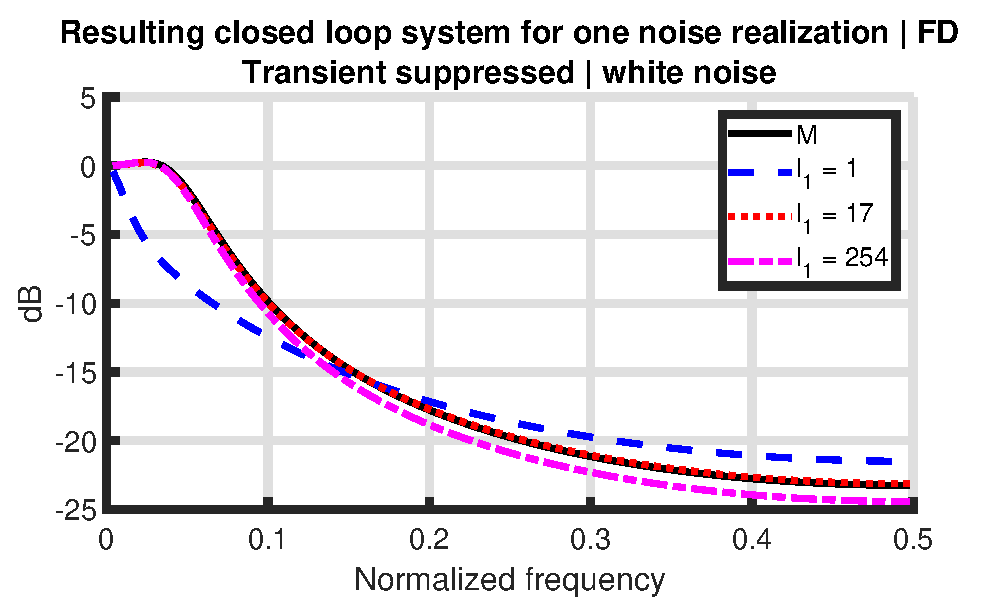
\includegraphics[width=0.6\textwidth]{figures/CL_FD_simple_flat.eps}
\caption{Resulting CL systems for one white noise realization by applying the FD method with different values of $l_1$.}
\label{fig:CL_FD_simple_flat}
\end{figure}

\newpage
The mean cost function for the TD and FD methods for different values of $l_1$ are shown in figure \ref{fig:mean_cost_function_simple_flat}. The mean cost function has a bowl shape as a function of $l_1$. This is because too much information is thrown away when taking a too small $l_1$. However, taking a large $l_1$ just increases the bias. This was also observed in the figure \ref{fig:CL_FD_simple_flat}. One more thing to note is that the original cost function $J_{mr}$ coincides with the convex cost function $J$ most of the time. This means that the sensitivity function can be approximated quite well by the ideal sensitivity function. The cost functions don't coincide for the FD method when $l_1=1$. This is because the resulting closed loop system doesn't come very close to the reference model $M$, as can be seen figure \ref{fig:CL_FD_simple_flat}.

\begin{figure}[H]
\centering
\begin{subfigure}{0.6\textwidth}
	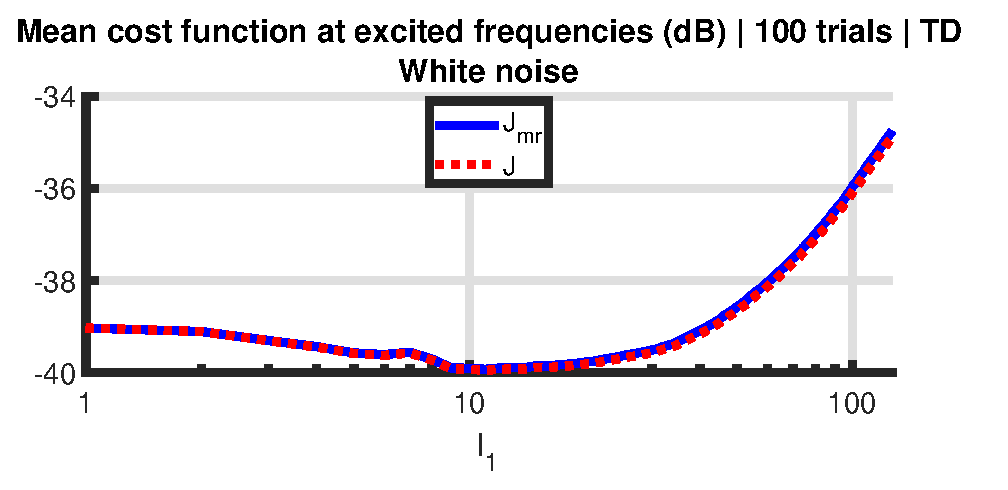
\includegraphics[width=\linewidth]{figures/mean_cost_function_TD_simple_flat.eps}
	\caption{TD method for different $l_1$.}
\end{subfigure}

\begin{subfigure}{0.6\textwidth}
	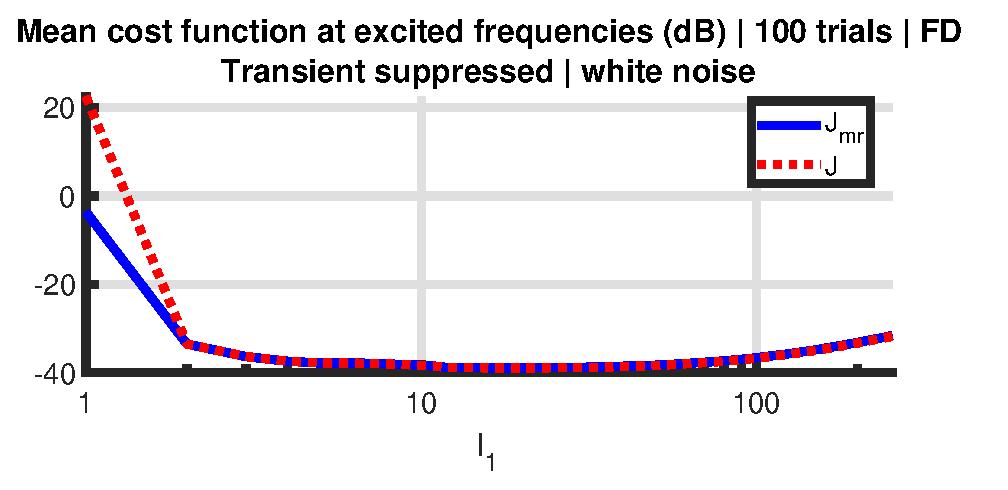
\includegraphics[width=\linewidth]{figures/mean_cost_function_FD_simple_flat.eps}
	\caption{FD method for different $l_1$ and suppression of the transient.}
\end{subfigure}
\caption{Mean cost functions for 100 noise realizations, applied to the simple system with a white noise model.}
\label{fig:mean_cost_function_simple_flat}
\end{figure}

\paragraph{Transient suppression}
In the previous experiment, the transient was suppressed by using the robust LPM. What will happen if the transient is not suppressed? The mean cost function obtained when applying the FD methods with $l_1=254$ with and without transient suppression are given in table \ref{tab:simple_flat_FD_transient_with_without}. Not suppressing the transient gives better results. This is to be expected as the simple system has a very low transient. Moreover, there are no noise transients because the noise is white.
    
\begin{table}[H]
\centering
\begin{tabular}{|ccc|}
\hline
&&\\[-2.5ex]
Method & $\Bar{J}|_{dB}$ & $\Bar{J_{mr}}|_{dB}$ \\
\hline
Transient suppressed & -31.74 & -31.57\\
Transient not suppressed & \textbf{-34.86} & \textbf{-34.73}\\
\hline
\end{tabular}
\caption{FD method with $l_1= 254$ applied to simple system with white noise. With and without transient suppression.}
\label{tab:simple_flat_FD_transient_with_without}
\end{table}

\newpage
Let's see what happens when the output is disturbed by coloured noise. The results of the same experiment, but with coloured noise are shown in table \ref{tab:simple_cololoured_FD_transient_with_without}. The results for coloured noise are better than the results for white noise (table \ref{tab:simple_flat_FD_transient_with_without}). However, this is an unfair comparison as the SNR is not the same in both experiments (see figure \ref{fig:noise_models}). This time, not suppressing the transient is still better.

\begin{table}[H]
\centering
\begin{tabular}{|ccc|}
\hline
&&\\[-2.5ex]
Method & $\Bar{J}|_{dB}$ & $\Bar{J_{mr}}|_{dB}$ \\
\hline
Transient suppressed & -50.99 &-50.98\\
Transient not suppressed & \textbf{-52.51} & \textbf{-52.52}\\
\hline
\end{tabular}
\caption{FD method with $l_1= 254$ applied to simple system with coloured noise. With and without transient suppression.}
\label{tab:simple_cololoured_FD_transient_with_without}
\end{table}


To see why this is the case, we can look at the mean squared error (MSE) of the nonparametric estimate of the transfer function over all the noise realizations. This is plotted in figure \ref{fig:MSE_Gest_simple_coloured}. The estimate with transient removal is better around the transmission zeros of the noise model. To understand why this is so, let's assume that the noise model is given by
\begin{equation*}
	S_y(q^{-1}) = \frac{C(q^{-1})}{D(q^{-1})}
\end{equation*}
In that case, the contribution of the noise on the output at the $k$-th bin is
\begin{equation*}
	\frac{C(\Omega_k)}{D(\Omega_k)} E(k) + \frac{I_E(\Omega_k)}{D(\Omega_k)} = \frac{C(\Omega_k) E(k) + I_E(\Omega_k)}{D(\Omega_k)}
\end{equation*}
with $E(k)$ being the DFT of $e(n)$ and $I_E(\Omega_k)$ being a polynomial in $\Omega_k$ that depends on the initial and end conditions of $e(n)$. When $C(\Omega_k)$ is small, the contribution of the noise is mainly attributed to the transient term $\frac{I_E(\Omega_k)}{D(\Omega_k)}$. Thus, the transient term is dominant at transmission zeros of the noise model. However, at the other frequencies where the random term $\frac{C(\Omega_k)}{D(\Omega_k)} E(k)$ is dominant, the estimate of the FRF is slightly worse (around 1 dB) when taking the transient into account. As the optimization takes all the frequency bins into account, an improvement around the transmission zeros is not enough to improve the estimate of the optimal controller in this case.

\begin{figure}[H]
\centering
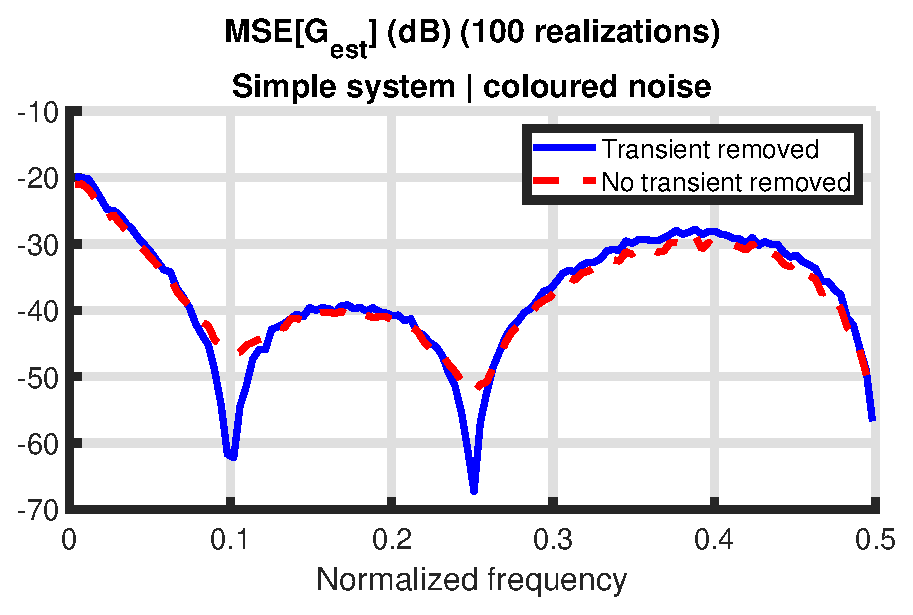
\includegraphics[width=0.6\textwidth]{figures/MSE_Gest_simple_coloured.eps}
\caption{MSE error of the nonparametric estimate of the simple system in the presence of coloured noise with and without transient suppression.}
\label{fig:MSE_Gest_simple_coloured}
\end{figure}

\newpage
\paragraph{TD vs. FD vs. WNLS}
Let's now compare the TD, FD and WNLS methods. For the FD method, the transient can be either suppressed or not taken into account. The WNLS method also uses a nonparametric estimate of the FRF, so here the transient can also be suppressed or not taken into account. Additionally, this optimization needs an initial estimate. As we are working in simulation, the actual parameters $\rho$ that minimize the convex cost function are known. If these parameters are used as initial estimate, we refer to this optimization as ``actual init''. If the estimate of the controller parameters obtained by optimizing using the FD method with $l_1 = 254$ are used as initial estimate, then we refer to this optimization as ``LS init''. The reason for referring to this initial estimate as ``LS init'' is because it is obtained by minimizing the numerator of (\ref{eq:JWNLS}), which is equivalent to minimizing (\ref{eq:JFD}). The numerator of (\ref{eq:JWNLS}) is the sum of squares, which is why the result of this optimization is referred to as the least squares (LS) solution. Table \ref{tab:simple_white_transient_with_without_TD_vs_FD_vs_WNLS} compares the mean cost function of all the methods on the simple system with additive white noise. For the first 3 rows, the parameters $l_1$ that performs the best are shown. The FD method with $l_1 = 23$ where the transient is not suppressed performs best. Moreover, the WNLS method achieves exactly the same results when using the ``LS init'' or the ``actual init''. This means that the ``LS init'' is a good initial estimate for the optimization.

\begin{table}[H]
\centering
\begin{tabular}{|ccc|}
\hline
&&\\[-2.5ex]
Method & $\Bar{J}|_{dB}$ & $\Bar{J_{mr}}|_{dB}$ \\
\hline
TD ($l_1 = 11$) & -39.95 & -39.92 \\
FD transient not suppressed ($l_1 = 23$) & \textbf{-40.03} & \textbf{-40.01} \\
FD transient suppressed ($l_1 = 17$) & -38.95 & -38.92 \\
WNLS transient not suppressed (LS init) & -37.25 & -37.34 \\
WNLS transient not suppressed (actual init) & -37.25 & -37.34 \\
WNLS transient suppressed (LS init) & -37.96 & -37.96 \\
WNLS transient suppressed (actual init) & -37.96 & -37.96 \\
\hline
\end{tabular}
\caption{Simple system with white noise. With and without transient suppression for the FD and WNLS methods. For the first 3 rows, the parameters $l_1$ that yielded the best results are displayed.}
\label{tab:simple_white_transient_with_without_TD_vs_FD_vs_WNLS}
\end{table}

Table \ref{tab:simple_white_transient_with_without_TD_vs_FD_vs_WNLS} showed the results for additive white noise. What will happen if the output is perturbed by coloured noise?  The results for this experiment are shown in table \ref{tab:simple_coloured_transient_with_without_TD_vs_FD_vs_WNLS}. The TD method now performs better than the FD method. However, the WNLS method outperforms the other methods in this case by a large margin. Additionally, even though the WNLS method without transient suppression is better than the other methods, the WNLS method with transient suppression gives a very large improvement. Also, using the ``LS init'' yields exactly the same result as using the ``actual init''.

\begin{table}[H]
\centering
\begin{tabular}{|ccc|}
\hline
&&\\[-2.5ex]
Method & $\Bar{J}|_{dB}$ & $\Bar{J_{mr}}|_{dB}$ \\
\hline
TD ($l_1 = 7$) & -53.46 & -53.46 \\
FD transient not suppressed ($l_1 = 12$) & -52.62 & -52.64 \\
FD transient suppressed ($l_1 = 12$) & -52.31 & -52.31 \\
WNLS transient not suppressed (LS init) & -57.04 & -57.04 \\
WNLS transient not suppressed (actual init) & -57.04 & -57.04 \\
WNLS transient suppressed (LS init) & \textbf{-69.64} & \textbf{-69.64} \\
WNLS transient suppressed (actual init) & \textbf{-69.64} & \textbf{-69.64} \\
\hline
\end{tabular}
\caption{Simple system with coloured noise. With and without transient suppression for the FD and WNLS methods. For the first 3 rows, the parameters $l_1$ that yielded the best results are displayed.}
\label{tab:simple_coloured_transient_with_without_TD_vs_FD_vs_WNLS}
\end{table}

\newpage
The reason why the WNLS method works better for coloured noise than for white noise is that the FRF estimate at all bins are equally noisy when the output is perturbed by white noise. Thus, using a weighting doesn't improve the quality of the controller. However, if the noise is highly coloured, the WNLS method will be more inclined to use the frequency bins where the noise is low to design a controller.

\subsection{Long transient system}
The long transient system is excited with the same signal as before (see section \ref{sec:DT_simulations_introduction}). The output is perturbed with additive white Gaussian noise. Again all values of $l_1$ between 1 and 127 are tried in the TD method and all values of $l_1$ between 1 and 254 are tried for the FD method. Additionally, the transient is either suppressed or not taken into account when estimating a nonparametric representation of the FRF. Finally, the WNLS method is also used to design the controller. A summary of the results is shown in table \ref{tab:long_transient_white_transient_with_without_TD_vs_FD_vs_WNLS}. In this case, the WNLS method with transient suppression gives the best results even though the output is perturbed by white noise. This wasn't the case for the simple system (table \ref{tab:simple_white_transient_with_without_TD_vs_FD_vs_WNLS}). 
%One thing to note is that the mean cost function is very high for the WNLS method where the transient is not suppressed with ``LS init'' as initial estimate. 
%This is because 1 of the 100 optimizations didn't converge to a minimum, causing the mean cost function to grow significantly.
One thing to note is that 1 of the 100 optimizations didn't converge to a minimum for the WNLS method where the transient is not suppressed with ``LS init'' as initial estimate. The failed optimization is not taken into account when calculating the mean cost function.
This shows that there is no guarantee of convergence to a global minimum when minimizing a non-convex cost function. Another interesting thing to note is that the FD method works better when the transient is suppressed, which wasn't the case for the simple system (tables \ref{tab:simple_white_transient_with_without_TD_vs_FD_vs_WNLS} and \ref{tab:simple_coloured_transient_with_without_TD_vs_FD_vs_WNLS}). This is expected as this system has a much longer transient than the simple system. Finally, the FD method with transient suppression achieves the best results when $l_1 = 102$. For the simple system the best results with the FD method were achieved with $l_1 = 23$ and $l_1 = 12$ for white and coloured noise respectively. This shows that more samples of the impulse response $h(n,\rho)$ are needed when the impulse response of the system $G(\Omega)$ is longer. In figure \ref{fig:impulse_simple_long} the impulse responses of the simple and the long transient systems are plotted. It is clear from this figure that $l_1$ should be taken bigger for the long transient system. 

\begin{table}[H]
\centering
\begin{tabular}{|ccc|}
\hline
&&\\[-2.5ex]
Method & $\Bar{J}|_{dB}$ & $\Bar{J_{mr}}|_{dB}$ \\
\hline
TD ($l_1 = 7$) & -54.06 & -54.06 \\
TD ($l_1 = 127$) &  -52.83 & -52.85 \\
FD transient not suppressed ($l_1 = 8$) & -46.71 & -46.66 \\
FD transient not suppressed ($l_1 = 254$) & -45.25 & -45.16 \\
FD transient suppressed ($l_1 = 102$) & -52.80 & -52.80 \\
FD transient suppressed ($l_1 = 254$) & -50.90 & -50.92 \\
WNLS transient not suppressed (LS init) & \textcolor{red}{-50.50 [1 failed]} & \textcolor{red}{-50.48 [1 failed]} \\
WNLS transient not suppressed (actual init) & -50.54 & -50.51 \\
WNLS transient suppressed (LS init) & \textbf{-59.10} & \textbf{-59.11} \\
WNLS transient suppressed (actual init) & \textbf{-59.10} & \textbf{-59.11} \\
\hline
\end{tabular}
\caption{Long transient system with white noise. With and without transient suppression for the FD and WNLS methods. For the first, third and fifth rows, the parameters $l_1$ that yielded the best results are displayed.}
\label{tab:long_transient_white_transient_with_without_TD_vs_FD_vs_WNLS}
\end{table}

\begin{figure}[H]
\centering
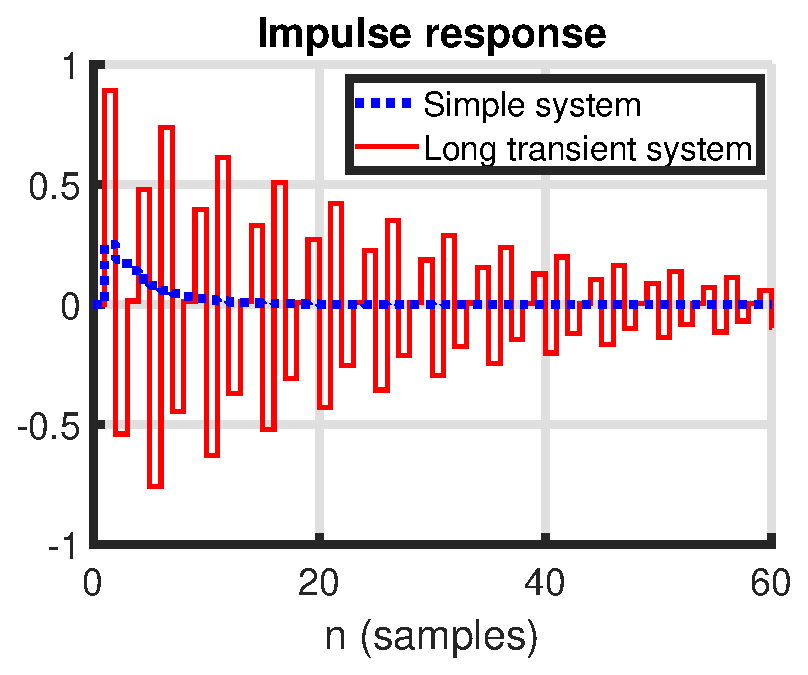
\includegraphics[width = 0.6\textwidth]{figures/impulse_response_simple_long}
\caption{Impulse response of the simple system and the long transient system.}
\label{fig:impulse_simple_long}
\end{figure}

The same experiment can be repeated with coloured noise. The summary of the results is shown in table \ref{tab:long_transient_coloured_transient_with_without_TD_vs_FD_vs_WNLS}. The same conclusions taken for the results of table \ref{tab:long_transient_white_transient_with_without_TD_vs_FD_vs_WNLS} can be applied here. One difference is that in this case, all the 100 optimizations failed for the WNLS method where the transient is not suppressed with ``LS init'' as initial estimate.
\begin{table}[H]
\centering
\begin{tabular}{|ccc|}
\hline
&&\\[-2.5ex]
Method & $\Bar{J}|_{dB}$ & $\Bar{J_{mr}}|_{dB}$ \\
\hline
TD ($l_1 = 2$) & -65.88 & -65.88 \\
TD ($l_1 = 127$) & -64.32 & -64.32 \\
FD transient not suppressed ($l_1 = 2$) & -50.83 & -50.81 \\
FD transient not suppressed ($l_1 = 254$) & -44.76 & -44.67 \\
FD transient suppressed ($l_1 = 133$) & -63.08 & -63.08 \\
FD transient suppressed ($l_1 = 254$) & -62.82 & -62.83 \\
WNLS transient not suppressed (LS init) & \textcolor{red}{[all failed]} & \textcolor{red}{[all failed]}   \\
WNLS transient not suppressed (actual init) & -64.71 & -64.71 \\
WNLS transient suppressed (LS init) & \textbf{-82.73} & \textbf{-82.73} \\
WNLS transient suppressed (actual init) & \textbf{-82.73} & \textbf{-82.73} \\
\hline
\end{tabular}
\caption{Long transient system with coloured noise. With and without transient suppression for the FD and WNLS methods. For the first, third and fifth rows, the parameters $l_1$ that yielded the best results are displayed.}
\label{tab:long_transient_coloured_transient_with_without_TD_vs_FD_vs_WNLS}
\end{table}

\newpage
\subsection{System with non realizable controller}
For the system with non realizable controller, the ideal controller $K^*(\Omega)$ cannot be realized by the proposed controller structure $K(\Omega,\rho)$. Thus, the cost function is strictly greater than 0 for any optimization parameter $\rho$. As was seen in section \ref{sec:WNLS}, this means that the original cost function, convex cost function and WNLS cost function will be minimized for different $\rho$, even in the noiseless case.

\paragraph{Optimal controller}
As we are working in simulation, the FRF of the system $G(\Omega)$ is known exactly. This knowledge can be used to get the optimal controller. The optimal controller was found by minimizing the convex cost function (\ref{eq:JFD}) while replacing the estimate of the FRF of the system $\hat{G}(\Omega_k)$ with the exact FRF of the system $G(\Omega_k)$. Note that the optimal controller will depend on the frequency resolution $f_s/N$ that the user chooses. In this case $N = 255$ as in the previous experiments. One could also minimize the original cost function (\ref{eq:Jmr}). However, we assume that the approximation made to attain the convex cost function is good enough to make little difference. The closed loop system resulting from the optimal controller is shown in figure \ref{fig:non_realizable_optimal}. If the ideal controller $K^*(\Omega)$ is realizable by the proposed controller structure $K(\Omega,\rho)$, then the closed loop system $\mathrm{CL}(\Omega)$ resulting from this noiseless optimization should be exactly equal to the reference system $M(\Omega)$. As the resulting closed loop system does not coincide with the reference model in the figure, it is evident that the reference system $M(\Omega)$ cannot be realized by the proposed controller structure $K(\Omega,\rho)$.

\begin{figure}[H]
\centering
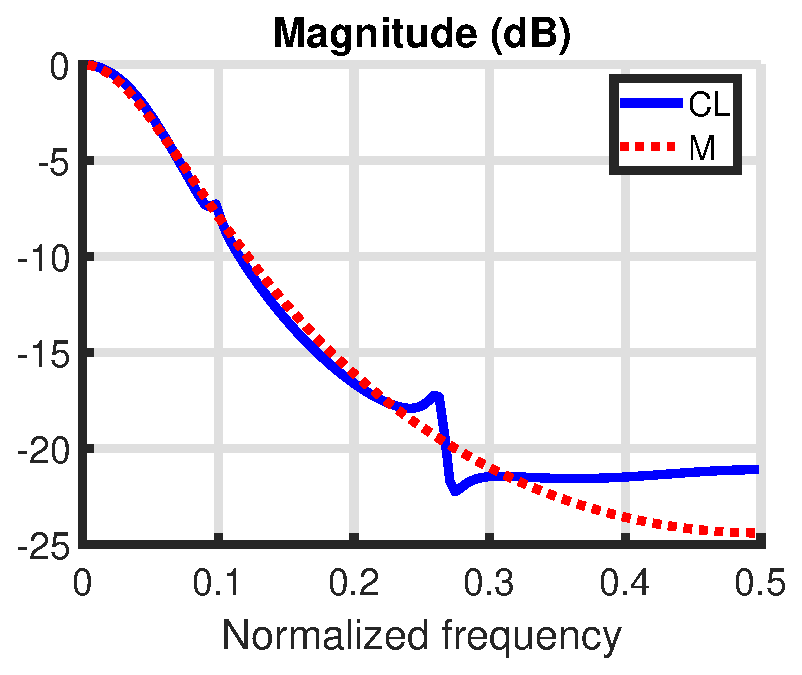
\includegraphics[width = 0.6\textwidth]{figures/undermodeled_optimal}
\caption{Reference system for the system with non realizable controller and the optimal closed loop system.}
\label{fig:non_realizable_optimal}
\end{figure}

\newpage
\paragraph{White noise}
The output is perturbed by Gaussian white noise. The results of this experiment are shown in table \ref{tab:non_realizable_white_transient_with_without_TD_vs_FD_vs_WNLS}. As expected, the optimal controller attains the best results. Notice that the cost function is not zero as the reference model is not realizable by the proposed controller structure. Note also that the convex cost $J$ (-32.49 dB) is almost equal to the original cost $J_{mr}$ (-32.48 dB). This indicates that the approximation made to attain the convex cost function is a good approximation. Additionally, the WNLS method does not perform better in this case. Moreover, the WNLS method fails when the transient is suppressed. 93 of the 100 optimizations fail when using the ``LS init'' as initial estimate. 2 of the optimizations failed when using the ``actual init'' as initial estimate. Finally, the best results are attained when using the FD method with $l_1 =  57$ without transient suppression.

\begin{table}[H]
\centering
\begin{tabular}{|ccc|}
\hline
&&\\[-2.5ex]
Method & $\Bar{J}|_{dB}$ & $\Bar{J_{mr}}|_{dB}$ \\
\hline
Optimal                                     & \textcolor{blue}{-32.49} & \textcolor{blue}{-32.48} \\
TD ($l_1 = 52$)                               & -32.30 & -32.31 \\
TD ($l_1 = 127$)                            & -32.11 & -32.13 \\
FD transient not suppressed ($l_1 = 57$)      & \textbf{-32.34} & \textbf{-32.35} \\
FD transient not suppressed ($l_1 = 254$)   & -32.08 & -32.10 \\
FD transient suppressed ($l_1 = 52$)          & -32.30 & -32.30 \\
FD transient suppressed ($l_1 = 254$)       & -31.75 & -31.78 \\
WNLS transient not suppressed (LS init)     & -31.03 & -31.01 \\
WNLS transient not suppressed (actual init) & -31.03 & -31.01 \\
WNLS transient suppressed (LS init)         & \textcolor{red}{-30.95 [93 failed]}    & \textcolor{red}{-30.93 [93 failed]}    \\
WNLS transient suppressed (actual init)     & \textcolor{red}{-30.96 [2 failed]} & \textcolor{red}{-30.93 [2 failed]} \\

\hline
\end{tabular}
\caption{System with non realizable controller with white noise. With and without transient suppression for the FD and WNLS methods. For the second, fourth and sixth rows, the parameters $l_1$ that yielded the best results are displayed.}
\label{tab:non_realizable_white_transient_with_without_TD_vs_FD_vs_WNLS}
\end{table}

\newpage
\paragraph{Coloured noise}
The same experiment is performed with coloured noise. The results are shown in table \ref{tab:non_realizable_coloured_transient_with_without_TD_vs_FD_vs_WNLS}. The optimal controller performs the best as expected. This optimal controller is available to us because we are working in simulation. Next, the WNLS method without transient suppression results in the worst controllers. 32 of the 100 optimizations failed for the WNLS method with transient suppression when using the ``LS'' init as initial estimate. 25 optimization failed when using the ``actual init'' as initial estimate. Finally, the TD method with $l_1 = 118$ performs the best. Another thing to note is that the FD method with transient suppression works better than the FD method without transient suppression. This wasn't the case when the output was perturbed with white noise (table \ref{tab:non_realizable_white_transient_with_without_TD_vs_FD_vs_WNLS}). This shows that taking the noise transients into account can give us better results.
 
\begin{table}[H]
\centering
\begin{tabular}{|ccc|}
\hline
&&\\[-2.5ex]
Method & $\Bar{J}|_{dB}$ & $\Bar{J_{mr}}|_{dB}$ \\
\hline
Optimal                                     & \textcolor{blue}{-32.4885} & \textcolor{blue}{-32.4837} \\
TD ($l_1 = 118$)                               & \textbf{-32.4709} & \textbf{-32.4676} \\
TD ($l_1 = 127$)                            & -32.4707 & -32.4675 \\
FD transient not suppressed ($l_1 = 221$)      & -32.4623 & -32.4603 \\
FD transient not suppressed ($l_1 = 254$)   & -32.4620 & -32.4602 \\
FD transient suppressed ($l_1 = 118$)          & -32.4685 & -32.4648 \\
FD transient suppressed ($l_1 = 254$)       & -32.4658 & -32.4631 \\
WNLS transient not suppressed (LS init)     & -30.3885 & -30.3817 \\
WNLS transient not suppressed (actual init) & -30.3885 & -30.3817 \\
WNLS transient suppressed (LS init)         & \textcolor{red}{-29.85 [32 failed]}      & \textcolor{red}{-29.81 [32 failed]}       \\
WNLS transient suppressed (actual init)     & \textcolor{red}{-29.72 [25 failed]}       & \textcolor{red}{-29.66 [25 failed]}       \\
\hline
\end{tabular}
\caption{System with non realizable controller with coloured noise. With and without transient suppression for the FD and WNLS methods. For the second, fourth and sixth rows, the parameters $l_1$ that yielded the best results are displayed.}
\label{tab:non_realizable_coloured_transient_with_without_TD_vs_FD_vs_WNLS}
\end{table}

% \section{Continuous time simulations}

\newpage
\section{Conclusion}
Three different methods were used to design a controller that gets the closed loop system as close as possible to a user-defined reference system $M(\Omega)$: the TD, FD and WNLS methods. The FD and WNLS methods need a nonparametric estimate of the FRF of the system $G(\Omega)$. For this nonparametric estimate the system and noise transients can be suppressed or not taken into account. Additionally, the TD and FD methods can employ the $l_1$-trick that allows for a reduction in bias.

The WNLS method with transient suppression gave the best results when the reference model $M(\Omega)$ can be realized perfectly by the proposed controller structure $K(\Omega,\rho)$. However, there is no guarantee that the optimization will converge to the global minimum. 

Applying the WNLS method when the reference cannot be realized perfectly leads to suboptimal results. In this case, the TD method usually performs better than the FD methods. When the system has a long transient and/or noise transients are present, the FD method performs better when the transient is suppressed. The FD method with transient suppression yielded the best results when the output was perturbed by white noise (table \ref{tab:non_realizable_white_transient_with_without_TD_vs_FD_vs_WNLS}, fourth row). However, when the $l_1$-trick is not used, the TD method works better than the FD method (table \ref{tab:non_realizable_white_transient_with_without_TD_vs_FD_vs_WNLS}, third and fifth rows). We mention this here because it is hard to determine which value of $l_1$ will yield the best results. In the simulations, the FRF of the system $G(\Omega)$ is known exactly, which allows us to compare all values of $l_1$. Thus, when working with real measurements, one would probably just use the maximum value of $l_1$ unless one has some prior knowledge of the system.

Thus we can conclude that the TD method works the best on DT systems, unless the reference model is realizable. If the reference model is realizable, then the WNLS method performs the best. Note however, that the TD method only works on DT systems. If one wants to design an analog controller for a CT system, the TD method will not work. In this sense, the proposed FD method is more general than the TD method.

\begin{subappendices}
\section{Division by auto-power spectrum}
\label{appendix:W_filtering}
In section \ref{sec:corr_based_approach}, the following filter is defined.
\begin{equation*}
    W(q^{-1}) = \frac{F(q^{-1})(1-M(q^{-1}))}{S_{UU}(q^{-1})}
\end{equation*}
with $S_{UU}(q^{-1})$ being a parametric representation of the auto-power spectrum of $u(n)$.

If $u(n)$ is DT filtered white noise $u(n) = S_u(q^{-1}) e_u(n)$ and a parametric representation of $S_u(q^{-1})$ is known, then the auto-power spectrum of $u(n)$ becomes
\begin{equation*}
    S_{UU}(q^{-1}) = S_u(q^{-1}) S_u(q)
\end{equation*}
The zeros of $S_u(q^{-1})$ and $S_u(q)$ have an inverse relationship. If $a$ is a zero of $S_u(q^{-1})$, then $a^{-1}$ is a zero of $S_u(q)$. These zeros then become poles of $W(q^{-1})$. Thus, if $S_u(q^{-1})$ contains zeros that are not on the unit circle, the filter $W(q^{-1})$ will be unstable. And so, applying the filter in the time domain is in general not possible.

\newpage
\section{DFT of cross-correlation}
\label{appendix:DFT_cross}
The circular cross-correlation of two discrete signals $x$ and $y$ is defined by \cite[eq. (2.22) ]{Wang_crosscorrelation}
\begin{equation}
    R_{xy}(\tau) = \sum_{n = 0}^{N-1} \overline{x(n)} y(\text{mod}(n+\tau,N)) 
    \label{eq:R_xy}
\end{equation}
Taking the DFT of (\ref{eq:R_xy}) gives
\begin{align*}
    S_{XY}(k) &= \frac{1}{N}\sum_{\tau = 0}^{N-1} R_{xy}(\tau) e^{-j2\pi k \tau /N} = \frac{1}{N}\sum_{\tau = 0}^{N-1} \sum_{n = 0}^{N-1} \overline{x(n)} y(\text{mod}(n+\tau,N))  e^{-j2\pi k \tau /N}\\
    &= \frac{1}{N}\sum_{n = 0}^{N-1} \overline{x(n)} \sum_{\tau = 0}^{N-1} y(\text{mod}(n+\tau,N))  e^{-j2\pi k \tau /N} \\
    &= \frac{1}{N}\sum_{n = 0}^{N-1} \overline{x(n)} e^{j2\pi k t/N} \sum_{\tau = 0}^{N-1} y(\text{mod}(n+\tau,N))  e^{-j2\pi k (n+\tau) /N}
\end{align*}
The second sum is actually independent of $n$.
\begin{align*}
    \sum_{\tau = 0}^{N-1} y(\text{mod}(n+\tau,N))  e^{-j2\pi k (n+\tau) /N} &= \sum_{\tau = 0}^{N-t-1} y(n+\tau)  e^{-j2\pi k (n+\tau) /N}\\ & + \sum_{\tau = N-t}^{N-1} y(n+\tau-N)  e^{-j2\pi k (n+\tau) /N} \\
    &= \sum_{\tau = 0}^{N-t-1} y(n+\tau)  e^{-j2\pi k (n+\tau) /N}\\ & + \sum_{\tau = -t}^{-1} y(n+\tau)  e^{-j2\pi k (n+\tau+N) /N} \\
    & = \sum_{\tau = -t}^{N-t-1} y(n+\tau)  e^{-j2\pi k (n+\tau) /N}
\end{align*}
In the last step we used the fact that $e^{-j2\pi k (n+\tau+N) /N} = e^{-j2\pi k (n+\tau) /N}$. Now by doing one last substitution we get
\begin{align*}
    \sum_{\tau = 0}^{N-1} y(\text{mod}(n+\tau,N))  e^{-j2\pi k (n+\tau) /N} = \sum_{\tau = 0}^{N-1} y(\tau) e^{-j2\pi k \tau /N}
\end{align*}
This equation is valid because the sum runs over all the samples $0,\ldots,N-1$. Finally, the DFT of the cross-correlation is
\begin{align*}
    S_{XY}(k) &= \frac{1}{N} \overline{\sum_{n = 0}^{N-1} x(n) e^{-j2\pi k t/N}} \sum_{\tau = 0}^{N-1} y(\tau)  e^{-j2\pi k \tau /N} \\
    \Rightarrow S_{XY}(k) &=  N \overline{X(k)} Y(k)
\end{align*}

\newpage
\section{Unstable systems}
\label{appendix:unstable}
Open loop experiments are not practical on unstable systems. If we want to measure the FRF of an unstable system, it will have to be done in closed loop with a stabilizing controller. As discussed in section \ref{sec:feedback}, the danger here is that process noise on the output will be fed back to the input. Not taking the right precautions will lead to an inconsistent nonparametric estimate of the FRF in some cases.

First, a quick summary of the solution given in \cite{Data-driven_model_reference_control} will be discussed. Then it will be shown that a nonparametric estimate of the FRF is again hidden in the maths.

\subsection{Correlation-based approach}
\paragraph{Model}
The set-up shown in figure \ref{fig:unstable_system} is considered. An unstable system $G(q^{-1})$ is stabilized by a controller $K_s(q^{-1})$ in negative feedback. The reference signal $r(n)$ is entered between the controller and the system. The reference signal is assumed to be periodic. The input to the system is $u(n)$ and the output of the system $y(n)$ is perturbed by process noise $v(n)$. The signal $x(n)$ is the reference signal that would be used in the actual closed loop system. However, to keep the notation similar to \cite{Data-driven_model_reference_control}, $x(n)$ is set to 0. The closed loop TF from $x(n)$ to $y(n)$ is
\begin{equation*}
    M_s(q^{-1}) = \frac{K_s(q^{-1}) G(q^{-1})}{1 + K_s(q^{-1}) G(q^{-1})}
\end{equation*}

\begin{figure}[H]
    \centering
    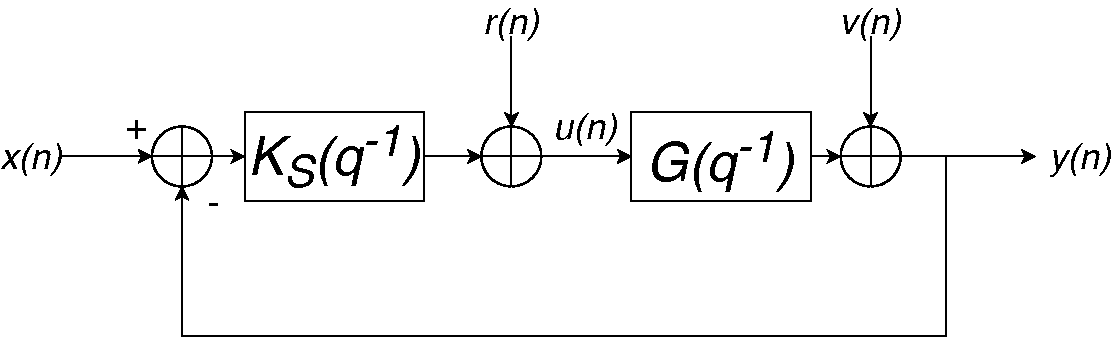
\includegraphics[width = 0.65\textwidth]{figures/unstable_system.pdf}
    \caption{Unstable LTI system with a stabilizing controller in feedback.}
    \label{fig:unstable_system}
\end{figure}

\paragraph{Error signal} The error signal is the same as in section \ref{sec:corr_based_approach}.
\begin{equation*}
    \epsilon(n,\rho) = M u(n) - K(\rho) (1 - M) y(n)
\end{equation*}

\paragraph{Reference filtering}
This time, the reference signal $r(n)$ is filtered instead of the input to the system $u(n)$. The filter $W(q^{-1})$ which is used to obtain $r_W(n)$ is defined differently this time.
\begin{equation}
    W(e^{-j\omega}) = \frac{F(e^{-j\omega}) (1-M(e^{-j\omega}))}{(1-M_s(e^{-j\omega})) S_{RR}(e^{-j\omega})}
    \label{eq:W_unstable_non-practic}
\end{equation}
with $S_{RR}(e^{-j\omega})$ being the auto-power spectrum of the reference signal. It is pointed out in \cite{Data-driven_model_reference_control} that $W(e^{-j\omega})$ cannot be implemented in this way, because $M_s$ is not known as we don't have access to a parametric representation of $G$. This is solved in the following way. First, $u(n)$ is written as a function of $r(n)$ and $v(n)$.
\begin{equation*}
    u(n) = \frac{1}{1+K_s G} r(n) - \frac{K_s}{1+K_s G} v(n)
\end{equation*}
Assuming that there is no noise $v(n) = 0$ and rewriting $1+K_s G$ in terms of $M_s$, gives
\begin{equation*}
    u(n) = (1-M_s) r(n)
\end{equation*}
Hence, there is a relation between the auto-power spectrum of $r(n)$ and the cross-power spectrum between $r(n)$ and $u(n)$.
\begin{equation*}
    S_{RU}(e^{-j\omega}) = (1-M_s(e^{-j\omega})) S_{RR}(e^{-j\omega})
\end{equation*}
And so (\ref{eq:W_unstable_non-practic}) becomes
\begin{equation*}
    W(e^{-j\omega}) = \frac{F(e^{-j\omega}) (1-M(e^{-j\omega}))}{S_{RU}(e^{-j\omega})}
\end{equation*}
$S_{RU}(e^{-j\omega})$ can be estimated from the data and the filter can be applied to $r(n)$ in the FD to obtain $r_W(n)$.

\paragraph{Correlation criterion}
Then, the cross-correlation between $r_W(n)$ and $\epsilon(n,\rho)$ is calculated.
\begin{equation*}
    R_{r_W \epsilon}(\tau,\rho) = \frac{1}{N\!P} \sum_{n=0}^{N\!P-1} r_W(n-\tau) \epsilon(n,\rho)
    % \label{eq:RuWepstau_unstable}
\end{equation*}
with $P$ being the number of periods measured. The cost function can then be calculated by using (\ref{eq:JNl1}).

\subsection{Nonparametric estimate}
The error signal in the FD becomes
\begin{equation*}
    E(kP,\rho) = M(\Omega_k) U(kP) - K(\Omega_k,\rho) (1-M(\Omega_k)) Y(kP)
\end{equation*}
Here, because the reference signal is periodic, the frequencies $\Omega_k$ correspond to the DFT bins $kP$. For the rest of this section, the frequencies $\Omega_k$ will be left out from the equations for clarity.
The filtered reference signal becomes
\begin{equation*}
    R_W(kP) = \frac{F (1-M) R(kP)}{R(kP) \overline{U(kP)}}
\end{equation*}
Then the cross-power spectrum between $\epsilon(n,\rho)$ and $r_W(n)$ is
\begin{align*}
    S_{R_W\!E}(\Omega_k,\rho) &= R_W(kP) \overline{E(kP,\rho)} = F(1-M) \overline{\Big[M \frac{U(kP) \overline{R(kP)}}{U(kP) \overline{R(kP)}} - K(\rho) (1-M) \frac{Y(kP) \overline{R(kP)}}{U(kP) \overline{R(kP)}}\Big]}\\
    &= F(1-M) \overline{[M - K(\rho) (1-M) \hat{G}(\Omega_k) ]}
\end{align*}
with 
\begin{equation}
    \hat{G}(\Omega_k) = \frac{Y(kP) \overline{R(kP)}}{U(kP) \overline{R(kP)}} = \frac{Y(kP)}{U(kP)}
    \label{eq:G=Y(kP)/U(kP)_unstable}
\end{equation}
If $\hat G$ is replaced by the actual system $G$, $S_{R_W\!E}(\Omega_k,\rho)$ is exactly the quantity being integrated over in (\ref{eq:J}). As was discussed in section \ref{sec:corr_based_approach}, (\ref{eq:G=Y(kP)/U(kP)_unstable}) is equivalent to taking the DFT of every period and taking the mean of the spectra over the periods.
\begin{equation*}
    \hat G(\Omega_k) = \frac{\frac{1}{P}\sum_{p=0}^{P-1}  Y^{(p)}(k)}{\frac{1}{P}\sum_{p=0}^{P-1}  U^{(p)}(k)}
\end{equation*}
Note that this estimate is consistent when the excitation is periodic. For arbitrary excitations it is inconsistent. It is interesting to see that the unsimplified fraction in (\ref{eq:G=Y(kP)/U(kP)_unstable}) looks like the indirect method for estimating the FRF (see section \ref{sec:feedback}).
\begin{equation*}
    \hat G(\Omega_k) = \frac{ \frac{1}{P}\sum_{m=0}^P Y^{(m)}(k) \overline{R^{(m)}(k)} } { \frac{1}{P}\sum_{m=0}^P U^{(m)}(k) \overline{R^{(m)}(k)} }
\end{equation*}
This FRF estimate is consistent when using arbitrary excitations.
\end{subappendices}

\counterwithout{figure}{subsection}
\counterwithout{table}{subsection}
\counterwithout{figure}{section}
\counterwithout{table}{section}
\counterwithin{figure}{chapter}
\counterwithin{table}{chapter}
\chapter{Guaranteed stability}
\label{chapter:guaranteed_stability}
\section{Introduction}
Model reference control allows the user to design a controller without the need to estimate a parametric model of the open loop system. However, the stability of the closed loop system is not guaranteed when minimizing (\ref{eq:Jmr}) or (\ref{eq:J}). If a parametric representation of the TF of an LTI system is known, then the stability of the closed loop system can be inferred by analysing the poles of the closed loop system. As long as none of the poles are in the right half plane of the complex plane for CT systems, then the closed loop system is stable. To ensure the stability for DT system, none of the poles are allowed to be outside of the unit circle in the complex plane. In data-driven model reference control, the locations of the poles are unknown, which means we must find another way to guarantee the stability of the closed loop system. The following is a detailed repetition of the idea presented in \cite{Data-driven_model_reference_control}. We will first give a small explanation of the small-gain theorem and will then show how this theorem can be used to guarantee the stability in data-driven model reference control. 
%Finally, this stability constraint will be used to design an analog controller for a real system.

\section{Small-gain theorem}
The small-gain theorem can be seen as a generalization of the Nyquist criterion to nonlinear time-varying system \cite{Zames1966}. Assume that we have an interconnection of 2 stable LTI systems as shown in figure \ref{fig:interconnection}.

\begin{figure}[H]
\centering
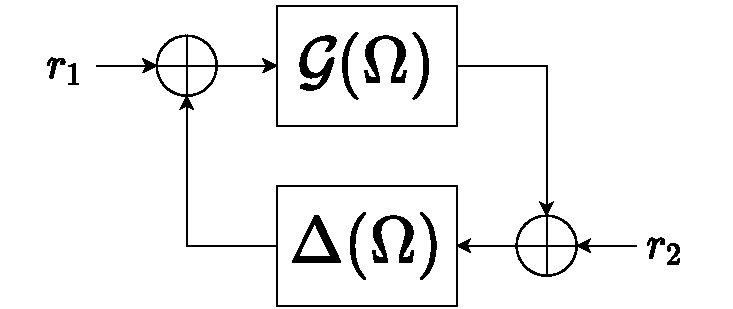
\includegraphics[width = 0.45\textwidth]{figures/interconnection.pdf}
\caption{An interconnection of 2 stable LTI systems.}
\label{fig:interconnection}
\end{figure}

A specific case of the small-gain theorem \cite{control_theory_ljung} states that the interconnection of these two stable LTI systems is stable if 
\begin{equation}
||\mathcal{G}(\Omega)\Delta(\Omega)||_\infty < 1
\end{equation}
with $||\bullet||$ being the H-infinity norm of an LTI system defined as
\begin{equation*}
	||H(\Omega)||_\infty = \begin{cases}
		\sup_\omega |H(j\omega)| & \text{for CT systems} \\
		\sup_\omega |H(e^{j\omega})| & \text{for DT systems} \\
	\end{cases}
\end{equation*}

\paragraph{Example}
Consider a simple example of a CT system being controlled with a proportional controller in negative feedback. 
\begin{align*}
\mathcal{G}(s) &= \frac{1}{s+2}\\
\Delta(s) &= K_P
\end{align*}
Then
\begin{equation}
|\mathcal{G}(j\omega)\Delta(j\omega)|^2 = \Big|\frac{1}{j\omega+2}K_P\Big|^2 = \frac{K_P^2}{\omega^2 + 4}
\label{eq:GDeltasquared}
\end{equation}
The quantity (\ref{eq:GDeltasquared}) must be smaller than 1 for all $\omega \in \mathds{R}$.
\begin{align*}
\Rightarrow &K_P^2 < \omega^2 + 4 \quad \forall \omega \in \mathds{R} \\
\Leftrightarrow  & K_P^2-4 < \omega^2 \quad \forall \omega \in \mathds{R}
\end{align*}
If the above inequality holds for $\omega = 0$, then the above inequality holds for all $\omega \in \mathds{R}$.
\begin{equation}
K_P^2-4 < 0 \Rightarrow \boxed{-2 < K_P < 2}
\label{eq:Kpboundssmallgain}
\end{equation}

According to the small-gain theorem, choosing $K_P$ between -2 and 2 will guarantee the stability of the closed loop system. Let's now compare this result to the traditional way of determining whether the closed loop system is stable: by analysing the location of the closed loop poles. The closed loop system is given by
\begin{equation*}
	\frac{\mathcal{G}(s)}{1 + \mathcal{G}(s)\Delta(s)} = \frac{\frac{1}{s+2}}{1 + \frac{K_P}{s+2}} = \frac{1}{s + 2 + K_P}
\end{equation*}
The location of the closed loop pole is $-(2+K_P)$. To ensure stability, the real part of the pole must be smaller than 0
\begin{equation}
-(2 + K_P) < 0 \Rightarrow \boxed{-2 < K_P}
\label{eq:Kpboundstradition}
\end{equation}
The bounds (\ref{eq:Kpboundssmallgain}) are contained in the bounds (\ref{eq:Kpboundstradition}). Thus, we can conclude that the stability bounds given by the small-gain theorem are much more conservative. For example, choosing $K_P=4$ will still result in a stable closed loop system. The nice thing about the small-gain theorem, is that it is sufficient to have a nonparametric estimate of the FRF of $\mathcal{G}(\Omega)$ and $\Delta(\Omega)$ in order to determine whether the closed loop system will be stable. Contrast this with the need to know the location of the poles of $\mathcal{G}(\Omega)$ to get to (\ref{eq:Kpboundstradition}).

\subsection{Stability constraints}
\label{sec:stability_constraints}
In data-driven model reference control, the user does not have access to a parametric representation of the TF of the system $G(\Omega)$. However, we can estimate the FRF of the system nonparametrically. This nonparametric estimate can be used to guarantee stability by using the small-gain theorem.

Looking back at figure \ref{fig:closed_loop_system}, we can see that $\mathcal{G}(\Omega) = K(\Omega,\rho) G(\Omega)$, $\Delta = 1$, $r_1 = r - v$ and $r_2 = 0$. In order to use the small-gain theorem, $\mathcal{G}$ and $\Delta$ must be stable. As $K(\Omega,\rho)$ is stable by construction, this means that $G(\Omega)$ must be stable. Thus, the stability cannot be guaranteed when $G(\Omega)$ is unstable. If $G(\Omega)$ is stable, then the closed loop system is stable if
\begin{equation*}
||K(\Omega,\rho) G(\Omega)||_\infty < 1
\end{equation*}
The problem with this constraint is that it cannot be realized in practice. The quantity $|K(\Omega,\rho) G(\Omega)|$ must be smaller than 1 for all frequencies. In reality, a nonparametric estimate has a certain frequency resolution $f_s/N$, with $f_s$ being the sampling frequency and $N$ being the number of samples in 1 period of the excitation signal. Thus, the user must ensure that the frequency resolution is high enough to not miss any resonance peaks in the FRF. With this in mind, the constraint turns into
\begin{equation*}
|K(\Omega_k,\rho) \hat{G}(\Omega_k)| < 1 \,, \quad \forall k \in \kexc
\end{equation*}
with $\hat{G}(\Omega_k)$ being the estimate of the FRF of $G(\Omega)$ at the $k$-th DFT bin and $\kexc$ being the set of excited harmonics.

The optimization can then be done in the following way:
\begin{align*}
	&\hat{\rho} = \underset{\rho}{\mathrm{arg\,min}} \, J(\rho) \\
	\text{subject to } &|K(\Omega_k,\rho) \hat{G}(\Omega_k)| < 1 \quad \forall k \in \kexc
\end{align*}
with $J(\rho)$ being the TD cost function (\ref{eq:JNl1}), FD cost function (\ref{eq:JFD}) or the FD cost function with $l_1$-trick (\ref{eq:JNl1_FD}). As the cost function is a convex function and the constraints are convex, the optimization problem as a whole is also convex, meaning that it can be solved with a convex solver.

\subsection{Better stability constraints}
The stability constraints discussed in the previous section are very conservative. We can do better. The closed loop system that is shown in figure \ref{fig:closed_loop_system} can be redrawn as shown in figure \ref{fig:small_gain_CL1}. The reference signal $r$ was grouped together with the output noise $v$ and the controller was split up into 2 branches by using $K(\rho) = (K(\rho) - K^*) + K^*$, with $K^*$ being the ideal controller that might not be realizable by the proposed controller structure $K(\rho)$.

\begin{figure}[H]
\centering
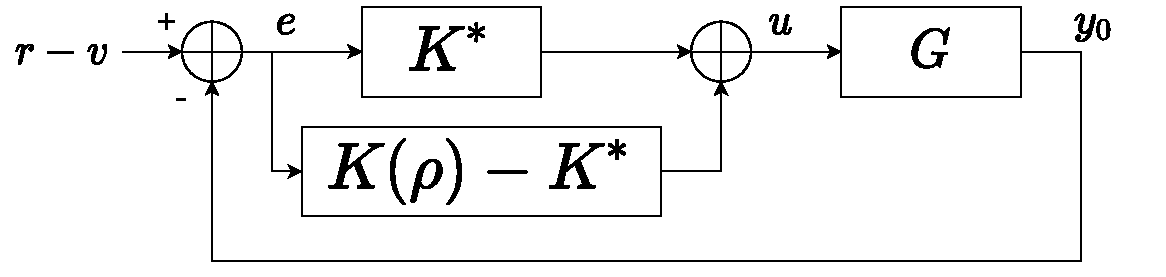
\includegraphics[scale=0.6]{figures/small_gain_CL1}
\caption{Redrawing figure \ref{fig:closed_loop_system} by using $K(\rho) = (K(\rho) - K^*) + K^*$ and by grouping the reference $r$ with the output noise $v$.}
\label{fig:small_gain_CL1}
\end{figure}

The next step involves shifting the system $G(\Omega)$ into the 2 newly created branches. This is shown in figure \ref{fig:small_gain_CL2}.
 
\begin{figure}[H]
\centering
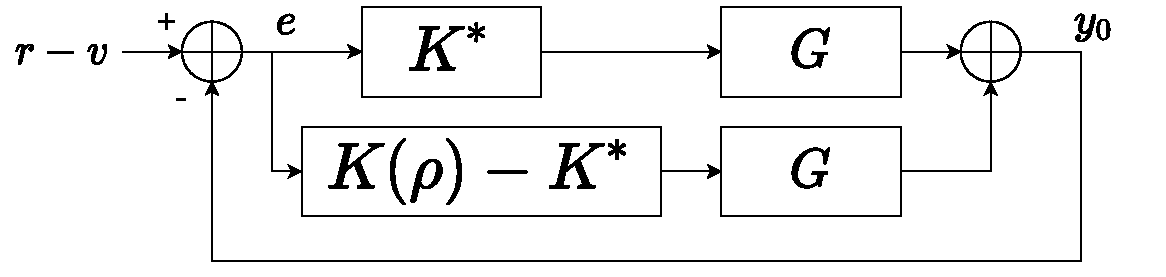
\includegraphics[scale=0.6]{figures/small_gain_CL2}
\caption{Redrawing figure \ref{fig:small_gain_CL1} by shifting $G(\Omega)$ to the left.}
\label{fig:small_gain_CL2}
\end{figure}

Finally, by playing around with the summations we arrive at the block diagram shown in figure \ref{fig:small_gain_CL3}.
\begin{figure}[H]
\centering
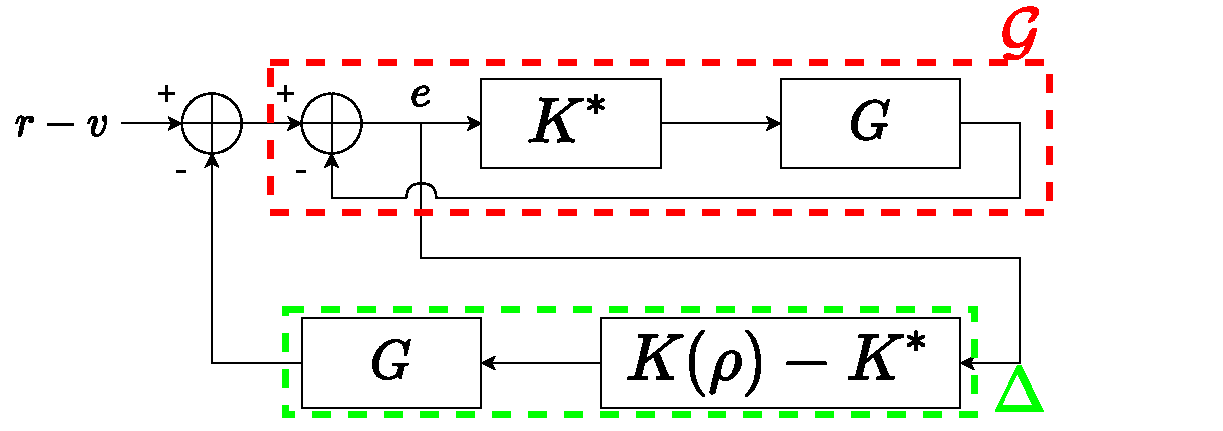
\includegraphics[scale=0.6]{figures/small_gain_CL3}
\caption{Redrawing figure \ref{fig:small_gain_CL2} by playing around with the summations.}
\label{fig:small_gain_CL3}
\end{figure}


With a little bit of imagination, we can see that this is an interconnection of 2 systems.
\begin{align*}
\mathcal{G} &= \frac{1}{1+K^*G} = 1-M\\
\Delta &= (K(\rho)-K^*)G
\end{align*}
The system $\mathcal{G}$ is the TF between the output of the first summer and $e$. To use the small-gain theorem, both $\mathcal{G}$ and $\Delta$ must be stable systems. $\mathcal{G}$ is stable because $M$ is stable by construction. Showing that $\Delta$ is stable is a bit more involved. This is because $K^*$ is not necessarily stable and causal. Using
\begin{equation*}
K^* = \frac{M}{G(1-M)}
\end{equation*}
we can expand $\Delta$
\begin{equation*}
\Delta = K(\rho) G - \frac{M}{G(1-M)} G = K(\rho) G - \frac{M}{1-M}
\end{equation*}
The first term $K(\rho) G$ is stable because $K(\rho)$ is stable by construction and because $G$ is also assumed to be stable. If $G$ is not stable, then the small-gain theorem cannot be used. The second term is not necessarily stable $\frac{M}{1-M}$. However, it can be chosen by the user in such a way that it is stable. The fact that $\frac{M}{1-M}$ must be stable is not mentioned in \cite[Lemma 1]{Data-driven_model_reference_control}. 

Finally, if $\mathcal{G}$ and $\Delta$ are stable, the small-gain theorem says that the stability of the closed loop system is guaranteed if
\begin{align*}
&||\mathcal{G}\Delta||_\infty < 1 \\
\Leftrightarrow & \Big|\Big|(1-M) \big(K(\rho) G - \frac{M}{1-M}\big)\Big|\Big|_\infty < 1 \\
\Leftrightarrow & ||(1-M)K(\rho)G - M||_\infty < 1\\
\Leftrightarrow & ||M -(1-M)K(\rho)G ||_\infty < 1
\end{align*}

The optimization can then be done with these constraints
\begin{align*}
	&\hat{\rho} = \underset{\rho}{\mathrm{arg\,min}} \, J(\rho) \\
	\text{subject to } &|M(\Omega_k) -(1-M(\Omega_k))K(\Omega_k,\rho)\hat{G}(\Omega_k)| < 1 \,, \quad \forall k \in \kexc
\end{align*}
Again, the same rules apply here: the frequency resolution $f_s/N$ must be high enough to not miss any resonance peaks. $J(\rho)$ can be one of the cost function mentioned in section \ref{sec:stability_constraints}. These constraints are also convex, which makes the optimization problem convex. Thus, it can be solved with a convex solver.

These constraints are less conservative than the constraints from section \ref{sec:stability_constraints} for the following reason. If $\hat G$ is replaced by the exact system $G$ and if $K(\rho)$ is replaced by the ideal controller $K^*$ then
\begin{equation*}
M -(1-M)K^*G = M - (1-M)\frac{M}{1-M} = 0
\end{equation*}
which means that the constraints are fulfilled. Thus, $M -(1-M)K(\rho)G$ is a measure of how close the closed loop system is to the stable reference model. This is also evident by noticing that $M -(1-M)K(\rho)G$ is contained inside the convex cost function.
\begin{equation*}
    J(\rho) =  \Big|\Big|F(1-M)) \Big[M-(1-M)K(\rho) G\Big]  \Big|\Big|_2^2 
\end{equation*}

%\section{Conclusion}
%The small-gain theorem was used to derive convex constraints that guarantee the stability of the closed loop system under certain conditions. The FD method was used to design an analog controller for a Wiener-Hammerstein system. The stability constraints were used to guarantee the stability of the closed loop system. Then, the analog controller was constructed successfully. Finally, the analog controller and closed loop system were measured. However, the measurement of the analog controller was not successful. The cause of this failure is unknown.

\counterwithout{figure}{subsection}
\counterwithout{table}{subsection}
\counterwithout{figure}{section}
\counterwithout{table}{section}
\counterwithin{figure}{chapter}
\counterwithin{table}{chapter}
\chapter{Real experiment}
\label{chapter:real_experiment}

\section{Introduction}
The goal of this experiment is to use data-driven model reference control to design an analog controller for a CT system. The open loop system is shown in figure \ref{fig:WH_OL}. It is a Wiener-Hammerstein system. This is a system that consists of a series connection of 2 LTI systems with a nonlinear static system in between them.

\begin{figure}[H]
    \centering
    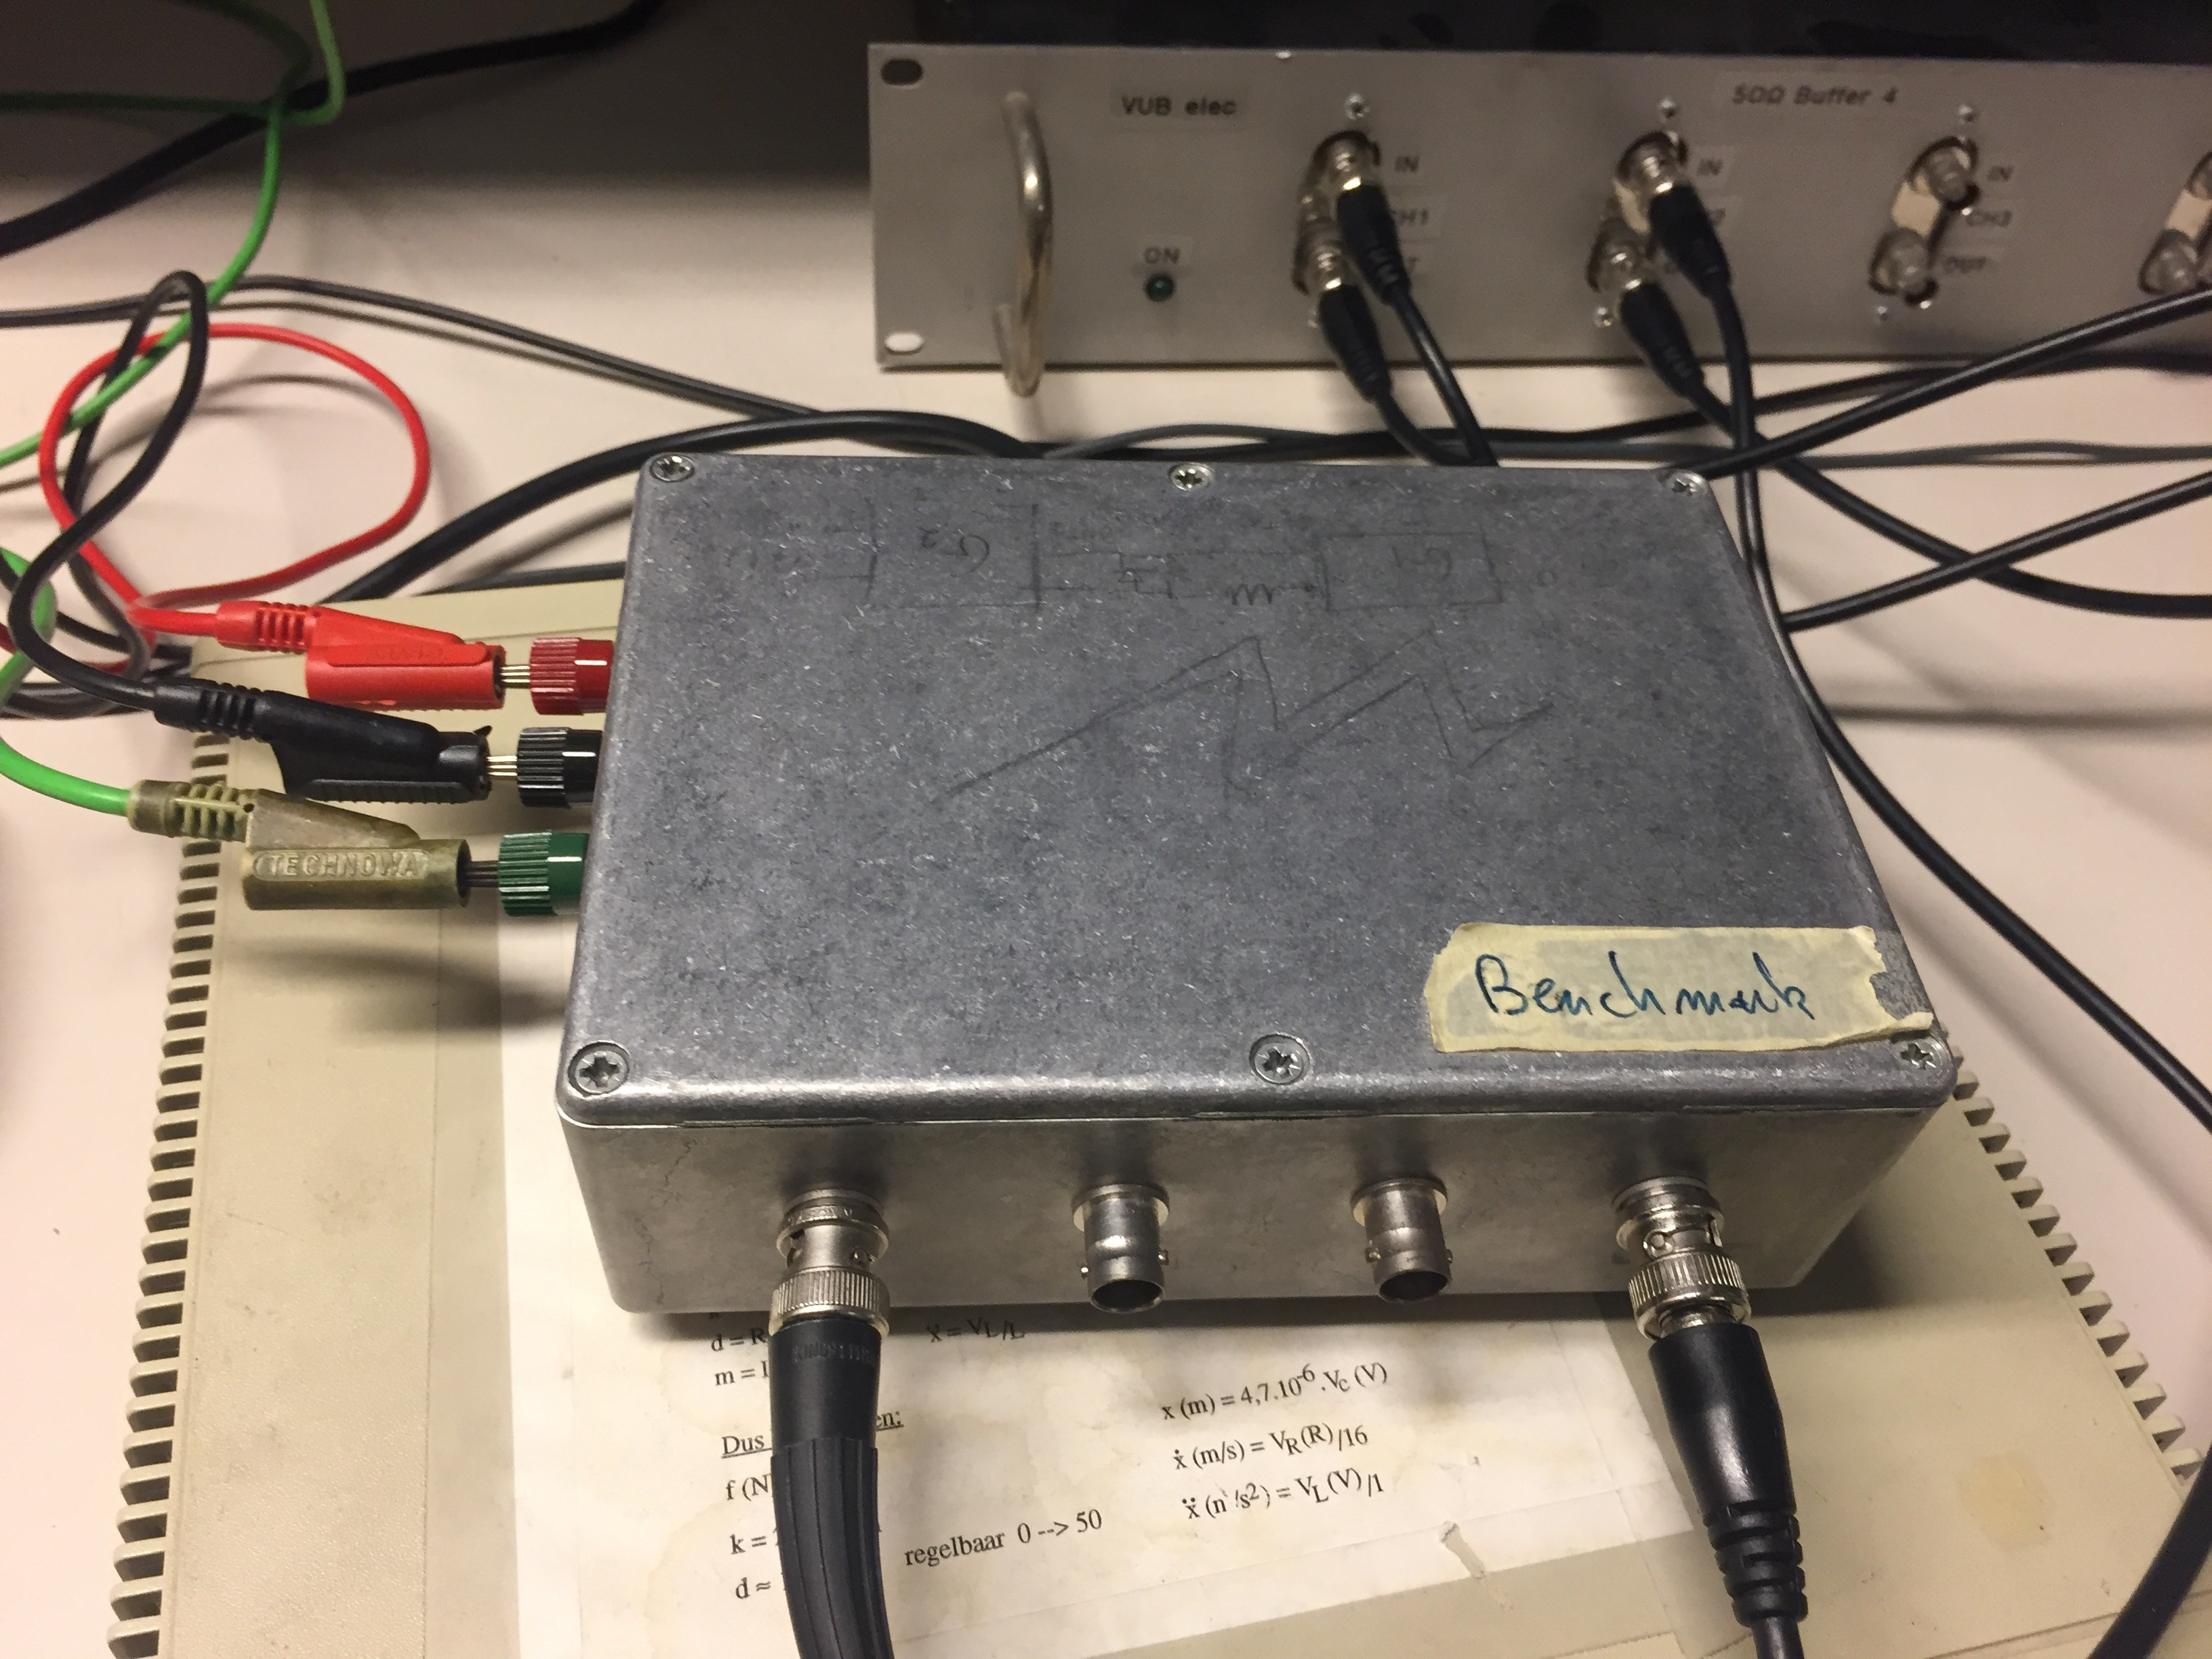
\includegraphics[width = 0.5\textwidth]{figures/DUT.jpg}
    \caption{Picture of the Wiener-Hammerstein system.}
    \label{fig:WH_OL}
\end{figure}


A diagram of the measurement set-up is shown in figure \ref{fig:set-up}. This measurement set-up is a band-limited set-up (section \ref{sec:band-limited}). The device-under-test (DUT) can be the Wiener-Hammerstein system $G(s)$, the controller $K(s)$ or the closed loop system.

\begin{figure}[H]
    \centering
    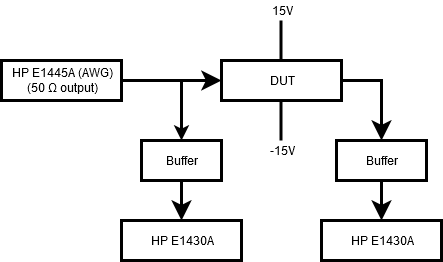
\includegraphics[width = 0.6\textwidth]{figures/DUT_setup.png}
    \caption{Diagram of the measurement set-up}
    \label{fig:set-up}
\end{figure}

\newpage
\subsection{Nonparametric estimate}
\label{sec:nonparametric_estimate_controller}
The first step in this experiment is to get a nonparametric estimate of the FRF of the system $G(s)$. However, the Wiener-Hammerstein system is nonlinear. This means that the system cannot be represented by a TF. However, we can find the best linear approximation (BLA) of the system $G_{\textrm{BLA}}$. With an intelligently designed excitation signal, it is possible to suppress the non-linearities in the input and output signals \cite{pintelon_book}. Neglecting the transient term, we can say that the output spectrum contains 3 contributions if it is excited by an input $U(k)$:
\begin{itemize}
	\item A linear contribution from $G_{\textrm{BLA}}(\Omega_k) U(k)$
	\item A random noise contribution that doesn't depend on the input $N_Y(k)$
	\item A nonlinear distortion term that does depend on the input $Y_S(k)$
\end{itemize}
Thus, we can write
\begin{equation*}
	Y(k) = G_{\textrm{BLA}}(\Omega_k) U(k) + N_Y(k) + Y_S(k)
\end{equation*}
If we apply the input for $P$ periods we get
\begin{equation*}
	Y^{(p)}(k) = G_{\textrm{BLA}}(\Omega_k) U(k) + N_Y^{(p)}(k) + Y_S(k) \,, \quad p = 1,\ldots,P
\end{equation*}
Only the random noise contribution differs from period to period. As the nonlinear distortions depend on the input, they will be the same for every period. In this way, we are blind to the nonlinear distortions. They will remain in our estimate of the best linear approximation $\hat G_{\textrm{BLA}}$ even if we apply the excitation signal for an infinite amount of periods.

The solution to this problem is to design $M$ realizations of the excitation signal. More specifically, in the case of multisine excitations, this means that multiple multisines must be designed with different random phases for every excited harmonic. The amplitude of the sine components can be the same for every realization.
\begin{equation*}
	U^{(m)}(k) = A_k e^{j \phi_k^{(m)}} \,, \quad \phi_k^{(m)} \sim \mathcal{U}(0,2\pi) \,, \quad m = 1,\ldots,M
\end{equation*}
These $M$ different realizations can be applied for $P$ periods. The output spectrum for the $p$-th period of the $m$-th realization is then given by
\begin{equation*}
	Y^{(m,p)}(k) = G_{\textrm{BLA}}(\Omega_k) U^{(m)}(k) + N_Y^{(m,p)}(k) + Y_S^{(m)}(k) 
\end{equation*}
The random noise contribution is different for every period of every realization. The nonlinear distortions are different for every realization. Dividing the output spectrum by the input spectrum gives us a nonparametric estimate of the FRF of $G_{\textrm{BLA}}$ for every period of every realization.
\begin{equation*}
	\hat G^{(m,p)}(\Omega_k) = \frac{Y^{(m,p)}(k)}{U^{(m)}(k)} = G_{\textrm{BLA}}(\Omega_k)  + \frac{N_Y^{(m,p)}(k)}{U^{(m)}(k)} + \frac{Y_S^{(m)}(k)}{U^{(m)}(k)}
\end{equation*}
Now, as a result of applying multiple realizations of the input signal, the nonlinear distortions can be isolated from the linear contributions and suppressed. This results in a better estimate of the FRF of the best linear approximation. 

More information on how to estimate the FRF of the best linear approximation can be found in \cite[Chapter 4]{pintelon_book}. With that said, a multisine was applied to the \mbox{Wiener-Hammerstein} system by using the measurement set-up shown in figure \ref{fig:set-up}. 

\newpage
The excitation signal had the following properties:
\begin{itemize}
\item Sampling frequency: $f_s = 78.125 \,\textrm{kHz}$
\item Samples per period: $N = 2048$
\item Periods per realization: $P = 2$
\item Number of realizations: $M = 20$
\item Excited harmonics: $\kexc = \{k \in \mathbb{N} : 1 \leq k \leq 262\}$
\item Input RMS: $V_{\mathrm{RMS}} = 100 \, \textrm{mV}$
\item Sine component amplitude: $A_k^{(1)} = \ldots = A_k^{(M)} = \text{constant} \,, \quad \forall k \in \kexc$
\item Sine component phases: $\phi_k^{(m)} \sim \mathcal{U}(0,2\pi) \,, \quad m = 1, \ldots, M \,, \quad \forall k \in \kexc$ 
\end{itemize}
The 262-nd harmonic corresponds to the maximum excited frequency
\begin{equation*}
	f_{\mathrm{max}} = 262 \frac{f_s}{N} = 9994.5 \, \mathrm{Hz} \approx 10 \,\textrm{kHz}
\end{equation*}

The measurement set-up automatically waits for the system to be in steady state before taking measurements. However, noise transients can still be present in the input and output spectra. Therefore, the Robust LPM is used to obtain a nonparametric estimate of the FRF of the system at the excited frequencies. Additionally, because multiple realizations are measured, the Robust LPM can discern between the noise variance and the nonlinear distortions. 

Using the heuristics mentioned in section \ref{sec:choice_order_dof}, the order and degrees of freedom best suitable for the Robust LPM can be determined. After applying the Robust LPM for different values of the order and the degrees of freedom, it was observed that increasing either of these parameters doesn't decrease the total estimated variance of the FRF. Thus the default parameters $R=2$ and $q^{\mathrm{noise}}=1$ are used. The nonparametric estimate of the FRF of the best linear approximation of the Wiener-Hammerstein system is shown in figure \ref{fig:GBLA_nonparam}. The nonlinear distortion are clearly dominant over the random noise contributions. This is the reason why $M=20$ realizations were measured.

\begin{figure}[H]
\centering
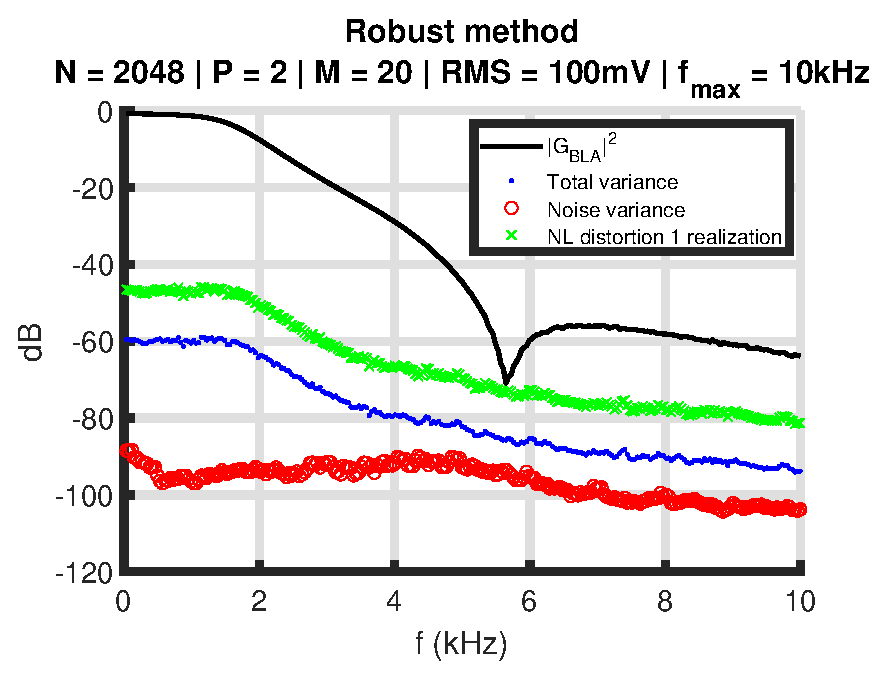
\includegraphics[width = 0.65\textwidth]{figures/robust_method_G.eps}
\caption{Nonparametric estimate of the FRF of the best linear approximation of the Wiener-Hammerstein system.}
\label{fig:GBLA_nonparam}
\end{figure}

\subsection{Controller design}
\label{sec:controller_design_controller}
Now that we have a nonparametric estimate of the FRF of $G_{\textrm{BLA}}(s)$, we can design an analog controller for it.

After experimenting with multiple reference models $M(s)$ and controller structures $K(s,\rho)$, the following resulted in a suitable closed loop system.
\begin{align*}
&M(s) = M_1(s) M_2(s) \\
\text{with } &M_1(s) = \frac{\omega_1^2}{s^2 + 2\omega_1s + \omega_1^2} \,, \quad \omega_1 = 2 \pi \, 5000 \, \mathrm{Hz} \\
\text{and } &M_2(s) = \frac{\omega_2^2}{s^2 + 2\omega_2s + \omega_2^2} \,, \quad \omega_2 = 2 \pi \, 8000 \, \mathrm{Hz} \\
&K(s,\rho) = \rho_0 + \frac{\rho_1}{s} + \rho_2 s + \rho_3 s^2
\end{align*}
Additionally, the optimization ignores the frequencies larger than $4 \, \mathrm{kHz}$.
\begin{equation*}
	F(j \omega) = \begin{cases}
		1 & \text{if } |\omega| \leq 2\pi \, 4 \, \mathrm{kHz} \\
		0 & \text{if } |\omega| > 2\pi \, 4 \, \mathrm{kHz}
	\end{cases}
\end{equation*}
This was done because there is a transmission zero between $5 \, \mathrm{kHz}$ and $6 \, \mathrm{kHz}$ (figure \ref{fig:GBLA_nonparam}). The gain of the controller would need to be infinite at that frequency in order to compensate for this.

The FD cost function (\ref{eq:JFD}) was optimized without any constraints. The optimal parameters are

\begin{equation*} \rho_{\mathrm{opt}} = 
\begin{bmatrix}
\rho_0\\\rho_1\\\rho_2\\\rho_3
\end{bmatrix} = 
\begin{bmatrix}
2.580\\4533 \, \textrm{sec}^{-1}\\1.443 . 10^{-3} \, \textrm{sec}\\1.775 . 10^{-8} \, \textrm{sec}^{2}
\end{bmatrix}
\end{equation*}
The closed loop system that would result from this controller can then be determined nonparametrically using
\begin{equation}
	\mathrm{CL}(j\omega_k) = \frac{K(j\omega_k, \rho_{\mathrm{opt}}) \hat G_{\mathrm{BLA}}(j\omega_k)}{1 + K(j\omega_k, \rho_{\mathrm{opt}}) \hat G_{\mathrm{BLA}}(j\omega_k)}
	\label{eq:optimal_CL}
\end{equation}
The resulting closed loop system is shown in figure \ref{fig:GBLA_M_CL_nonparam}. The proposed controller structure $K(s,\rho)$ cannot realize the reference model $M(s)$ perfectly. However, the optimal closed loop system $\mathrm{CL}(s)$ remains close to the reference model until $4 \, \mathrm{kHz}$. 

\begin{figure}[H]
\centering
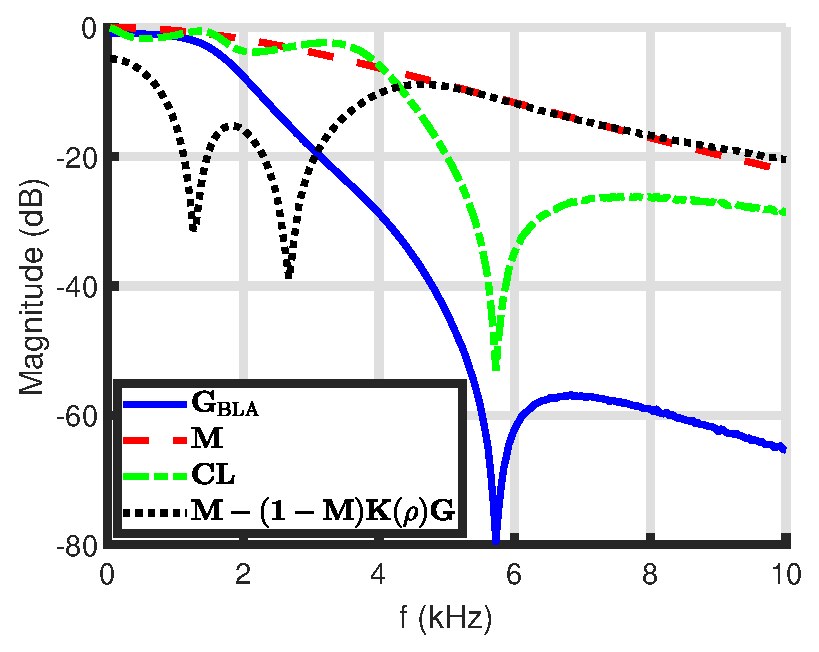
\includegraphics[width = 0.65\textwidth]{figures/real_system_nonparametric_closed_loop.eps}
\caption{Nonparametric estimates of the FRF of $G_{\mathrm{BLA}}(s)$, the reference model $M(s)$, the closed loop system $\mathrm{CL}(s)$ and the stability criteria $[M - (1-M)K(\rho_{\mathrm{opt}})G]$.}
\label{fig:GBLA_M_CL_nonparam}
\end{figure}

Additionally, the stability criteria $[M - (1-M)K(\rho_{\mathrm{opt}})G]$ are also plotted in figure \ref{fig:GBLA_M_CL_nonparam}. This quantity is below 1 in amplitude (0 dB) for all excited harmonics $\kexc$, which means that the stability of the closed might be guaranteed. To guarantee the stability of the closed loop system, the system $G_{\mathrm{BLA}}$ must be stable. This is the case. Moreover, $\frac{M(s)}{1-M(s)}$ must also be stable. The poles of $\frac{M(s)}{1-M(s)}$ are shown in figure \ref{fig:M_one_minus_M_poles}. None of the poles are in the right half plane, which means that $\frac{M(s)}{1-M(s)}$ is stable. Finally, we have only shown that $[M - (1-M)K(\rho_{\mathrm{opt}})G]$ is below 1 in amplitude for the excited frequencies. Therefore, we must also assume that the frequency resolution $f_s/N$ is high enough to ensure that no resonance peaks are missed. We must also assume that $[M - (1-M)K(\rho_{\mathrm{opt}})G]$ remains below 1 in amplitude for $f > 10 \, \mathrm{kHz}$. Assuming these things, the stability of the closed loop system is guaranteed.

\begin{figure}[H]
\centering
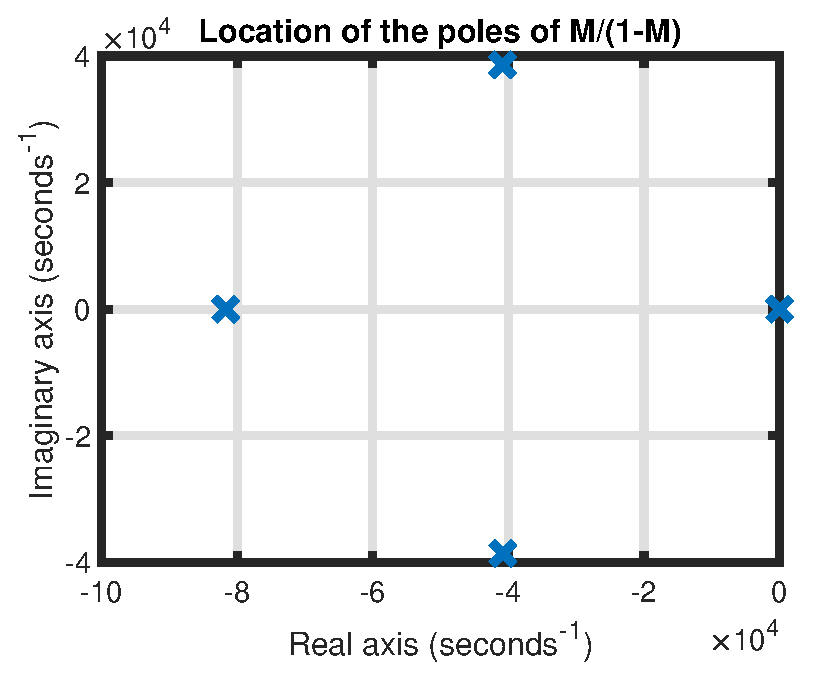
\includegraphics[width = 0.65\textwidth]{figures/M_one_minus_M_poles.eps}
\caption{Location of the poles of $\frac{M(s)}{1-M(s)}$}
\label{fig:M_one_minus_M_poles}
\end{figure}

\subsection{Controller realization}
The analog controller is built using TL074 operational amplifiers (OPAMP). The schematic is shown in figure \ref{fig:controller_schematic}. The capacitor in the integrator has a resistor
in parallel in order to limit the DC gain of the integrator. Extra components were also added to the second differentiator to limit the high-frequency (HF) gain as it was observed experimentally that the output of the second differentiator was very noisy without those components.

\begin{figure}[p]
	\centering
    
\includegraphics[angle=90,height=\textheight]{figures/circuit_annotated.jpg}
    \caption{Schematic of the controller.}
    \label{fig:controller_schematic}
\end{figure}

The controller was simulated in LTspice XVII.\footnote{\url{https://www.analog.com/en/design-center/design-tools-and-calculators/ltspice-simulator.html} (visited on 3 August 2020)} The FRF of the simulated analog controller is compared to the optimal controller $K(\rho_{\mathrm{opt}})$ in figure \ref{fig:controller_simulation}. The red dotted line shows the FRF of the simulated controller if no extra resitor and capacitor are added to the second differentiator. The gain almost reaches 120 dB. However, in this case, the HF gain still goes to zero due to the limitations of the TL074 OPAMPs. The blue dash-dotted line shows the simulated controller with the components added to the second differentiator. The maximal gain decreases significantly. Finally, the discrepancy in the low frequencies is due to the finite DC gain of the integrator. In the frequency range of interest, which is between 10 Hz and 10 kHz, the difference between the optimal controller and the simulated controller is not very significant.


\begin{figure}[H]
\centering
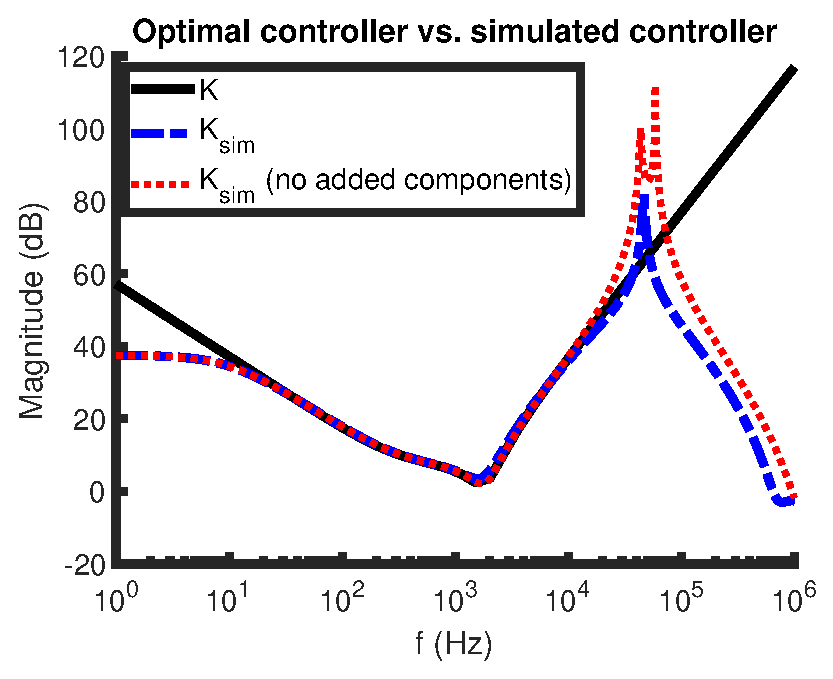
\includegraphics[width = 0.65\textwidth]{figures/controller_simulation.eps}
\caption{Optimal controller $K(\rho_\mathrm{opt})$ vs. the simulated controller from figure \ref{fig:controller_schematic}, with and without added resistor and capacitor to the second differentiator.}
\label{fig:controller_simulation}
\end{figure}


\newpage
The controller was soldered on a stripboard. The realized controller is shown in figure \ref{fig:controller_real}.

\begin{figure}
\centering
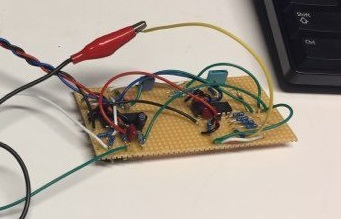
\includegraphics[width = 0.65\textwidth]{figures/controller_real.jpg}
\caption{Built controller.}
\label{fig:controller_real}
\end{figure}


The controller was measured with the measurement set-up (figure \ref{fig:set-up}). The excitation has the same properties as the excitation signal in section \ref{sec:nonparametric_estimate_controller}, except for one thing: the sine component amplitude is not flat. The amplitudes $A_k$ were shaped such that the energy is high at frequencies where the gain is expected to be low. The amplitudes are inversely proportional to the magnitude of the optimal controller $K(\rho_{\mathrm{opt}})$. The energy of the signal is also different. It is now $29.3 \, \mathrm{mV}_\mathrm{RMS}$. The amplitude spectrum of the input excitation used to measure the controller is shown in figure \ref{fig:controller_input_for_meas}.


\begin{figure}[H]
\centering
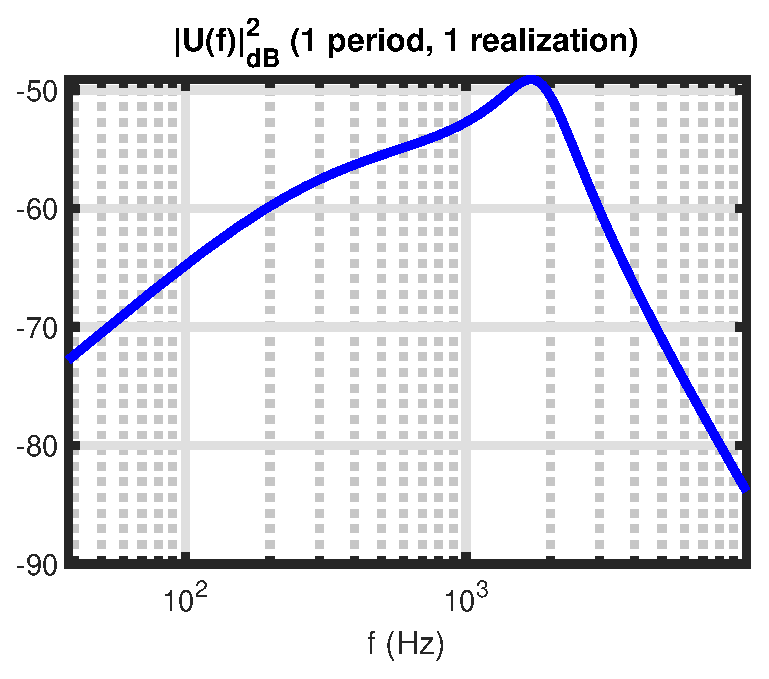
\includegraphics[width = 0.65\textwidth]{figures/controller_input_for_meas.eps}
\caption{Amplitude spectrum of one period of one realization of the input excitation used to measure the controller.}
\label{fig:controller_input_for_meas}
\end{figure}

\newpage
The nonparametric estimate of the FRF of the analog controller is shown in figure \ref{fig:controller_nonparam_measure}. The realized controller does not conform to the optimal controller $K(s,\rho_{\mathrm{opt}})$. However, as will be explained further, we believe these measurements to be invalid.

\begin{figure}[H]
\centering
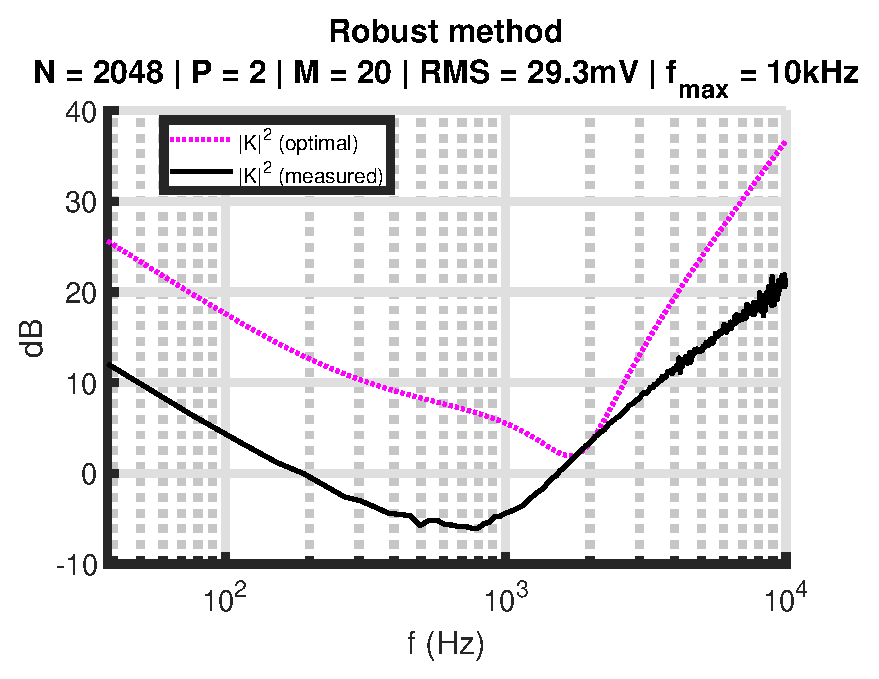
\includegraphics[width = 0.65\textwidth]{figures/robust_method_K.eps}
\caption{Nonparametric estimate of the FRF of the analog controller.}
\label{fig:controller_nonparam_measure}
\end{figure}

\newpage
\subsection{Closed loop}
Next, the Wiener-Hammerstein system was connected to the controller in closed loop with unity negative feedback (figure \ref{fig:closed_loop_system}). The same properties of the excitation signal that were used in sections \ref{sec:nonparametric_estimate_controller} and \ref{sec:controller_design_controller} are used here. One exception is the shape of the amplitude spectrum $A_k$. The best linear approximation of the Wiener-Hammerstein system depends on the energy of the input to that system as it is nonlinear. The reference signal was shaped in order to make sure that the input to the system is close to flat with an energy of $100 \, \mathrm{mV}_\mathrm{RMS}$. Now the amplitude spectrum of the reference signal is inversely proportional to the magnitude of the TF between the reference and the input to the system, which is $\frac{G(s)}{1+K(s,\rho_\mathrm{opt}) G(s)}$. This also changes the energy of the reference signal. It is now $42.9 \, \mathrm{mV}_\mathrm{RMS}$. The resulting nonparametric estimate of the FRF of the closed loop system is shown in figure \ref{fig:CL_measure}. The result is quite close to the optimal closed loop FRF (\ref{eq:optimal_CL}). Moreover, the closed loop system is stable.

\begin{figure}[H]
\centering
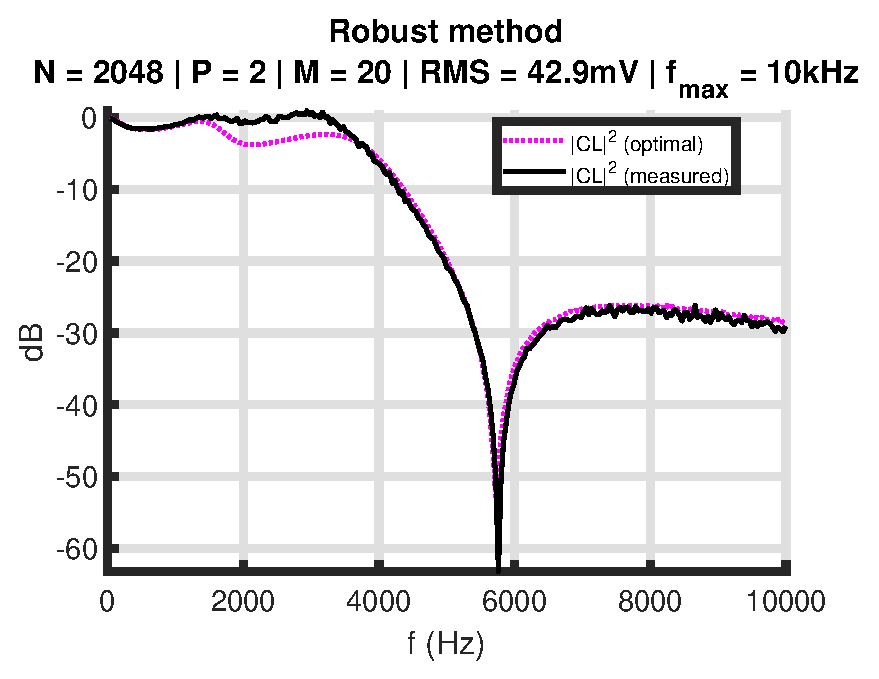
\includegraphics[width = 0.65\textwidth]{figures/robust_method_CL.eps}
\caption{Nonparametric estimate of the FRF of the closed loop system.}
\label{fig:CL_measure}
\end{figure}

\newpage
The success of the measurement of the closed loop system suggests that the nonparametric estimate of the FRF of the analog controller is invalid. We can estimate the FRF of the analog controller indirectly from the estimated closed loop FRF $\hat{\textrm{CL}}(j\omega_k)$ and the estimated FRF of the best linear approximation of the system $\hat G_{\mathrm{BLA}}(j\omega_k)$.
\begin{equation*}
	\hat{K}_{\mathrm{indirect}}(j\omega_k) =  \frac{\hat{\textrm{CL}}(j\omega_k)}{\hat G_{\mathrm{BLA}}(j\omega_k)(1-\hat{\textrm{CL}}(j\omega_k))}
\end{equation*}
The indirect estimate of the FRF of the controller is shown in figure \ref{fig:K_from_G_CL}. The controller is very close to the optimal controller. The indirect estimate spikes around $5.6 \, \mathrm{kHz}$, but this is just because the FRF of the system and the FRF of the closed loop system are zero around that frequency, which results in a division of zero by zero.

\begin{figure}[H]
\centering
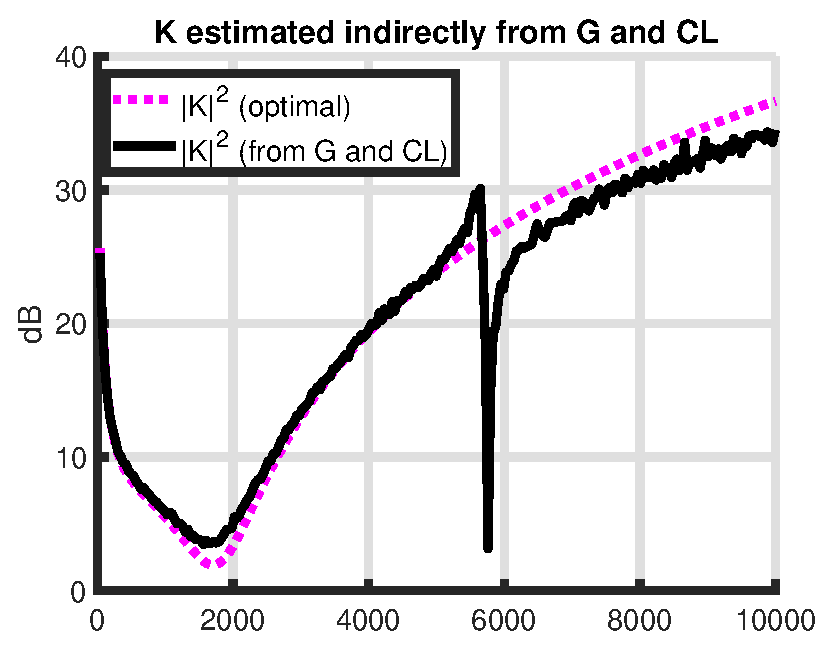
\includegraphics[width = 0.65\textwidth]{figures/K_from_G_CL.eps}
\caption{Indirect estimate of the FRF of the controller from $\hat{\textrm{CL}}(j\omega_k)$ and $G_{\mathrm{BLA}}(j\omega_k)$.}
\label{fig:K_from_G_CL}
\end{figure}

\section{Conclusion}
The FD method was used to design an analog controller for a Wiener-Hammerstein system. The stability constraints were used to guarantee the stability of the closed loop system. Then, the analog controller was constructed successfully. Finally, the analog controller and closed loop system were measured. However, the measurement of the analog controller was not successful. The cause of this failure is unknown.

\chapter*{Conclusion}
\addcontentsline{toc}{chapter}{Conclusion}
This work started with a summary of basic and advanced methods for estimating nonparametric models of LTI systems. Then, a review of data-driven model reference control was given. The cost functions were formulated in the time domain. However, by translating these formulations into the frequency domain it becomes clear that nonparametric models are hidden in the maths.

We then proposed to combine advanced methods for estimating nonparametric models with data-driven model reference control. A weighted nonlinear least squares cost function was also proposed. The time domain, frequency domain and weighted nonlinear least squares methods were applied to discrete-time systems. The weighted nonlinear least squares method greatly improves the quality of the controller in the case that the ideal controller is realizable. However, in most cases the original time domain method works better than the others.

The advantage of the proposed frequency domain method is that it is more general as it can also be applied to continuous-time systems. A nonparametric model of a continuous-time system was estimated and this was used to design an analog controller. Moreover, a review was given of constraints that guarantee the stability of the closed loop system. These constraints were used to verify that the designed controller would not destabilize the system.

\paragraph{Future work}
Model reference control is useful for finding a controller when input-output data of the uncontrolled system are available. This input-output data can be used to find a nonparametric model of the frequency response function of the system, which can then be used to find a suitable controller. However, it is still useful to have a parametric model of the system for the sake of interpretation.

An area where model reference control could be beneficial is in the control of time-varying systems. A linear parametric model can be estimated for the system, which can be used to design a controller. Afterwards, the controller can be adapted over time by using model reference control. This way, the interpretability of parametric models and the simplicity of nonparametric models can be combined into an adaptive control scheme. Employing nonparametric estimation of time-varying systems might also prove to be useful in this regard \cite{Lataire_time-varying}.


\paragraph{Contributions}
This work started when my supervisors pointed me to a paper comparing model-based and data-driven control \cite{comparison_model-based_data-driven}. In that paper, the correlation-based approach was mentioned. This led me to a paper on model reference control \cite{Data-driven_model_reference_control}. I was able to recreate the results presented in that paper. Afterwards, while trying to understand the correlation-based approach in depth, I noticed that nonparametric models of the frequency response function of the uncontrolled system were hiding in the mathematics. This then led to the use of more advanced nonparametric frequency domain methods. Finally, I realized that working in the frequency domain also allows for a generalization of the methods to continuous-time systems.


\chapter*{Software}
\addcontentsline{toc}{chapter}{Software}
The simulations in this thesis were coded in MATLAB \cite{MATLAB}. The Frequency Domain toolbox \cite{pintelon_book} supplied the necessary functions needed for estimating nonparametric models of the FRF with the robust LPM. The IniConfig class for \mbox{MATLAB} \cite{iniconfig} was very helpful in keeping everything organized. The Multi-Parametric Toolbox for MATLAB \cite{MPT3} was useful for doing convex optimization. Finally, LTspice XVII was used for simulating the analog controller before soldering it.

\bibliographystyle{vancouver}
\bibliography{references}
\addcontentsline{toc}{chapter}{Bibliography}



\end{document}          